%%% !TEX TS-program = XeLaTeX
%%%
%%%  پروژه کارشناسی — دانشگاه صنعتی امیرکبیر (پلی‌تکنیک تهران)
%%%  «طراحی و پیاده‌سازی یک مقیاس‌گذار خودکار سفارشی مبتنی بر معیارهای
%%%   Prometheus برای ریزخدمت‌های ابری»
%%%
%%%  بر پایه‌ی کلاس AUTthesis (نسخه‌ی آبان ۱۳۹۷).
%%%
%%%  روش اجرا:
%%%      xelatex AUTthesis
%%%      bibtex  AUTthesis
%%%      xelatex AUTthesis
%%%      xelatex AUTthesis
%%%  (برای ساخت نمایه، دستور xindy یا makeindex نیز لازم است — به README نگاه کنید.)
%%%
%%%  پیش‌نیاز قلم‌ها: B Nazanin، و در صورت فعال بودن، PGaramond و IranNastaliq.
%%%  فایل commands.tex برای نبودِ دو قلم دوم راه گریز دارد.

\documentclass[oneside,bsc,12pt]{AUTthesis}

% در این فایل، دستورها و تنظیمات مورد نیاز آورده شده است.
% بر پایه‌ی commands.tex الگوی رسمی AUTthesis، با افزوده‌های زیر:
%   • بسته‌های listings، tikz، longtable، booktabs و float برای قطعه‌کدها،
%     نمودارهای برداری و جدول‌های بلند.
%   • راه گریز برای قلم‌های PGaramond و IranNastaliq که روی هر سامانه‌ای نصب نیستند.
%-------------------------------------------------------------------------------

% در نسخه‌ی جدید زی‌پرشین، برای تایپ متن‌های ریاضی این سه بسته باید فراخوانی شود.
\usepackage{amsthm,amssymb,amsmath,amsfonts}

% حاشیه‌های صفحه، مطابق دستورالعمل تحصیلات تکمیلی دانشگاه
\usepackage[top=30mm, bottom=30mm, left=25mm, right=30mm]{geometry}

\usepackage{graphicx}
\usepackage{color}
\usepackage{xcolor}
\usepackage{setspace}
\usepackage{titletoc}
\usepackage{tocloft}
\usepackage{enumitem}

% جدول‌ها
\usepackage{array}
\usepackage{longtable}
\usepackage{multirow}
\usepackage{booktabs}

% شکل‌ها
\usepackage{float}

% قطعه‌کدها
\usepackage{listings}

% نمودارهای برداری
\usepackage{tikz}
\usetikzlibrary{positioning,arrows.meta,shapes.geometric,fit,calc,backgrounds}

% لینک‌های رنگی. برای نسخه‌ی نهایی چاپی، خط زیر را غیرفعال و خط پس از آن را فعال کنید.
\usepackage[pagebackref=false,colorlinks,linkcolor=blue,citecolor=red]{hyperref}
%\usepackage[pagebackref=false]{hyperref}

\usepackage[nameinlink]{cleveref}
\AtBeginDocument{%
    \crefname{equation}{برابری}{equations}%
    \crefname{chapter}{فصل}{chapters}%
    \crefname{section}{بخش}{sections}%
    \crefname{appendix}{پیوست}{appendices}%
    \crefname{enumi}{مورد}{items}%
    \crefname{footnote}{زیرنویس}{footnotes}%
    \crefname{figure}{شکل}{figures}%
    \crefname{table}{جدول}{tables}%
    \crefname{theorem}{قضیه}{theorems}%
    \crefname{lemma}{لم}{lemmas}%
    \crefname{corollary}{نتیجه}{corollaries}%
    \crefname{proposition}{گزاره}{propositions}%
    \crefname{definition}{تعریف}{definitions}%
    \crefname{result}{نتیجه}{results}%
    \crefname{example}{مثال}{examples}%
    \crefname{remark}{نکته}{remarks}%
    \crefname{note}{یادداشت}{notes}%
}

\usepackage{fancyhdr}
\usepackage[nottoc]{tocbibind}
\usepackage{makeidx,multicol}
\setlength{\columnsep}{1.5cm}

\usepackage{verbatim}
\makeindex
\usepackage{sectsty}

% فراخوانی زی‌پرشین و تعریف قلم‌ها
\usepackage{xepersian}
\SepMark{-}
\settextfont[Scale=1.2]{B Nazanin}
\setlatintextfont{Times New Roman}
\renewcommand{\labelitemi}{$\bullet$}

%-------------------------------------------------------------------------------
% ارقام فرمول‌ها
%
% الگوی رسمی این خط را فعال دارد تا ارقامِ داخل فرمول‌ها فارسی شود، و برای این کار
% قلم PGaramond لازم است. اگر آن قلم روی سامانه‌ی شما نصب است، خط زیر را فعال کنید.
% در حالت غیرفعال، ارقامِ فرمول‌ها لاتین می‌مانند — که برای متنی با این حجم از
% عبارت‌های عددی و نام‌های لاتین، خواناتر هم هست.
%\setdigitfont[Scale=1.1]{PGaramond}
%-------------------------------------------------------------------------------

% قلم نستعلیق. الگوی رسمی از آن تنها در صفحه‌های «تقدیم» و «سپاس‌گزاری» استفاده
% می‌کند و هر دو صفحه در این نوشتار حذف شده‌اند، پس این تعریف در حال حاضر
% بی‌استفاده است؛ نگه داشته شده تا اگر بعداً یکی از آن صفحه‌ها بازگردد آماده باشد.
\defpersianfont\nastaliq[Scale=2]{IranNastaliq}

\defpersianfont\chapternumber[Scale=3]{B Nazanin}

\renewcommand\proofname{\textbf{برهان}}
\renewcommand{\bibname}{منابع و مراجع}

%-------------------------------------------------------------------------------
% تنظیم قطعه‌کدها
%
% هر قطعه‌کد باید داخل محیط latin قرار گیرد تا جهت آن چپ‌به‌راست بماند. برای
% کوتاه‌شدن کار، محیط‌های آماده‌ی زیر تعریف شده‌اند.
%-------------------------------------------------------------------------------
\definecolor{codebg}{rgb}{0.97,0.97,0.97}
\definecolor{codecomment}{rgb}{0.35,0.45,0.35}
\definecolor{codekeyword}{rgb}{0.20,0.20,0.60}
\definecolor{codestring}{rgb}{0.55,0.25,0.25}

\lstset{
  basicstyle=\ttfamily\footnotesize,
  backgroundcolor=\color{codebg},
  commentstyle=\color{codecomment}\itshape,
  keywordstyle=\color{codekeyword}\bfseries,
  stringstyle=\color{codestring},
  frame=single,
  rulecolor=\color{black!30},
  breaklines=true,
  breakatwhitespace=true,
  columns=fullflexible,
  keepspaces=true,
  showstringspaces=false,
  tabsize=2,
  captionpos=b,
  xleftmargin=1em,
  xrightmargin=1em,
  aboveskip=1em,
  belowskip=1em,
}

% زبان‌های به‌کاررفته در این نوشتار
\lstdefinelanguage{promql}{
  keywords={sum,rate,count,increase,avg,max,min,by,without,offset},
  sensitive=true,
  comment=[l]{\#},
  morestring=[b]",
}
\lstdefinelanguage{yamlx}{
  keywords={true,false,null},
  sensitive=false,
  comment=[l]{\#},
  morestring=[b]",
}

% محیط آماده: قطعه‌کد چپ‌به‌راست
\lstnewenvironment{latincode}[1][]
  {\setLTR\lstset{#1}}
  {}

%-------------------------------------------------------------------------------
% ماکروهای کمکی این نوشتار
%-------------------------------------------------------------------------------
% یک شناسه‌ی لاتین در میان متن فارسی (نام بسته، نام تابع، نام بازو، …)
\DeclareRobustCommand{\code}[1]{\lr{\texttt{\small #1}}}
% یک عدد یا واحد لاتین در میان متن فارسی
\DeclareRobustCommand{\num}[1]{\lr{#1}}
% نام یک بازوی مقایسه
\DeclareRobustCommand{\arm}[1]{\lr{\texttt{\small #1}}}
% ارجاع به دفترچه‌ی آزمایشگاه (فقط در نسخه‌های پیش‌نویس؛ در متن نهایی استفاده نشده)
\DeclareRobustCommand{\notebookref}[1]{\textsuperscript{[د.آ. #1]}}

%-------------------------------------------------------------------------------
% سرصفحه‌های فهرست‌ها
%-------------------------------------------------------------------------------
\setlength{\cftbeforetoctitleskip}{-1.2em}
\setlength{\cftbeforelottitleskip}{-1.2em}
\setlength{\cftbeforeloftitleskip}{-1.2em}
\setlength{\cftaftertoctitleskip}{-1em}
\setlength{\cftafterlottitleskip}{-1em}
\setlength{\cftafterloftitleskip}{-1em}

\newcommand\tocheading{\par عنوان\hfill صفحه \par}
\newcommand\lofheading{\hspace*{.5cm}\figurename\hfill صفحه \par}
\newcommand\lotheading{\hspace*{.5cm}\tablename\hfill صفحه \par}

\renewcommand{\cftchapleader}{\cftdotfill{\cftdotsep}}
\renewcommand{\cfttoctitlefont}{\hspace*{\fill}\LARGE\bfseries}
\renewcommand{\cftaftertoctitle}{\hspace*{\fill}}
\renewcommand{\cftlottitlefont}{\hspace*{\fill}\LARGE\bfseries}
\renewcommand{\cftafterlottitle}{\hspace*{\fill}}
\renewcommand{\cftloftitlefont}{\hspace*{\fill}\LARGE\bfseries}
\renewcommand{\cftafterloftitle}{\hspace*{\fill}}

%-------------------------------------------------------------------------------
% قضیه‌ها، تعریف‌ها و نمونه‌ها
%-------------------------------------------------------------------------------
\theoremstyle{definition}
\newtheorem{definition}{تعریف}[section]
\newtheorem{remark}[definition]{نکته}
\newtheorem{note}[definition]{یادداشت}
\newtheorem{example}[definition]{نمونه}
\newtheorem{question}[definition]{سوال}
\newtheorem{remember}[definition]{یاداوری}
\theoremstyle{theorem}
\newtheorem{theorem}[definition]{قضیه}
\newtheorem{lemma}[definition]{لم}
\newtheorem{proposition}[definition]{گزاره}
\newtheorem{corollary}[definition]{نتیجه}

%-------------------------------------------------------------------------------
% صفحه‌های آغاز فصل
%-------------------------------------------------------------------------------
\makeatletter
\newcommand\mycustomraggedright{%
 \if@RTL\raggedleft%
 \else\raggedright%
 \fi}
\def\@makechapterhead#1{%
\thispagestyle{style1}
\vspace*{20\p@}%
{\parindent \z@ \mycustomraggedright
\ifnum \c@secnumdepth >\m@ne
\if@mainmatter

\bfseries{\Huge \@chapapp}\small\space {\chapternumber\thechapter}
\par\nobreak
\vskip 0\p@
\fi
\fi
\interlinepenalty\@M
\Huge \bfseries #1\par\nobreak
\vskip 120\p@

}
\newpage}
\bidi@patchcmd{\@makechapterhead}{\thechapter}{\tartibi{chapter}}{}{}
\bidi@patchcmd{\chaptermark}{\thechapter}{\tartibi{chapter}}{}{}
\makeatother

\pagestyle{fancy}
\renewcommand{\chaptermark}[1]{\markboth{\chaptername~\tartibi{chapter}: #1}{}}

\fancypagestyle{style1}{
\fancyhf{}
\fancyfoot[c]{\thepage}
\fancyhead[R]{\leftmark}%
\renewcommand{\headrulewidth}{1.2pt}
}

\fancypagestyle{style2}{
\fancyhf{}
\fancyhead[R]{چکیده}
\fancyfoot[C]{\thepage{}}
\renewcommand{\headrulewidth}{1.2pt}
}

\fancypagestyle{style3}{%
  \fancyhf{}%
  \fancyhead[R]{فهرست نمادها}
  \fancyfoot[C]{\thepage}%
  \renewcommand{\headrulewidth}{1.2pt}%
}

\fancypagestyle{style4}{%
  \fancyhf{}%
  \fancyhead[R]{فهرست جداول}
  \fancyfoot[C]{\thepage}%
  \renewcommand{\headrulewidth}{1.2pt}%
}

\fancypagestyle{style5}{%
  \fancyhf{}%
  \fancyhead[R]{فهرست اشکال}
  \fancyfoot[C]{\thepage}%
  \renewcommand{\headrulewidth}{1.2pt}%
}

\fancypagestyle{style6}{%
  \fancyhf{}%
  \fancyhead[R]{فهرست مطالب}
  \fancyfoot[C]{\thepage}%
  \renewcommand{\headrulewidth}{1.2pt}%
}

\fancypagestyle{style7}{%
  \fancyhf{}%
  \fancyhead[R]{نمایه}
  \fancyfoot[C]{\thepage}%
  \renewcommand{\headrulewidth}{1.2pt}%
}

\fancypagestyle{style8}{%
  \fancyhf{}%
  \fancyhead[R]{منابع و مراجع}
  \fancyfoot[C]{\thepage}%
  \renewcommand{\headrulewidth}{1.2pt}%
}
\fancypagestyle{style9}{%
  \fancyhf{}%
  \fancyhead[R]{واژه‌نامه‌ی فارسی به انگلیسی}
  \fancyfoot[C]{\thepage}%
  \renewcommand{\headrulewidth}{1.2pt}%
}

% حذف نام فهرست تصاویر و فهرست جداول از فهرست مطالب
\newcommand*{\BeginNoToc}{%
  \addtocontents{toc}{%
    \edef\protect\SavedTocDepth{\protect\the\protect\value{tocdepth}}%
  }%
  \addtocontents{toc}{%
    \protect\setcounter{tocdepth}{-10}%
  }%
}
\newcommand*{\EndNoToc}{%
  \addtocontents{toc}{%
    \protect\setcounter{tocdepth}{\protect\SavedTocDepth}%
  }%
}
\newcounter{savepage}
\renewcommand{\listfigurename}{فهرست اشکال}
\renewcommand{\listtablename}{فهرست جداول}


\begin{document}
\baselineskip=.75cm
\linespread{1.75}

% صفحه‌ی عنوان، چکیده‌ی فارسی و کلیدواژه‌ها
%% -!TEX root = AUTthesis.tex
% مشخصات پروژه، عنوان، و چکیده‌ی فارسی.
% جدول مشخصات و صفحه‌ی عنوان به‌طور خودکار از روی این مقادیر ساخته می‌شود.
%%%%%%%%%%%%%%%%%%%%%%%%%%%%%%%%%%%%

\faculty{دانشکده مهندسی کامپیوتر}

% بدون گرایش
\department{}

\fatitle{طراحی و پیاده‌سازی یک مقیاس‌گذار خودکار سفارشی
\\[.4cm]
مبتنی بر معیارهای \lr{Prometheus} برای ریزخدمت‌های ابری}

\firstsupervisor{دکتر سید احمد جوادی}
%\secondsupervisor{استاد راهنمای دوم}

% استاد مشاور ندارد؛ خط زیر عمداً غیرفعال است.
%\firstadvisor{نام کامل استاد مشاور}
%\secondadvisor{استاد مشاور دوم}

\internalexaminer{دکتر حامد فربه}
%\externalexaminer{استاد داور دوم}

\name{رائین }
\surname{سلطانی}

%%%%%%%%%%%%%%%%%%%%%%%%%%%%%%%%%%
\thesisdate{شهریور ۱۴۰۵}

% چکیده‌ی فارسی
\fa-abstract{
مقیاس‌گذار افقی پیش‌فرض \lr{Kubernetes}، یعنی \lr{Horizontal Pod Autoscaler}، عمدتاً بر مصرف
پردازنده تکیه می‌کند و کاملاً واکنشی است؛ راه حل متعارف برای دومی، افزودن پیش‌بینی است.
در این پروژه یک مقیاس‌گذار سفارشی به زبان \lr{Go} پیاده‌سازی شد که سیگنال را با عبارت
\lr{PromQL} از \lr{Prometheus} می‌خواند و سه سیاست دارد: آستانه‌ای، پیش‌بینانه بر پایه‌ی بار
کل، و پیش‌بینانه بر پایه‌ی بار هر نمونه.

یافته‌ی اصلی اما به پایداری حلقه‌ی بسته مربوط است و نه به خودِ مقیاس‌گذار. پیش‌بینی بار هر
نمونه، سیگنالی را برون‌یابی می‌کند که کنش‌های خود کنترل‌گر آن را جابه‌جا می‌کند، و حلقه بهره‌ی
مثبت پیدا می‌کند. این ناپایداری در سنجه‌های متعارف کیفیت
خدمت و هزینه تقریباً نامرئی است، چون سازوکار پایدارسازی آن را می‌پوشاند. با برداشتن این
سازوکار، همان سیاست در یک اجرای ۱۸۰۰ ثانیه‌ای با ۱۲۰ چرخه‌ی کنترل، ۱۱۹ بار تغییر جهت می‌دهد و
نقض کیفیت خدمت آن به ۵۰/۸ درصد می‌رسد، حال آنکه با پنجره‌ی پایدارسازی ۹۰ ثانیه‌ای از همه‌ی
آزمون‌ها سربلند بیرون می‌آید. دو تکرار مستقل همین امضا را بازتولید کردند (۱۱۹ و ۱۱۵ تغییر جهت).

ارزیابی روی یک خوشه‌ی واقعی با چهار الگوی بار، نُه بازوی مقایسه و ۵۳ اجرای معتبر انجام شد.
در میان بازوهای خودکار، سیاست پیش‌بینانه‌ی درست روی هر چهار الگو کم‌ترین کم‌تأمین منابع و
کم‌ترین یا هم‌تراز کم‌ترین نقض کیفیت خدمت را دارد، و روی الگوی روزانه نزدیک به چهار برابر
سریع‌تر از مقیاس‌گذار پیش‌فرض با همان سنجه‌ی سفارشی واکنش نشان می‌دهد؛ بهای آن ۵/۷ تا ۲۰/۲ درصد
ظرفیت بیشتر است. تأمین ایستا در سطح اوج کیفیت خدمت بهتری می‌دهد، با ظرفیتی به‌مراتب بیشتر.
پس ادعای قابل دفاع یک مبادله است و نه برتری مطلق. از نظر روش‌شناختی، ارزیابی پایداری
باید میراگر را خاموش کند و بار پله‌ای بدهد، وگرنه چیزی را می‌سنجد که پیشاپیش پنهان شده است.
}

% کلیدواژه‌ها
\keywords{مقیاس‌گذاری خودکار، \lr{Kubernetes}، \lr{Prometheus}، مقیاس‌گذاری پیش‌بینانه، پایداری حلقه‌ی بسته، ریزخدمت}

\AUTtitle
%%%%%%%%%%%%%%%%%%%%%%%%%%%%%%%%%%
\vspace*{7cm}
\thispagestyle{empty}
\begin{center}

\includegraphics[height=5cm,width=12cm]{besm}
\end{center}


% تاییدیه‌ی هیئت داوران
\newpage
\thispagestyle{empty}

\section*{صفحه فرم ارزیابی و تصویب پروژه — فرم تأیید اعضای کمیته دفاع}

\fontsize{12pt}{14pt}\selectfont
\vspace*{1cm}

در این صفحه، فرم دفاع (فرم کمیته دفاع، موجود در پرونده آموزشی) قرار می‌گیرد.

\vspace*{1cm}

\subsection*{نکات مهم:}

\begin{itemize}
\item
	نگارش پروژه/پایان‌نامه باید به
	{\color{red} زبان فارسی}
	و بر اساس آخرین نسخه دستورالعمل و راهنمای تدوین پایان‌نامه‌های دانشگاه صنعتی امیرکبیر باشد.
\item رنگ جلد پروژه/پایان‌نامه چاپی کارشناسی، کارشناسی ارشد و دکترا باید به ترتیب مشکی، طوسی و سفید رنگ باشد.
\item چاپ و صحافی پروژه/پایان‌نامه به‌صورت
{\color{red} پشت و رو (دورو)}
بلامانع است و انجام آن توصیه می‌شود.
\end{itemize}

%%%%%%%%%%%%%%%%%%%%%%%%%%%%%%%%%%%%%%%%%%%%%%%%%%%%%%%%%%%%%%%%%%%%%%%%%%%%%%%%%
\newpage
\thispagestyle{empty}
\begin{picture}(50,50)
  \put(17,0){
\includegraphics[scale=1.1]{fa-logo}}
  \put(4.5,-13){\footnotesize{دانشگاه صنعتی امیرکبیر}}
  \put(10.5,-27){\footnotesize{(پلی‌تکنیک تهران)}}
  \put(170,30){\bf{به نام خدا}}
  \put(140,-5){\Large\bf{تعهدنامه اصالت اثر}}
  \put(310,0){تاریخ: \datethesis}
\end{picture}

\vspace*{2.5cm}

اینجانب {\bf{\fname\lname}} متعهد می‌شوم که مطالب مندرج در این پروژه حاصل کار پژوهشی اینجانب تحت نظارت و راهنمایی اساتید دانشگاه صنعتی امیرکبیر بوده و به دستاوردهای دیگران که در این پژوهش از آن‌ها استفاده شده است مطابق مقررات و روال متعارف ارجاع و در فهرست منابع و مآخذ ذکر گردیده است. این پروژه قبلاً برای احراز هیچ مدرک هم‌سطح یا بالاتر ارائه نگردیده است.

در صورت اثبات تخلف در هر زمان، مدرک تحصیلی صادر شده توسط دانشگاه از درجه اعتبار ساقط بوده و دانشگاه حق پیگیری قانونی خواهد داشت.

کلیه نتایج و حقوق حاصل از این پروژه متعلق به دانشگاه صنعتی امیرکبیر می‌باشد. هرگونه استفاده از نتایج علمی و عملی، واگذاری اطلاعات به دیگران یا چاپ و تکثیر، نسخه‌برداری، ترجمه و اقتباس از این پروژه بدون موافقت کتبی دانشگاه صنعتی امیرکبیر ممنوع است.
نقل مطالب با ذکر مآخذ بلامانع است.\\
\vspace{2.5cm}

{\centerline {\bf{\fname\lname}}}
\vspace*{.2cm}
{\centerline{امضا}}
%%%%%%%%%%%%%%%%%%%%%%%%%%%%%%%%%


% صفحه‌های «تقدیم» و «سپاس‌گزاری» حذف شده‌اند.
% فایل زیر تنها صفحه‌ی چکیده‌ی فارسی را تولید می‌کند.
%%%%%%%%%%%%%%%%%%%%%%%%%%%%%%%%%%%%
% ------------------------------------------------------------------------------
% سپاس‌گزاری.
%
% این صفحه نیز شخصی است. متن زیر یک پیش‌نویس است؛ پیش از تحویل نهایی بازنویسی‌اش
% کنید.
% ------------------------------------------------------------------------------
\newpage\thispagestyle{empty}
{\nastaliq
سپاس‌گزاری
}
\\[2cm]

از استاد راهنمای این پروژه، جناب آقای دکتر سید احمد جوادی، سپاس‌گزارم. راهنمایی ایشان در
شکل‌گیری پرسش این پروژه نقش تعیین‌کننده داشت: آنچه در آغاز «ساختن یک مقیاس‌گذار خودکار» بود،
در گفت‌وگو با ایشان به پرسشی دقیق‌تر و قابل دفاع‌تر درباره‌ی پایداری حلقه‌ی کنترل تبدیل شد.

همچنین از دانشکده‌ی مهندسی کامپیوتر دانشگاه صنعتی امیرکبیر و از همه‌ی استادانی که در طول
دوره‌ی کارشناسی از آن‌ها آموختم، سپاس‌گزارم.

از خانواده‌ام که در تمام این سال‌ها پشتیبان من بودند، صمیمانه تشکر می‌کنم.

% با استفاده از دستور زیر، امضای شما به‌طور خودکار درج می‌شود.
\signature

%%%%%%%%%%%%%%%%%%%%%%%%%%%%%%%%%%%%%%%%%
%%%%%%%%%%%%%%%%%%%%%%%%%%%% کدهای زیر را تغییر ندهید.
\newpage\clearpage

\pagestyle{style2}

\vspace*{-1cm}
\section*{\centering چکیده}
\vspace*{.5cm}
\ffa-abstract
\vspace*{2cm}

{\noindent\large\textbf{واژه‌های کلیدی:}}\par
\vspace*{.5cm}
\fkeywords


% شماره‌گذاری صفحات پیش از فصل اول، با حروف ابجد
\pagenumbering{alph}

%-----------------------------------------------------------------------------
% فهرست مطالب، فهرست اشکال و فهرست جداول
\cleardoublepage
\pagestyle{style6}
\tableofcontents
\pagestyle{style6}
\cleardoublepage
%============
\BeginNoToc
\addtocontents{lof}{\lofheading}% سرصفحه‌ی نخستین صفحه‌ی فهرست اشکال
\pagestyle{style5}
\listoffigures
\thispagestyle{style5}
\cleardoublepage
%============
\addtocontents{lot}{\lotheading}% سرصفحه‌ی نخستین صفحه‌ی فهرست جداول
\thispagestyle{style4}
\listoftables
\thispagestyle{style4}
%============
\cleardoublepage
\setcounter{savepage}{\arabic{page}}
\mainmatter
\addtocontents{toc}{\tocheading}% سرصفحه‌ی نخستین صفحه‌ی فهرست مطالب
\EndNoToc


% فهرست نمادها و اختصارها
%%%%%%%%%%%%%

{\centering\LARGE\textbf{فهرست نمادها و اختصارها}\par}%

\pagenumbering{alph}
\setcounter{page}{\thesavepage}
\vspace*{1cm}

\pagestyle{style3}

\symb{\text{نماد}}{مفهوم}
\\
%%%%%%%%%%%%%%%%%%%%%%%%%%%%%%%%%%%%%%%%%%%%%%%%%%%%%%%%%
% نمادهای ریاضی به‌کاررفته در فصل‌های سوم تا پنجم
%%%%%%%%%%%%%%%%%%%%%%%%%%%%%%%%%%%%%%%%%%%%%%%%%%%%%%%%%
\symb{\lambda(t)}{
نرخ کل ورود درخواست‌ها در لحظه‌ی $t$، بر حسب درخواست بر ثانیه
}
\symb{m(t)}{
سنجه‌ی مشاهده‌شده به ازای هر نمونه‌ی آماده، یعنی $\lambda(t)/r(t)$
}
\symb{r(t)}{
تعداد نمونه‌های آماده در لحظه‌ی $t$، برابر با \lr{status.readyReplicas}
}
\symb{s(t)}{
تعداد نمونه‌های درخواست‌شده، برابر با \lr{spec.replicas}
}
\symb{T}{
نرخ هدف به ازای هر نمونه؛ در همه‌ی آزمایش‌ها برابر ۱۰۰ درخواست بر ثانیه
}
\symb{\varepsilon}{
پهنای نسبی ناحیه‌ی مرده؛ در همه‌ی آزمایش‌ها برابر ۰٫۱
}
\symb{\Delta t}{
فاصله‌ی زمانی آشتی‌دهی؛ در همه‌ی آزمایش‌ها برابر ۱۵ ثانیه
}
\symb{h}{
افق پیش‌بینی، بر حسب تعداد گام آشتی‌دهی؛ مقدار پیش‌فرض ۳
}
\symb{\alpha}{
ضریب هموارسازی نمایی سطح؛ مقدار پیش‌فرض ۰٫۵
}
\symb{\beta}{
ضریب هموارسازی روند در روش \lr{Holt}
}
\symb{\ell_k}{
مقدار هموارشده‌ی سطح در گام $k$
}
\symb{b_k}{
مقدار هموارشده‌ی روند (شیب) در گام $k$
}
\symb{\hat{\lambda}_{k+h}}{
پیش‌بینی بار کل برای $h$ گام پس از گام $k$
}
\symb{d_k}{
پیشنهاد خام سیاست در گام $k$، پیش از پایدارسازی
}
\symb{W}{
طول پنجره‌ی پایدارسازی مقیاس به پایین، بر حسب ثانیه؛ مقدار پیش‌فرض ۹۰
}
\symb{r_{\min},\,r_{\max}}{
کف و سقف مجاز تعداد نمونه؛ در همه‌ی آزمایش‌ها ۱ و ۲۰
}
\symb{R}{
هزینه بر حسب نمونه‑ثانیه، یعنی $\int r(t)\,dt$ روی پنجره‌ی اندازه‌گیری
}
\symb{U}{
کم‌تأمین منابع بر حسب نمونه‑ثانیه
}
\symb{O}{
بیش‌تأمین منابع بر حسب نمونه‑ثانیه
}
\symb{V}{
درصد زمان اجرا با نقض توافق سطح خدمت
}
\symb{N_{\mathrm{rev}}}{
تعداد تغییر جهت تصمیم‌های مقیاس‌گذاری
}

\vspace*{1cm}
{\centering\large\textbf{اختصارها}\par}
\vspace*{.5cm}

\symb{\text{HPA}}{
\lr{Horizontal Pod Autoscaler} — مقیاس‌گذار خودکار افقی پیش‌فرض \lr{Kubernetes}
}
\symb{\text{VPA}}{
\lr{Vertical Pod Autoscaler} — مقیاس‌گذار خودکار عمودی
}
\symb{\text{CA}}{
\lr{Cluster Autoscaler} — مقیاس‌گذار خودکار گره‌های خوشه
}
\symb{\text{KEDA}}{
\lr{Kubernetes Event-driven Autoscaling}
}
\symb{\text{SLA}}{
\lr{Service Level Agreement} — توافق سطح خدمت
}
\symb{\text{SLO}}{
\lr{Service Level Objective} — هدف سطح خدمت
}
\symb{\text{QoS}}{
\lr{Quality of Service} — کیفیت خدمت
}
\symb{\text{EWMA}}{
\lr{Exponentially Weighted Moving Average} — میانگین متحرک با وزن نمایی
}
\symb{\text{ARIMA}}{
\lr{AutoRegressive Integrated Moving Average}
}
\symb{\text{LSTM}}{
\lr{Long Short-Term Memory}
}
\symb{\text{CFS}}{
\lr{Completely Fair Scheduler} — زمان‌بند پردازنده‌ی لینوکس
}
\symb{\text{API}}{
\lr{Application Programming Interface} — واسط برنامه‌نویسی کاربردی
}
\symb{\text{CNCF}}{
\lr{Cloud Native Computing Foundation}
}

%%%%%%%%%%%%%%%%%%%%%%%%%%%%%%%%%%%%%%%

\thispagestyle{style3}
\newpage
%%%%%%%%%%%%%%%%%%%%%%%%%%%%%%%%%%%%%


\pagenumbering{arabic}
\pagestyle{style1}

%--------------------------------------------------------------------- فصل‌ها
\chapter{مقدمه}
\label{ch:intro}

\section{زمینه}
\label{sec:intro-background}

نرم‌افزارهای امروزی به‌شکل فزاینده‌ای روی زیرساخت‌های رایانش ابری\LTRfootnote{Cloud Computing}
مستقر می‌شوند و با معماری ریزخدمت\LTRfootnote{Microservice} توسعه می‌یابند. در این معماری،
یک سامانه‌ی بزرگ به مجموعه‌ای از سرویس‌های کوچک و مستقل شکسته می‌شود که هر یک جداگانه مستقر و
جداگانه مقیاس‌گذاری می‌شود. همین استقلال، امکانی را فراهم می‌کند که در معماری یکپارچه وجود
نداشت: ظرفیت را می‌توان دقیقاً به همان بخشی افزود که زیر فشار است، نه به کل سامانه.

مهم‌ترین مزیتی که رایانش ابری به این معماری اضافه می‌کند، کشسانی\LTRfootnote{Elasticity}
است؛ یعنی توانایی سامانه در افزودن یا کاستن خودکار منابع پردازشی متناسب با بار ورودی. هربست و
همکاران~\cite{herbst2013} در تعریف دقیقی که برای این مفهوم پیشنهاد کرده‌اند، کشسانی را از
مقیاس‌پذیری\LTRfootnote{Scalability} و کارایی\LTRfootnote{Efficiency} تفکیک می‌کنند:
مقیاس‌پذیری یک ویژگی ایستا است و می‌گوید سامانه \emph{می‌تواند} با منابع بیشتر بار بیشتری را
سرویس دهد، اما کشسانی یک ویژگی پویاست و می‌پرسد سامانه \emph{چقدر سریع و چقدر دقیق} خود را با
تغییر بار تطبیق می‌دهد. این تمایز برای کل این نوشتار پایه‌ای است، چون آنچه در فصل‌های بعد
اندازه‌گیری می‌شود سرعت و دقت تطبیق است و نه صرفاً امکان آن.

مدیریت درست منابع در این بستر، مسئله‌ای صرفاً فنی نیست. کم‌تأمین منابع مستقیماً به افت کیفیت
خدمت\LTRfootnote{Quality of Service (QoS)} و نقض توافق سطح خدمت\LTRfootnote{Service Level
Agreement (\lr{SLA})} تبدیل می‌شود، و بیش‌تأمین منابع مستقیماً هزینه‌ی زیرساخت است. ورما و
همکاران~\cite{verma2015} در گزارش سامانه‌ی \lr{Borg} در گوگل نشان می‌دهند که در مقیاس بزرگ،
اختلاف میان منابع درخواست‌شده و منابع واقعاً مصرف‌شده به هدر رفتن حجم عظیمی از ظرفیت می‌انجامد؛
و رزادسا و همکاران~\cite{rzadca2020} در معرفی \lr{Autopilot} همین مسئله را انگیزه‌ی اصلی
خودکارسازی تعیین منابع می‌دانند. به همین دلیل، مقیاس‌گذاری خودکار\LTRfootnote{Autoscaling} به
یکی از موضوعات اصلی نگهداشت سامانه‌های ابری تبدیل شده است.

\section{مقیاس‌گذاری خودکار و انواع آن}
\label{sec:intro-autoscaling}

مقیاس‌گذاری خودکار سه شکل رایج دارد. در \emph{مقیاس‌گذاری افقی}\LTRfootnote{Horizontal Scaling}
تعداد نمونه‌های سرویس تغییر می‌کند. در \emph{مقیاس‌گذاری عمودی}\LTRfootnote{Vertical Scaling}
منابع اختصاص‌یافته به هر نمونه (پردازنده و حافظه) تغییر می‌کند. در \emph{مقیاس‌گذاری خوشه}
تعداد گره‌های زیرساخت تغییر می‌کند. این پروژه تنها به شکل نخست می‌پردازد، که رایج‌ترین شکل در
سکوهای ارکستراسیون کانتینر است و در \lr{Kubernetes} با ابزار
\lr{Horizontal Pod Autoscaler (HPA)} پیاده‌سازی شده است.

از منظر سازوکار تصمیم‌گیری، دسته‌بندی مهم‌تری وجود دارد که کل این نوشتار بر پایه‌ی آن ساخته
شده است. لوریدو-بوتران و همکاران~\cite{lorido2014} در مرور جامع خود، روش‌های مقیاس‌گذاری
خودکار را به پنج خانواده تقسیم می‌کنند: قواعد آستانه‌ای ایستا، نظریه‌ی کنترل، یادگیری تقویتی،
نظریه‌ی صف، و تحلیل سری‌های زمانی. کیو و همکاران~\cite{qu2018} نیز در مرور دیگری همین فضا را
از منظر معماری و چالش‌ها رده‌بندی می‌کنند. برای هدف این پروژه، تقسیم‌بندی ساده‌تری کافی است:

\begin{itemize}
  \item \textbf{واکنشی}\LTRfootnote{Reactive}: تصمیم بر پایه‌ی مقدار \emph{جاری} سنجه گرفته
  می‌شود. سامانه تنها \emph{پس از} تغییر بار عمل می‌کند.
  \item \textbf{پیش‌بینانه}\LTRfootnote{Predictive / Proactive}: تصمیم بر پایه‌ی مقدار
  \emph{پیش‌بینی‌شده} برای آینده‌ی نزدیک گرفته می‌شود، تا ظرفیت پیش از رسیدن بار آماده باشد.
\end{itemize}

منطق پشت رویکرد دوم روشن است و پشتوانه‌ی تجربی دارد: افزودن یک نمونه‌ی تازه آنی نیست. مائو و
هامفری~\cite{mao2012} در سنجش زمان راه‌اندازی ماشین‌های مجازی روی سه ارائه‌دهنده‌ی بزرگ ابری
نشان دادند که این تأخیر به‌قدری بزرگ است که تصمیم‌گیری واکنشی را ذاتاً عقب‌مانده می‌کند. در
دنیای کانتینرها این تأخیر کوچک‌تر است اما صفر نیست؛ در بستر آزمایش همین پروژه، یک نمونه‌ی
تازه حدود ۳۰ ثانیه طول می‌کشد تا آماده‌ی سرویس شود. اگر تصمیم مقیاس‌گذاری تنها پس از بالا رفتن
بار گرفته شود، سرویس در تمام این مدت کم‌تأمین است.

\section{بیان مسئله}
\label{sec:intro-problem}

ابزار پیش‌فرض \lr{Kubernetes} برای مقیاس‌گذاری افقی، یعنی \lr{HPA}، تعداد نمونه‌های یک سرویس
را بر پایه‌ی سنجه‌های مشاهده‌شده تنظیم می‌کند و در عمل کارآمد است. با این حال دو محدودیت دارد
که انگیزه‌ی این پروژه از آن‌ها می‌آید.

\textbf{محدودیت نخست، جنس سیگنال است.} پیکربندی متعارف \lr{HPA} بر مصرف پردازنده استوار است.
مصرف پردازنده یک سنجه‌ی \emph{زیرساختی} است و تقریبی غیرمستقیم از بار واقعی برنامه به شمار
می‌رود. برای سرویسی که کاملاً محدود به پردازنده است این تقریب خوب کار می‌کند، اما برای سرویسی
که منتظر پایگاه داده یا یک سرویس بیرونی می‌ماند، مصرف پردازنده زیر بار فزاینده تقریباً ثابت
می‌ماند و سیگنال، بار را دنبال نمی‌کند. آنچه چنین سرویسی واقعاً باید بر پایه‌ی آن مقیاس بگیرد،
سنجه‌های سطح‌برنامه\LTRfootnote{Application-level Metrics} است: نرخ درخواست بر ثانیه، تأخیر
پاسخ، یا طول صف. نگوین و همکاران~\cite{nguyen2020} در بررسی تجربی خود از \lr{HPA} دقیقاً همین
تفاوت را می‌سنجند و نشان می‌دهند که انتخاب میان سنجه‌های منبعی و سنجه‌های سفارشی
\lr{Prometheus} رفتار مقیاس‌گذار را به‌طور معناداری تغییر می‌دهد.

\lr{Prometheus} به‌عنوان استاندارد عملی جمع‌آوری سنجه در بوم‌سازگان ابری، این داده‌ها را در
اختیار می‌گذارد؛ اما به‌تنهایی سیاست مقیاس‌گذاری اعمال نمی‌کند. پل زدن میان این دو، از راه
\lr{Prometheus Adapter} و واسط سنجه‌های سفارشی \lr{Kubernetes} ممکن است، ولی همچنان سیاستِ
تصمیم‌گیری همان سیاست \lr{HPA} می‌ماند.

\textbf{محدودیت دوم، جنس سیاست است.} \lr{HPA} کاملاً واکنشی است. این محدودیت ذاتی طراحی آن
است و نه نقص پیاده‌سازی. با توجه به تأخیر راه‌اندازی نمونه‌ها که در
بخش~\ref{sec:intro-autoscaling} گفته شد، یک کنترل‌گر واکنشی همیشه به اندازه‌ی مجموع
«فاصله‌ی مشاهده + فاصله‌ی تصمیم + زمان آماده‌شدن نمونه» از بار عقب است.

راه‌حل متعارف برای محدودیت دوم، افزودن پیش‌بینی به حلقه‌ی تصمیم است. روی و
همکاران~\cite{roy2011} یکی از نمونه‌های شناخته‌شده‌ی این رویکردند و توکا و
همکاران~\cite{toka2021} آن را روی خودِ \lr{Kubernetes} به کار برده‌اند. در صنعت نیز
\lr{Netflix} با سامانه‌ی \lr{Scryer}~\cite{scryer} و ارائه‌دهندگان بزرگ ابری با قابلیت
مقیاس‌گذاری پیش‌بینانه، همین ایده را عملیاتی کرده‌اند.

\textbf{اما پرسشی که کمتر پرسیده شده، این است که افزودن پیش‌بینی به یک حلقه‌ی کنترل بسته چه
اثری بر پایداری آن حلقه دارد.} ادبیات مقیاس‌گذاری پیش‌بینانه عمدتاً کیفیت پیش‌بینی‌کننده را
به‌صورت \emph{مستقل} می‌سنجد؛ یعنی خطای پیش‌بینی را روی یک سری زمانی ثبت‌شده اندازه می‌گیرد.
این سنجش، صرف‌نظر از دقتش، یک چیز را نمی‌بیند: در سامانه‌ی واقعی، پیش‌بینی‌کننده درون حلقه
قرار دارد و ورودی‌اش را کنش‌های همان حلقه شکل می‌دهد. همان‌طور که هلراشتاین و
همکاران~\cite{hellerstein2004} در کتاب مرجع کنترل پس‌خوردی سامانه‌های محاسباتی تأکید
می‌کنند، پایداری یک حلقه‌ی بسته را نمی‌توان از روی رفتار مؤلفه‌های آن به‌تنهایی نتیجه گرفت.

\section{انگیزه و پرسش پژوهش}
\label{sec:intro-question}

کار این پروژه با ساختن یک مقیاس‌گذار خودکار سفارشی مبتنی بر \lr{Prometheus} آغاز شد. در
نخستین هفته‌ی پیاده‌سازی، اندازه‌گیری‌ای انجام شد که مسیر کار را تغییر داد و پرسش را
تیزتر کرد. جزئیات کامل آن در بخش~\ref{sec:design-perreplica} و فصل~\ref{ch:results} می‌آید،
اما خلاصه‌اش چنین است.

نمونه‌ی اولیه، بار \emph{هر نمونه} را پیش‌بینی می‌کرد. اما بار هر نمونه برابر است با بار کل
تقسیم بر تعداد نمونه‌های آماده، و تعداد نمونه‌های آماده همان کمیتی است که مقیاس‌گذار خودش
تعیین می‌کند. پس پیش‌بینی‌کننده سیگنالی را برون‌یابی می‌کرد که کنش‌های خودش آن را جابه‌جا
می‌کرد. نتیجه، یک حلقه با بهره‌ی مثبت است: مقیاس به بالا باعث افت بار هر نمونه می‌شود،
پیش‌بینی‌کننده این افت را ادامه‌دار می‌بیند، مقیاس به پایین توصیه می‌کند، و چرخه از نو آغاز
می‌شود.

این یافته دو ویژگی داشت که آن را به هسته‌ی پروژه تبدیل کرد. نخست آنکه با \emph{اندازه‌گیری}
به دست آمد و نه با مطالعه‌ی کد؛ رفتار هر مؤلفه به‌تنهایی درست بود. دوم آنکه در سنجه‌های
متعارف ارزیابی تقریباً \emph{نامرئی} بود، چون سازوکار پایدارسازی\LTRfootnote{Stabilization
Window} \mdash{} که به دلایلی کاملاً متفاوت در طراحی گنجانده شده بود \mdash{} آن را می‌پوشاند.

بر همین پایه، پرسش این پروژه از «چگونه یک مقیاس‌گذار خودکار بسازیم» به پرسش زیر تغییر یافت:

\begin{quote}
\textbf{مقیاس‌گذاری پیش‌بینانه در چه شرایطی ناپایدار می‌شود، و طراحی آن باید چگونه باشد که
ناپایدار نشود؟}
\end{quote}

این بازتعریف، سه پرسش فرعی را به دنبال دارد که ساختار ارزیابی پروژه بر آن‌ها استوار است:

\begin{enumerate}
  \item \textbf{پرسش ۱.} پیش‌بینیِ کدام سیگنال، حلقه‌ی کنترل را ناپایدار می‌کند و چرا؟ آیا
  می‌توان شرط پایداری را به شکلی ساختاری بیان کرد و نه صرفاً تجربی؟
  \item \textbf{پرسش ۲.} سازوکار پایدارسازی چه مقدار از این ناپایداری را می‌پوشاند، و پوشاندن
  آن چه بهایی دارد؟ آیا سیاستی که با میراگر روشن از همه‌ی آزمون‌ها سربلند بیرون می‌آید،
  واقعاً پایدار است؟
  \item \textbf{پرسش ۳.} در برابر مقیاس‌گذار پیش‌فرض \lr{Kubernetes}، پیش‌بینی چه چیزی
  می‌خرد و بهای آن چیست؟ این سود روی کدام جنس بار کاری وجود دارد و روی کدام جنس ذاتاً وجود
  ندارد؟
\end{enumerate}

توجه به این نکته اهمیت دارد که ساختن یک مقیاس‌گذار مبتنی بر \lr{Prometheus} به‌خودی‌خود کار
تازه‌ای نیست: \lr{KEDA} یک پروژه‌ی فارغ‌التحصیل بنیاد \lr{CNCF} است~\cite{kedagraduation}،
و ترکیب \lr{Prometheus Adapter} با \lr{HPA} همین کار را انجام می‌دهد. بنابراین در این
نوشتار، مقیاس‌گذار پیاده‌سازی‌شده \emph{ابزار} پژوهش است و نه \emph{دستاورد} آن. دستاورد،
تحلیل پایداری است.

\section{اهداف و نیازمندی‌ها}
\label{sec:intro-requirements}

ابزاری که این پژوهش به آن نیاز دارد باید نیازمندی‌های زیر را برآورده کند. این فهرست، مرز
کارکردی مقیاس‌گذارِ ساخته‌شده را تعیین می‌کند و در فصل‌های سوم تا پنجم به هر یک پاسخ داده
می‌شود. جدول~\ref{tab:intro-req-map} نشان می‌دهد هر نیازمندی کجا برآورده و کجا ارزیابی شده
است.

\subsection*{نیازمندی‌های کارکردی}

\begin{enumerate}
  \item جمع‌آوری سنجه‌ها از \lr{Prometheus} با استفاده از پرس‌وجوی \lr{PromQL}.
  \item اعمال سیاست‌های مقیاس‌گذاری بر پایه‌ی سنجه‌های سطح‌برنامه (نرخ درخواست، تأخیر، طول صف).
  \item تغییر تعداد نمونه‌های سرویس هدف از راه واسط برنامه‌نویسی \lr{Kubernetes}.
  \item پشتیبانی از سیاست‌های چندگانه و پیکربندی‌پذیر (آستانه‌ای و پیش‌بینانه) بدون تغییر در کد.
  \item انتشار سنجه‌های داخلی خودِ مقیاس‌گذار برای مشاهده‌پذیری و مصورسازی در \lr{Grafana}.
\end{enumerate}

\subsection*{نیازمندی‌های غیرکارکردی}

\begin{enumerate}
  \item زمان واکنش کوتاه به تغییرات بار.
  \item پایداری تصمیم‌ها و پرهیز از نوسان پیاپی مقیاس\LTRfootnote{Anti-flapping}.
  \item سربار منابع پایین برای خود مقیاس‌گذار.
  \item قابلیت اطمینان و در دسترس بودن.
\end{enumerate}

\begin{table}[H]
\centering
\caption{نگاشت نیازمندی‌ها به بخش‌های این نوشتار}
\label{tab:intro-req-map}
\begin{tabular}{|r|l|l|}
\hline
\textbf{نیازمندی} & \textbf{پیاده‌سازی} & \textbf{ارزیابی} \\
\hline
جمع‌آوری با \lr{PromQL} & بخش~\ref{sec:design-collector} & بخش~\ref{sec:results-integration} \\
سنجه‌های سطح‌برنامه & بخش~\ref{sec:design-collector} & بخش~\ref{sec:method-arms} \\
تغییر تعداد نمونه‌ها & بخش~\ref{sec:design-scaler} & بخش~\ref{sec:results-integration} \\
سیاست‌های چندگانه & بخش~\ref{sec:design-policy} & فصل~\ref{ch:results} \\
سنجه‌های داخلی & بخش~\ref{sec:design-observability} & بخش~\ref{sec:results-stabilizer} \\
\hline
زمان واکنش & بخش~\ref{sec:design-loop} & بخش~\ref{sec:results-reaction} \\
پرهیز از نوسان & بخش~\ref{sec:design-stabilizer} & بخش~\ref{sec:results-stabilizer} \\
سربار پایین & بخش~\ref{sec:design-loop} & بخش~\ref{sec:results-overhead} \\
قابلیت اطمینان & بخش~\ref{sec:design-loop} & بخش~\ref{sec:results-integration} \\
\hline
\end{tabular}
\end{table}

\section{دستاوردهای پروژه}
\label{sec:intro-contributions}

دستاوردهای این پروژه به ترتیب اهمیت چنین‌اند:

\begin{enumerate}
  \item \textbf{شناسایی و توضیح یک ناپایداری حلقه‌ی بسته در مقیاس‌گذاری پیش‌بینانه.} نشان داده
  می‌شود که پیش‌بینی بار \emph{هر نمونه} \mdash{} یعنی سیگنالی که کنترل‌گر خودش آن را جابه‌جا می‌کند \mdash{}
  به پس‌خور مثبت می‌انجامد، و پیش‌بینی بار \emph{کل} \mdash{} که ورودی برون‌زاست \mdash{} چنین مشکلی ندارد.
  این تفاوت هم به‌صورت ساختاری استدلال شده و هم در سه سطح مستقل اندازه‌گیری شده است: آزمون
  واحد حلقه‌بسته، شبیه‌ساز، و خوشه‌ی واقعی.

  \item \textbf{نشان دادن اینکه سازوکار پایدارسازی، ناپایداری را می‌پوشاند و نه اصلاح.} این
  نتیجه‌ی اصلی پروژه است. یک پنجره‌ی پایدارسازی ۹۰ ثانیه‌ای، یک قانون کنترل بنیاداً معیوب را
  چنان می‌پوشاند که از همه‌ی آزمون‌های کیفیت خدمت و هزینه سربلند بیرون می‌آید. با خاموش کردن
  همین میراگر، سیاست معیوب در یک اجرای ۱۸۰۰ ثانیه‌ای به ۱۱۹ تغییر جهت در ۱۲۰ چرخه‌ی کنترل و
  ۵۰/۸ درصد نقض کیفیت خدمت می‌رسد. پیامد روش‌شناختی این یافته آن است که ارزیابی پایداری باید
  میراگر را خاموش کند.

  \item \textbf{ارزیابی تجربی مقایسه‌ای بر روی خوشه‌ی واقعی}، شامل ۴۹ اجرای معتبر با مقیاس
  زمانی حقیقی، چهار الگوی بار و نُه بازوی مقایسه، از جمله دو خط مبنای ایستا در دو سر منحنی
  هزینه/کیفیت و دو بازوی \lr{HPA} استاندارد.

  \item \textbf{ابطال یک فرض رایج درباره‌ی سود پیش‌بینی.} تصور متعارف \mdash{} که فرض
  آغازین این پروژه هم بود \mdash{} آن است که مقیاس‌گذاری پیش‌بینانه به «جهش‌های ناگهانی
  ترافیک» کمک می‌کند. اندازه‌گیری خلاف آن را نشان می‌دهد: هیچ
  پیش‌بینی‌کننده‌ای یک پله‌ی آنی را از پیش نمی‌بیند. ادعای قابل دفاع آن است که پیش‌بینی روی
  بارهای \emph{روندار و دوره‌ای} کمک می‌کند و روی پله‌های پیش‌بینی‌ناپذیر ذاتاً نمی‌تواند
  کمک کند.

  \item \textbf{یک چارچوب آزمایش تکرارپذیر با بررسی اعتبار خودکار.} چارچوب پیش و پس از هر اجرا
  چندین شرط اعتبار را وارسی می‌کند و اجراهای معیوب را پیش از ورود به تحلیل کنار می‌گذارد.
  تفکیک «اندازه‌گیری» از «تحلیل» به این معناست که هر تعریف سنجه که بعداً نادرست از آب درآید،
  بدون بازگشت به خوشه قابل اصلاح و بازامتیازدهی است.

  \item \textbf{ثبت مجموعه‌ای از دام‌های خاموش} در مسیر ساخت چنین سامانه‌ای \mdash{} از پایه‌ی نادرست
  فرمول گرفته تا فروپاشی مشاهده‌پذیری زیر بار اضافی و نقص تحویل بار در مولد بار \mdash{} که همگی
  به‌جای شکست پرسروصدا، نتایج را بی‌سروصدا خراب می‌کنند.
\end{enumerate}

\section{محدوده‌ی کار}
\label{sec:intro-scope}

برای آنکه ادعاهای این نوشتار به‌درستی خوانده شوند، لازم است مرز کار صریح باشد.

\textbf{آنچه در محدوده است:} مقیاس‌گذاری افقی یک سرویس بدون‌حالت روی یک خوشه‌ی
\lr{Kubernetes}؛ سیگنال مقیاس‌گذاری از جنس نرخ درخواست خوانده‌شده از \lr{Prometheus}؛ دو
خانواده‌ی سیاست (آستانه‌ای و پیش‌بینانه)؛ دو پیش‌بینی‌کننده‌ی هموارسازی نمایی؛ و مقایسه با
\lr{HPA} استاندارد در دو پیکربندی.

\textbf{آنچه در محدوده نیست:} مقیاس‌گذاری عمودی و مقیاس‌گذاری خوشه؛ سرویس‌های حالت‌دار؛
زنجیره‌های چندسرویسی با وابستگی متقابل؛ پیش‌بینی‌کننده‌های سنگین مانند \lr{ARIMA} و
\lr{LSTM} که به‌عنوان کار آینده در بخش~\ref{sec:conclusion-future} پیشنهاد شده‌اند؛ و
خوشه‌های چندگره با رقابت منابع میان مستأجران مختلف. محدودیت‌های اعتبار اندازه‌گیری‌ها به‌طور
مفصل در بخش~\ref{sec:results-validity} آمده است.

\section{روش کار}
\label{sec:intro-method}

روش کار این پروژه سه سطحی است و در فصل~\ref{ch:method} به تفصیل شرح داده می‌شود:

\begin{itemize}
  \item \textbf{آزمون واحد} برای منطق موتور سیاست، مستقل از هر زیرساختی. به‌لطف تفکیک
  واسط‌ها، یک حلقه‌ی کنترل \emph{بسته} به‌طور کامل درون یک آزمون واحد اجرا می‌شود و دینامیک
  سیاست بدون \lr{Prometheus} و بدون خوشه سنجیده می‌شود.
  \item \textbf{آزمون یکپارچه‌سازی} برای رفتار سامانه روی خوشه‌ی واقعی.
  \item \textbf{آزمون کارایی و مقایسه} در برابر \lr{HPA} استاندارد، تحت الگوهای بار یکسان.
\end{itemize}

افزون بر این سه سطح، یک شبیه‌ساز گسسته به زبان \lr{Python} نیز نگهداری شد که همان الگوهای بار
و همان پیکربندی را اجرا می‌کند. نقش آن، اعتبارسنجی متقابل ترتیب نتایج است؛ محدودیت‌های این
اعتبارسنجی در بخش~\ref{sec:results-simulator} گزارش شده است.

\section{ساختار این نوشتار}
\label{sec:intro-structure}

\begin{itemize}
  \item \textbf{فصل~\ref{ch:background}} مفاهیم پایه را معرفی می‌کند: \lr{Kubernetes} و
  الگوریتم دقیق \lr{HPA}، \lr{Prometheus} و \lr{PromQL}، روش‌های پیش‌بینی سری زمانی، و
  مفاهیم لازم از کنترل پس‌خوردی. سپس کارهای پیشین مرور و شکاف پژوهشی این پروژه مشخص می‌شود.

  \item \textbf{فصل~\ref{ch:design}} طراحی و پیاده‌سازی مقیاس‌گذار را شرح می‌دهد: معماری
  سه‌بخشی، جمع‌آورنده‌ی سنجه، موتور سیاست و ریاضیات پیش‌بینی‌کننده‌ها، سازوکار پایدارسازی،
  حلقه‌ی کنترل، و نقص‌هایی که نوشتن آزمون آشکار کرد.

  \item \textbf{فصل~\ref{ch:method}} روش‌شناسی ارزیابی را تعریف می‌کند: بستر آزمایش،
  کالیبراسیون برنامه‌ی نمونه، الگوهای بار، بازوهای مقایسه، تعریف دقیق سنجه‌ها، و چارچوب
  آزمایش با بررسی‌های اعتبار آن.

  \item \textbf{فصل~\ref{ch:results}} نتایج را گزارش و تحلیل می‌کند، شامل نتیجه‌ی اصلی
  پروژه درباره‌ی اثر سازوکار پایدارسازی و بخشی مفصل درباره‌ی محدودیت‌های اعتبار.

  \item \textbf{فصل~\ref{ch:conclusion}} جمع‌بندی، پاسخ به پرسش‌های پژوهش، درس‌های مهندسی و
  کارهای آینده را ارائه می‌کند.
\end{itemize}

پیوست‌ها شامل پیکربندی کامل، راهنمای بازتولید آزمایش‌ها، و جدول‌های کامل نتایج به تفکیک هر
الگوی بار است.

\chapter{مفاهیم پایه و مرور کارهای پیشین}
\label{ch:background}

این فصل دو کار انجام می‌دهد. نخست، مفاهیم و ابزارهایی را معرفی می‌کند که فهم فصل‌های بعد به
آن‌ها وابسته است: \lr{Kubernetes} و الگوریتم دقیق مقیاس‌گذار پیش‌فرض آن، \lr{Prometheus} و
زبان پرس‌وجوی آن، روش‌های پیش‌بینی سری زمانی، و مفاهیم لازم از کنترل پس‌خوردی. دوم، کارهای
پیشین را مرور می‌کند و نشان می‌دهد شکافی که این پروژه در آن قرار می‌گیرد کجاست.

معرفی مفاهیم در این فصل گزینشی است و نه دانشنامه‌ای. تنها آن بخشی از هر ابزار شرح داده می‌شود
که در فصل‌های بعد به آن ارجاع داده خواهد شد. برای نمونه، از \lr{Kubernetes} تنها منابع مربوط
به مقیاس‌گذاری و چرخه‌ی آماده‌شدن یک نمونه توضیح داده می‌شود، چون همان‌ها هستند که در
اندازه‌گیری‌های فصل~\ref{ch:results} نقش دارند.

\section{رایانش ابری و معماری ریزخدمت}
\label{sec:bg-cloud}

رایانش ابری منابع پردازشی را به‌صورت خدمتی برحسب تقاضا در اختیار می‌گذارد. ویژگی‌ای از آن که
برای این نوشتار اهمیت دارد، امکان تغییر سریع مقدار منابع در اختیار است.

معماری ریزخدمت سامانه را به سرویس‌های کوچک، مستقل و جداگانه‌مستقرشدنی می‌شکند. سه پیامد این
معماری برای مقیاس‌گذاری خودکار اهمیت دارد:

\begin{itemize}
  \item \textbf{واحد مقیاس‌گذاری کوچک‌تر می‌شود.} به‌جای افزودن یک نسخه از کل سامانه، تنها
  نمونه‌های سرویسی افزوده می‌شود که زیر فشار است.
  \item \textbf{سرویس‌های بدون‌حالت}\LTRfootnote{Stateless} رایج‌اند، و افزودن یا حذف
  نمونه‌ی آن‌ها نیازمند جابه‌جایی داده نیست. این پروژه تنها چنین سرویس‌هایی را در نظر می‌گیرد.
  \item \textbf{سنجه‌های سطح‌برنامه در دسترس‌اند.} هر سرویس نرخ درخواست، تأخیر و خطای خود را
  منتشر می‌کند، که سیگنال‌های مستقیم‌تری از بار نسبت به مصرف پردازنده‌اند.
\end{itemize}

\section{Kubernetes}
\label{sec:bg-k8s}

\lr{Kubernetes} یک سکوی ارکستراسیون کانتینر است. چند منبع آن در این نوشتار به‌طور مکرر ظاهر
می‌شوند و در ادامه معرفی می‌شوند.

\subsection{منابع پایه}
\label{sec:bg-k8s-resources}

\textbf{\lr{Pod}} کوچک‌ترین واحد استقرار است و یک یا چند کانتینر را در بر می‌گیرد. در این
نوشتار، هر \lr{Pod} دقیقاً یک نمونه از سرویس هدف است و واژه‌ی «نمونه» به همین معنا به کار
می‌رود.

\textbf{\lr{Deployment}} حالت مطلوب مجموعه‌ای از \lr{Pod}‌های یکسان را توصیف می‌کند. میدان
\lr{spec.replicas} می‌گوید چند نمونه \emph{خواسته شده} است و میدان
\lr{status.readyReplicas} می‌گوید چند نمونه در حال حاضر \emph{آماده‌ی سرویس} است. تفاوت این
دو عدد، که در حالت پایدار صفر است، در طول یک مقیاس‌گیری به بالا مثبت می‌شود. همان‌طور که در
بخش~\ref{sec:design-formula} خواهیم دید، انتخاب اینکه کدام‌یک پایه‌ی فرمول باشد، یک تصمیم
طراحی با پیامد عددی مشخص است.

\textbf{\lr{Service}} یک نقطه‌ی دسترسی پایدار برای مجموعه‌ای از \lr{Pod}‌ها فراهم می‌کند و
ترافیک را میان نمونه‌های آماده توزیع می‌کند. توزیع ترافیک در سطح \emph{اتصال} انجام می‌شود و
نه در سطح \emph{درخواست}؛ این جزئیات ظاهراً کم‌اهمیت، در بخش~\ref{sec:results-loaddefect} به
یک نقص جدی اندازه‌گیری می‌انجامد.

\textbf{زیرمنبع \lr{scale}} یک واسط استاندارد برای خواندن و نوشتن تعداد نمونه‌های یک منبع
مقیاس‌پذیر است. هر کنترل‌گر مقیاس‌گذاری، از جمله \lr{HPA} و مقیاس‌گذار این پروژه، از همین
واسط استفاده می‌کند.

\subsection{چرخه‌ی آماده‌شدن یک نمونه}
\label{sec:bg-k8s-readiness}

این بخش برای فهم زمان واکنش در فصل~\ref{ch:results} ضروری است. از لحظه‌ای که تعداد نمونه‌ها
افزایش می‌یابد تا لحظه‌ای که نمونه‌ی تازه واقعاً ترافیک می‌گیرد، این مراحل طی می‌شود:
زمان‌بندی روی یک گره، دریافت تصویر کانتینر (اگر محلی نباشد)، آغاز فرایند، و سرانجام موفق شدن
کاوشگر آمادگی\LTRfootnote{Readiness Probe}. تنها پس از موفقیت کاوشگر آمادگی است که
\lr{Service} ترافیک را به آن نمونه می‌فرستد و \lr{status.readyReplicas} افزایش می‌یابد.

دو کاوشگر در این نوشتار نقش دارند:

\begin{itemize}
  \item \textbf{کاوشگر آمادگی} تعیین می‌کند نمونه ترافیک بگیرد یا نه. چون همین شمارش، پایه‌ی
  فرمول مقیاس‌گذار است، تنظیم این کاوشگر مستقیماً بر تصمیم‌های مقیاس‌گذاری اثر می‌گذارد.
  \item \textbf{کاوشگر زنده‌بودن}\LTRfootnote{Liveness Probe} تعیین می‌کند نمونه بازراه‌اندازی
  شود یا نه. اصل مهمی که در بخش~\ref{sec:method-observability-collapse} با شواهد تجربی به آن
  بازمی‌گردیم این است که کاوشگر زنده‌بودن باید یک فرایند \emph{قفل‌شده} را تشخیص دهد و نه یک
  فرایند \emph{کُند}؛ بازراه‌اندازی یک فرایند پرمشغله تقریباً هیچ‌گاه پاسخ درستی نیست.
\end{itemize}

در بستر آزمایش این پروژه، فاصله‌ی میان صدور فرمان مقیاس‌گیری تا آماده‌شدن نمونه حدود ۳۰ ثانیه
است. این عدد در کنار فاصله‌ی آشتی‌دهی ۱۵ ثانیه‌ای، مقیاس زمانی‌ای را می‌سازد که کل بحث
پیش‌بینی در این نوشتار حول آن می‌چرخد: افق پیش‌بینی باید تقریباً هم‌اندازه‌ی همین تأخیر باشد
تا ظرفیت به‌موقع آماده شود.

\section{مقیاس‌گذاری خودکار در Kubernetes}
\label{sec:bg-autoscaling-k8s}

\subsection{مقیاس‌گذار افقی پیش‌فرض و الگوریتم آن}
\label{sec:bg-hpa}

\lr{Horizontal Pod Autoscaler} به‌صورت دوره‌ای — به‌طور پیش‌فرض هر ۱۵ ثانیه — سنجه‌ها را
می‌خواند و تعداد نمونه‌های مطلوب را از رابطه‌ی زیر حساب می‌کند~\cite{k8sdocs-hpa}:

\begin{equation}
\label{eq:hpa}
r_{\text{desired}} = \left\lceil r_{\text{current}} \times
\frac{m_{\text{current}}}{m_{\text{target}}} \right\rceil
\end{equation}

که در آن $m_{\text{current}}$ مقدار جاری سنجه به ازای هر نمونه و $m_{\text{target}}$ مقدار
هدف است. سه ویژگی این الگوریتم در سراسر این نوشتار به کار می‌آید.

\textbf{ناحیه‌ی مرده.} اگر نسبت $m_{\text{current}}/m_{\text{target}}$ به اندازه‌ی کافی به یک
نزدیک باشد، هیچ تغییری اعمال نمی‌شود. آستانه‌ی پیش‌فرض ۱۰ درصد است. هدف این ناحیه، جلوگیری از
تعقیب نوسان‌های کوچک سنجه است.

\textbf{پنجره‌ی پایدارسازی و سیاست‌های \lr{behavior}.} در نسخه‌ی \lr{autoscaling/v2}،
میدان \lr{behavior} امکان تنظیم جداگانه‌ی رفتار مقیاس به بالا و مقیاس به پایین را می‌دهد.
مهم‌ترین تنظیم آن \lr{stabilizationWindowSeconds} است: به‌جای عمل کردن بر پایه‌ی آخرین
پیشنهاد، کنترل‌گر پیشنهادها را در طول یک پنجره نگه می‌دارد و از آن‌ها بیشینه (برای مقیاس به
پایین) می‌گیرد. به این ترتیب یک افت کوتاه بار نمی‌تواند ناوگان را کوچک کند. مقدار پیش‌فرض این
پنجره برای مقیاس به پایین به‌طور محسوسی بزرگ‌تر از مقیاس به بالاست، که بازتاب یک نامتقارنی
واقعی است: هزینه‌ی دیر افزودن ظرفیت، نقض کیفیت خدمت است، اما هزینه‌ی دیر کاستن ظرفیت، فقط
پول است.

\textbf{قاعده‌ی سنجه‌های غایب.}\LTRfootnote{Missing Metrics} اگر سنجه‌ی برخی نمونه‌ها در
دسترس نباشد، \lr{HPA} محافظه‌کارانه عمل می‌کند: در محاسبه‌ی مقیاس به \emph{پایین} فرض می‌کند
آن نمونه‌ها در ۱۰۰ درصد مقدار هدف‌اند، و در محاسبه‌ی مقیاس به \emph{بالا} فرض می‌کند در صفر
درصدند. نمونه‌های هنوز آماده‌نشده نیز از میانگین‌گیری کنار گذاشته می‌شوند. این قاعده در
بخش~\ref{sec:results-hpacustom-redo} نقش تعیین‌کننده‌ای پیدا می‌کند: در حضور یک نقص در تحویل
بار، همین قاعده مقیاس به پایین بازوی \lr{hpa-custom} را به‌طور کامل مسدود کرده بود.

\subsection{مقیاس‌گذاری عمودی و مقیاس‌گذاری خوشه}
\label{sec:bg-vpa-ca}

دو سازوکار دیگر نیز وجود دارند که در این پروژه به کار نرفته‌اند اما برای کامل بودن تصویر
معرفی می‌شوند. \lr{Vertical Pod Autoscaler} به‌جای تعداد نمونه‌ها، درخواست منابع هر نمونه را
تنظیم می‌کند. \lr{Cluster Autoscaler} تعداد گره‌های خوشه را تغییر می‌دهد تا نمونه‌های
زمان‌بندی‌نشده جا پیدا کنند. هر سه سازوکار در عمل با هم به کار می‌روند و تعامل میان آن‌ها خود
موضوع پژوهش مستقلی است که خارج از محدوده‌ی این پروژه است.

\subsection{سنجه‌های سفارشی: از metrics-server تا Prometheus Adapter}
\label{sec:bg-custom-metrics}

\lr{HPA} در ساده‌ترین پیکربندی خود، سنجه‌های منبعی\LTRfootnote{Resource Metrics} را از
\lr{metrics-server} می‌خواند؛ یعنی مصرف پردازنده و حافظه. برای سنجه‌های سطح‌برنامه،
\lr{Kubernetes} سه واسط تعریف کرده است: \lr{Custom Metrics API}،
\lr{External Metrics API} و \lr{Resource Metrics API}. این واسط‌ها خودشان پیاده‌سازی ندارند و
باید توسط یک مؤلفه‌ی بیرونی ارائه شوند.

\lr{Prometheus Adapter} یکی از پیاده‌سازی‌های رایج این واسط است~\cite{prometheusadapter}. کار
آن، ترجمه‌ی پرس‌وجوهای \lr{PromQL} به پاسخ‌های \lr{Custom Metrics API} است. در این پروژه از
همین ابزار برای ساختن بازوی مقایسه‌ی \lr{hpa-custom} استفاده شده است، که در آن \lr{HPA} روی
\emph{همان سنجه‌ای} کار می‌کند که سیاست ما استفاده می‌کند. اهمیت این بازو در
بخش~\ref{sec:method-arms} توضیح داده می‌شود: بدون آن، مقایسه میان دو تغییر هم‌زمان (سیگنال
بهتر و سیاست بهتر) مخدوش می‌ماند.

نکته‌ای که در فصل~\ref{ch:results} به آن بازمی‌گردیم: سنجه‌های نوع \lr{Pods} در این واسط
\emph{به ازای هر نمونه} گزارش می‌شوند. این یعنی بازوی \lr{hpa-custom} تنها بازویی است که
ورودی‌اش به تفکیک نمونه است، و در نتیجه تنها بازویی است که نسبت به توزیع نایکنواخت ترافیک
میان نمونه‌ها آسیب‌پذیر است.

\subsection{KEDA}
\label{sec:bg-keda}

\lr{KEDA} یک مقیاس‌گذار رویدادمحور\LTRfootnote{Event-driven} برای \lr{Kubernetes} است که در
سال ۲۰۲۳ به وضعیت پروژه‌ی فارغ‌التحصیل بنیاد \lr{CNCF} رسید~\cite{kedagraduation}. این ابزار
مقیاس‌گذاری بر پایه‌ی منابع بیرونی — از جمله \lr{Prometheus}، صف‌ها و
\lr{Kafka} — و همچنین مقیاس‌گذاری تا صفر\LTRfootnote{Scale-to-zero} را فراهم می‌کند. در عمل،
\lr{KEDA} یک \lr{HPA} را مدیریت می‌کند و خودش سیاست تصمیم‌گیری تازه‌ای نمی‌آورد.

وجود \lr{KEDA} دقیقاً همان دلیلی است که در بخش~\ref{sec:intro-question} گفته شد: ساختن یک
مقیاس‌گذار مبتنی بر \lr{Prometheus} کار حل‌شده‌ای است. آنچه \lr{KEDA} ارائه نمی‌کند، تحلیل
پایداری سیاست پیش‌بینانه است.

\section{Prometheus و زبان پرس‌وجوی آن}
\label{sec:bg-prometheus}

\lr{Prometheus} یک سامانه‌ی پایش با مدل کشیدن\LTRfootnote{Pull} است: به‌صورت دوره‌ای نقاط
انتهایی \lr{/metrics} را می‌خواند و مقادیر را به‌عنوان سری زمانی ذخیره می‌کند~\cite{prometheus}.
هر سری با یک نام سنجه و مجموعه‌ای از برچسب‌ها مشخص می‌شود.

سه نوع سنجه در این نوشتار به کار رفته است:

\begin{itemize}
  \item \textbf{شمارنده}\LTRfootnote{Counter}: مقداری که تنها افزایش می‌یابد، مانند
  \lr{http\_requests\_total}. مقدار خام یک شمارنده معنای مستقیمی ندارد؛ آنچه معنا دارد نرخ
  تغییر آن است.
  \item \textbf{سنجه‌ی لحظه‌ای}\LTRfootnote{Gauge}: مقداری که بالا و پایین می‌رود، مانند
  تعداد درخواست‌های در جریان یا سنجه‌های داخلی خود مقیاس‌گذار.
  \item \textbf{بافه}\LTRfootnote{Histogram}: توزیع مقادیر در سطل‌های از پیش تعیین‌شده، که
  برای محاسبه‌ی صدک‌های تأخیر به کار می‌رود.
\end{itemize}

سیگنال مقیاس‌گذاری در این پروژه با عبارت زیر خوانده می‌شود:

\begin{latin}
\begin{lstlisting}[language=promql]
sum(rate(http_requests_total{app="sample"}[1m]))
  / clamp_min(count(up{app="sample"} == 1), 1)
\end{lstlisting}
\end{latin}

\subsection{تأخیر ذاتی مسیر اندازه‌گیری}
\label{sec:bg-measurement-lag}

نکته‌ای که برای فهم نتایج این پروژه اهمیت زیادی دارد، تأخیر انباشته در مسیر اندازه‌گیری است.
از لحظه‌ای که بار واقعاً تغییر می‌کند تا لحظه‌ای که مقیاس‌گذار آن را می‌بیند، سه تأخیر جمع
می‌شود:

\begin{enumerate}
  \item \textbf{فاصله‌ی جمع‌آوری.} \lr{Prometheus} هر چند ثانیه یک بار نمونه‌برداری می‌کند
  (در این پروژه ۵ ثانیه برای سنجه‌های مهم).
  \item \textbf{پنجره‌ی \lr{rate}.} تابع \lr{rate(...[1m])} شیب را روی یک پنجره‌ی یک‌دقیقه‌ای
  حساب می‌کند، پس در عمل یک فیلتر پایین‌گذر با تأخیر گروهی حدود نیمِ پنجره است.
  \item \textbf{فاصله‌ی آشتی‌دهی.} مقیاس‌گذار هر ۱۵ ثانیه یک بار تصمیم می‌گیرد.
\end{enumerate}

مجموع این تأخیرها ده‌ها ثانیه است، یعنی هم‌مرتبه با زمان آماده‌شدن یک نمونه. این نکته دو
پیامد دارد که در فصل~\ref{ch:results} به هر دو بازمی‌گردیم: نخست آنکه بخش قابل توجهی از سودی
که پیش‌بینی می‌آورد، در واقع \emph{جبران همین تأخیر اندازه‌گیری} است و نه پیش‌بینی آینده به
معنای دقیق کلمه؛ و دوم آنکه شبیه‌سازی که این تأخیر را مدل نکند، به‌طور نظام‌مند سیاست واکنشی
را بهتر از آنچه هست نشان می‌دهد (بخش~\ref{sec:results-simulator}).

\section{پیش‌بینی سری زمانی}
\label{sec:bg-forecasting}

هدف پیش‌بینی‌کننده در این پروژه ساده است: با در دست داشتن دنباله‌ای از مقادیر گذشته‌ی بار،
مقدار آن را برای $h$ گام بعد تخمین بزند.

\subsection{هموارسازی نمایی}
\label{sec:bg-ewma}

ساده‌ترین روش کارآمد، میانگین متحرک با وزن نمایی\LTRfootnote{Exponentially Weighted Moving
Average (EWMA)} است:

\begin{equation}
\label{eq:ewma}
\ell_k = \alpha\, x_k + (1-\alpha)\, \ell_{k-1}
\end{equation}

که در آن $x_k$ مشاهده‌ی گام $k$ و $\alpha \in (0,1]$ ضریب هموارسازی است. مقادیر بزرگ‌تر
$\alpha$ وزن بیشتری به مشاهده‌های تازه می‌دهند و پاسخ را سریع‌تر اما پرنوسان‌تر می‌کنند.

\lr{EWMA} به‌تنهایی \emph{روند} را دنبال نمی‌کند: اگر سری به‌طور پیوسته بالا برود، خروجی
هموارشده همیشه عقب می‌ماند. برای برون‌یابی به آینده باید شیب هم برآورد شود. ساده‌ترین شکل آن،
که در این پروژه با نام \lr{EWMATrend} پیاده‌سازی شده، برآورد خطی شیب از مقادیر هموارشده و
سپس برون‌یابی $h$ گام به جلو است.

\subsection{روش Holt}
\label{sec:bg-holt}

هولت~\cite{holt2004} شکل کامل‌تری از همین ایده را پیشنهاد کرد که سطح و روند را با دو ضریب
جداگانه هموار می‌کند:

\begin{align}
\label{eq:holt}
\ell_k &= \alpha\, x_k + (1-\alpha)\,(\ell_{k-1} + b_{k-1}) \\
b_k &= \beta\,(\ell_k - \ell_{k-1}) + (1-\beta)\, b_{k-1} \\
\hat{x}_{k+h} &= \ell_k + h\, b_k
\end{align}

وینترز~\cite{winters1960} بعدها مؤلفه‌ی فصلی را نیز به این چارچوب افزود. در این پروژه
مؤلفه‌ی فصلی پیاده‌سازی نشده است، چون افق پیش‌بینی مورد نیاز (حدود ۴۵ ثانیه) بسیار کوتاه‌تر
از دوره‌ی هر الگوی فصلی معناداری است.

\subsection{روش‌های سنگین‌تر و چرایی به‌کار نگرفتن آن‌ها}
\label{sec:bg-arima}

خانواده‌ی \lr{ARIMA}~\cite{boxjenkins} و شبکه‌های عصبی بازگشتی مانند \lr{LSTM} در ادبیات
مقیاس‌گذاری پیش‌بینانه فراوان به کار رفته‌اند. این روش‌ها عمداً در این پروژه پیاده‌سازی نشدند
و دلیل آن، هم‌راستا با یافته‌ی اصلی پروژه است:

\begin{quote}
اگر سیگنالی که پیش‌بینی می‌شود ذاتاً نادرست انتخاب شده باشد، پیش‌بینی‌کننده‌ی دقیق‌تر تنها
ناپایداری را \emph{سریع‌تر} می‌کند. مسئله‌ای که این پروژه به آن می‌پردازد، در لایه‌ی انتخاب
سیگنال است و نه در لایه‌ی دقت پیش‌بینی.
\end{quote}

افزون بر این، افق مورد نیاز کوتاه است و بر پایه‌ی سه گام تاریخچه تصمیم گرفته می‌شود؛ در چنین
افقی، برتری روش‌های سنگین بر هموارسازی نمایی محدود است. با این حال، پیاده‌سازی
پیش‌بینی‌کننده پشت یک واسط انجام شده تا افزودن این روش‌ها بعداً کد سیاست را تغییر ندهد
(بخش~\ref{sec:design-forecasters}).

\section{کنترل پس‌خوردی برای سامانه‌های محاسباتی}
\label{sec:bg-control}

مقیاس‌گذار خودکار یک کنترل‌گر پس‌خوردی است؛ این جمله توصیف استعاری نیست، بلکه توصیف ساختاری
است. هلراشتاین و همکاران~\cite{hellerstein2004} چارچوبی برای همین نگاه ارائه کرده‌اند که
واژگان آن در این نوشتار به کار می‌رود:

\begin{itemize}
  \item \textbf{سامانه‌ی تحت کنترل} ناوگان نمونه‌های سرویس است.
  \item \textbf{متغیر کنترل} تعداد نمونه‌هاست.
  \item \textbf{متغیر اندازه‌گیری‌شده} سنجه‌ی بار است.
  \item \textbf{نقطه‌ی تنظیم}\LTRfootnote{Setpoint} نرخ هدف به ازای هر نمونه است. (نام
  مقیاس‌گذار پیاده‌سازی‌شده در این پروژه، \lr{setpoint}، از همین اصطلاح گرفته شده است.)
\end{itemize}

سه مفهوم از این چارچوب در فصل~\ref{ch:results} به‌طور مستقیم به کار می‌آید.

\textbf{بهره‌ی حلقه.}\LTRfootnote{Loop Gain} اگر خروجی کنترل‌گر بر ورودی خودش اثر بگذارد،
حلقه بسته است و علامت این اثر تعیین‌کننده است. پس‌خور \emph{منفی} خطا را کاهش می‌دهد و به
پایداری می‌انجامد؛ پس‌خور \emph{مثبت} خطا را تقویت می‌کند و به واگرایی یا نوسان می‌انجامد.
یافته‌ی مرکزی این پروژه دقیقاً از همین‌جاست: پیش‌بینی بار هر نمونه، مسیری با بهره‌ی مثبت
می‌سازد.

\textbf{تأخیر.} هر تأخیری در مسیر پس‌خور، حاشیه‌ی فاز را کاهش می‌دهد و تمایل سامانه به نوسان
را افزایش می‌دهد. در بخش~\ref{sec:bg-measurement-lag} دیدیم که این تأخیر در مسیر ما بزرگ است.

\textbf{میراسازی.}\LTRfootnote{Damping} افزودن میراگر، دامنه‌ی نوسان را کم می‌کند بی‌آنکه
لزوماً علت آن را برطرف کند. این تمایز — میان \emph{اصلاح} یک قانون کنترل و \emph{پوشاندن}
پیامدهای آن — ستون فقرات بخش~\ref{sec:results-stabilizer} است.

\section{مرور کارهای پیشین}
\label{sec:bg-relatedwork}

\subsection{مرورهای جامع و رده‌بندی‌ها}
\label{sec:bg-surveys}

دو مرور، فضای مسئله را رده‌بندی کرده‌اند. لوریدو-بوتران و همکاران~\cite{lorido2014} روش‌ها را
به پنج خانواده تقسیم می‌کنند که پیش‌تر نام برده شد، و مقیاس‌گذار این پروژه در دو خانواده‌ی
«قواعد آستانه‌ای» و «تحلیل سری‌های زمانی» جای می‌گیرد. کیو و همکاران~\cite{qu2018} در مرور
خود بر چالش‌های باقی‌مانده تمرکز می‌کنند و از جمله به مسئله‌ی نوسان و تعامل میان لایه‌های
مقیاس‌گذاری اشاره دارند.

نکته‌ای که در هر دو مرور دیده می‌شود و برای این پروژه اهمیت دارد: رده‌بندی‌ها عمدتاً بر پایه‌ی
\emph{روش تصمیم‌گیری} انجام شده‌اند و نه بر پایه‌ی \emph{ساختار حلقه}. یعنی این پرسش که
سیگنال ورودی پیش‌بینی‌کننده درون‌زا است یا برون‌زا، محور رده‌بندی نیست.

\subsection{رویکردهای واکنشی}
\label{sec:bg-rw-reactive}

گاندی و همکاران~\cite{gandhi2012} در سامانه‌ی \lr{AutoScale} نشان دادند که بخش بزرگی از
دشواری مدیریت ظرفیت، نه در پیش‌بینی بار بلکه در مدیریت تأخیر راه‌اندازی و پرهیز از واکنش
بیش‌ازحد است. راهبرد آن‌ها، نگه داشتن ظرفیت مازاد به‌جای پیش‌بینی دقیق، از نظر مفهومی به
سازوکار پایدارسازی این پروژه نزدیک است.

نگوین و همکاران~\cite{nguyen2020} \lr{HPA} را به‌صورت تجربی بررسی کرده‌اند و اثر انتخاب
سنجه — منبعی در برابر سفارشی از \lr{Prometheus} — را بر رفتار آن سنجیده‌اند. این کار
نزدیک‌ترین مرجع به بازوهای \lr{hpa-cpu} و \lr{hpa-custom} در ارزیابی این پروژه است.

\subsection{رویکردهای پیش‌بینانه}
\label{sec:bg-rw-predictive}

روی و همکاران~\cite{roy2011} یکی از نخستین کارهای شاخص در استفاده از پیش‌بینی بار برای
تخصیص پیشاپیش منابع‌اند. توکا و همکاران~\cite{toka2021} چند پیش‌بینی‌کننده‌ی مبتنی بر
یادگیری ماشین را در یک موتور مقیاس‌گذاری برای \lr{Kubernetes} به کار برده‌اند و — نکته‌ای که
با یافته‌های این پروژه هم‌راستاست — مسئله را صریحاً به‌شکل یک مبادله میان بیش‌تأمین منابع و
نقض توافق سطح خدمت صورت‌بندی کرده‌اند، نه به‌شکل برتری مطلق.

در صنعت، \lr{Netflix} سامانه‌ی \lr{Scryer}~\cite{scryer} را برای مقیاس‌گذاری پیش‌بینانه
معرفی کرد که بر پایه‌ی الگوهای تکرارشونده‌ی ترافیک، ظرفیت را پیش از نیاز فراهم می‌کند. این
گزارش صنعتی به‌روشنی نشان می‌دهد که سود پیش‌بینی در بارهای \emph{دوره‌ای} متمرکز است — نکته‌ای
که ارزیابی این پروژه به‌صورت مستقل به آن می‌رسد.

\subsection{سامانه‌های صنعتی در مقیاس بزرگ}
\label{sec:bg-rw-industrial}

سامانه‌ی \lr{Borg}~\cite{verma2015} و پس از آن \lr{Autopilot}~\cite{rzadca2020} در گوگل، مسئله
را در مقیاسی متفاوت حل می‌کنند. نکته‌ی مهم \lr{Autopilot} برای این نوشتار، تأکید آن بر
پایداری تصمیم‌ها و پرهیز از تغییرات مکرر است: در مقیاس بزرگ، یک کنترل‌گر پرنوسان حتی اگر
به‌طور میانگین درست تصمیم بگیرد، به دلیل هزینه‌ی خود جابه‌جایی‌ها زیان‌آور است. این دقیقاً
همان نگرانی‌ای است که نیازمندی غیرکارکردی «پرهیز از نوسان» در پیشنهاد این پروژه بیان می‌کند.

\subsection{روش‌شناسی ارزیابی مقیاس‌گذارها}
\label{sec:bg-rw-evaluation}

دسته‌ی چهارم کارهای مرتبط، به \emph{چگونگی سنجش} یک مقیاس‌گذار می‌پردازد. ایلیوشکین و
همکاران~\cite{ilyushkin2018} هفت مقیاس‌گذار را با مجموعه‌ای از سنجه‌های کشسانی مقایسه کرده‌اند
و نشان داده‌اند که رتبه‌بندی مقیاس‌گذارها به انتخاب سنجه به‌شدت حساس است. هربست و
همکاران~\cite{herbst2013} نیز چارچوب مفهومی سنجش کشسانی را ارائه کرده‌اند.

این دسته از کارها پشتوانه‌ی یکی از تصمیم‌های روش‌شناختی این پروژه است: در
فصل~\ref{ch:results} هرگاه یک ستون از جدول نتایج میان بازوها تفکیک نکند، این موضوع صریحاً
گزارش می‌شود و ستون دیگری به‌جای آن انتخاب نمی‌شود بدون آنکه انتخاب اعلام شود.

\subsection{جمع‌بندی مقایسه‌ای}
\label{sec:bg-rw-summary}

جدول~\ref{tab:bg-relatedwork} کارهای مرور شده را از منظر سه پرسش این پروژه کنار هم می‌گذارد.

\begin{table}[H]
\centering
\small
\caption{جایگاه کارهای پیشین نسبت به پرسش‌های این پروژه}
\label{tab:bg-relatedwork}
\begin{tabular}{|l|c|c|c|}
\hline
\textbf{کار} & \textbf{سیاست} & \textbf{بستر} & \textbf{تحلیل پایداری حلقه} \\
\hline
\lr{HPA}~\cite{k8sdocs-hpa} & واکنشی & \lr{Kubernetes} & جزئی (میراگر) \\
\lr{KEDA}~\cite{kedagraduation} & واکنشی & \lr{Kubernetes} & خیر \\
گاندی و همکاران~\cite{gandhi2012} & واکنشی & مرکز داده & جزئی \\
نگوین و همکاران~\cite{nguyen2020} & واکنشی & \lr{Kubernetes} & خیر \\
روی و همکاران~\cite{roy2011} & پیش‌بینانه & ابر & خیر \\
توکا و همکاران~\cite{toka2021} & پیش‌بینانه & \lr{Kubernetes} & خیر \\
\lr{Scryer}~\cite{scryer} & پیش‌بینانه & ابر & خیر \\
\lr{Autopilot}~\cite{rzadca2020} & ترکیبی & داخلی گوگل & بله (پایداری تصمیم) \\
\hline
\textbf{این پروژه} & \textbf{هر دو} & \lr{Kubernetes} & \textbf{بله (محور کار)} \\
\hline
\end{tabular}
\end{table}

\section{شکاف پژوهشی}
\label{sec:bg-gap}

از مرور بالا سه مشاهده به دست می‌آید که با هم شکاف مورد نظر این پروژه را می‌سازند.

\textbf{مشاهده‌ی نخست: پیش‌بینی‌کننده‌ها عمدتاً خارج از حلقه ارزیابی می‌شوند.} در بیشتر
کارهای پیش‌بینانه، کیفیت پیش‌بینی با معیارهایی مانند خطای مطلق میانگین روی یک سری زمانی
\emph{ثبت‌شده} سنجیده می‌شود. اما در سامانه‌ی مستقر، سری زمانی‌ای که پیش‌بینی‌کننده می‌بیند
تحت تأثیر تصمیم‌های خود کنترل‌گر است. ارزیابی خارج از حلقه، به تعریف نمی‌تواند این اثر را
ببیند.

\textbf{مشاهده‌ی دوم: انتخاب سیگنالِ پیش‌بینی معمولاً موضوع بحث نیست.} در ادبیات، بیشتر بر سر
این بحث می‌شود که \emph{چگونه} پیش‌بینی کنیم و کمتر بر سر اینکه \emph{چه چیزی} را پیش‌بینی
کنیم. تمایز میان یک سیگنال برون‌زا (نرخ ورود درخواست‌ها) و یک سیگنال درون‌زا (بار هر نمونه)
تمایزی است که از منظر دقت پیش‌بینی بی‌اهمیت به نظر می‌رسد اما از منظر پایداری حلقه
تعیین‌کننده است.

\textbf{مشاهده‌ی سوم: سازوکارهای میراسازی، ارزیابی را مخدوش می‌کنند.} پنجره‌ی پایدارسازی در
هر مقیاس‌گذار عملی وجود دارد و همیشه در پیکربندی‌های ارزیابی روشن است. اما اگر میراگر روشن
باشد، سنجه‌های متعارف نمی‌توانند یک قانون کنترل سالم را از یک قانون کنترل معیوبِ میراشده
تفکیک کنند. تا جایی که در این مرور دیده شد، ارزیابی‌های موجود این متغیر را به‌صورت یک بازوی
حذفی مستقل بررسی نمی‌کنند.

بر پایه‌ی این سه مشاهده، سهم این پروژه چنین است: \emph{ارزیابی مقیاس‌گذاری پیش‌بینانه به‌شکل
یک حلقه‌ی کنترل بسته، با سیگنال پیش‌بینی به‌عنوان متغیر مستقل، و با سازوکار میراسازی به‌عنوان
یک بازوی حذفی صریح.}

\section{جمع‌بندی فصل}
\label{sec:bg-summary}

این فصل ابزارها و مفاهیم لازم را معرفی کرد. سه نکته که در فصل‌های بعد بیشترین کاربرد را
دارند، یادآوری می‌شود:

\begin{enumerate}
  \item \lr{HPA} با فرمول~\ref{eq:hpa} کار می‌کند، ناحیه‌ی مرده و پنجره‌ی پایدارسازی دارد،
  و در برابر سنجه‌های غایب محافظه‌کارانه رفتار می‌کند. هر سه ویژگی در ارزیابی نقش دارند.
  \item مسیر اندازه‌گیری تأخیری هم‌مرتبه با زمان راه‌اندازی نمونه دارد. بخشی از سود پیش‌بینی،
  جبران همین تأخیر است.
  \item مقیاس‌گذار یک کنترل‌گر پس‌خوردی است، و پایداری آن به علامت بهره‌ی حلقه بستگی دارد و نه
  به دقت مؤلفه‌های آن.
\end{enumerate}

شکاف پژوهشی شناسایی‌شده — نبود ارزیابی درون‌حلقه‌ای برای انتخاب سیگنال پیش‌بینی، و پوشیده
ماندن ناپایداری زیر میراگر — همان چیزی است که طراحی فصل~\ref{ch:design} و روش‌شناسی
فصل~\ref{ch:method} برای پرداختن به آن ساخته شده‌اند.

\chapter{طراحی و پیاده‌سازی}
\label{ch:design}

این فصل مقیاس‌گذار پیاده‌سازی‌شده را شرح می‌دهد. ترتیب ارائه از اصول طراحی آغاز می‌شود، سپس
هر مؤلفه جداگانه توضیح داده می‌شود، و در پایان نقص‌هایی که در جریان پیاده‌سازی آشکار شدند ثبت
می‌گردد.

دو تصمیم طراحی در این فصل، انحراف عمدی از نمونه‌ی اولیه‌ی پروژه‌اند و هر دو با اندازه‌گیری
توجیه شده‌اند: پایه‌ی فرمول باید نمونه‌های \emph{آماده} باشد (بخش~\ref{sec:design-formula})،
و پیش‌بینی باید روی بار \emph{کل} انجام شود (بخش~\ref{sec:design-perreplica}). تصمیم دوم،
هسته‌ی علمی این پروژه است.

\section{اصول طراحی}
\label{sec:design-principles}

پیشنهاد پروژه اصل «تفکیک دغدغه‌ها»\LTRfootnote{Separation of Concerns} را مبنا گرفته بود. بر
همین پایه، سامانه در امتداد سه پرسش مستقل شکسته شده است: یک سیگنال بخوان، یک اندازه‌ی ناوگان
تصمیم بگیر، آن را اعمال کن. هر یک از این سه مرحله یک واسط است و هر واسط دست‌کم دو پیاده‌سازی
دارد.

این تصمیم سلیقه‌ای نیست، چون یک پیامد عملی مشخص دارد. منطق کنترل بدون \lr{Prometheus} و بدون
خوشه‌ی \lr{Kubernetes} آزمودنی می‌شود. کافی است جمع‌آورنده‌ی ساختگی و مقیاس‌گذار
درون‌حافظه‌ای را جای پیاده‌سازی‌های واقعی بگذاریم تا یک حلقه‌ی کنترل \emph{بسته} به‌طور کامل
درون یک آزمون واحد اجرا شود. آنگاه می‌توان دینامیک سیاست را مستقل از هر زیرساختی سنجید.
چنان‌که در بخش~\ref{sec:design-perreplica} خواهیم دید، مهم‌ترین یافته‌ی این پروژه از همین
امکان به دست آمد.

سه اصل دیگر نیز در سراسر پیاده‌سازی رعایت شده است:

\begin{itemize}
  \item \textbf{هیچ رفتاری در کد سخت‌کد نشود که بتواند پیکربندی باشد.} عبارت \lr{PromQL}،
  انتخاب سیاست، ضرایب پیش‌بینی‌کننده و پارامترهای پایدارسازی همگی از یک فایل \lr{YAML}
  می‌آیند. این همان نیازمندی کارکردی «پشتیبانی از سیاست‌های چندگانه و پیکربندی‌پذیر بدون
  تغییر در کد» است.
  \item \textbf{در نبود اطلاعات، هیچ کاری نکن.} شکست در هر مرحله از حلقه، تعداد نمونه‌ی جاری
  را دست‌نخورده می‌گذارد. دلیل آن در بخش~\ref{sec:design-loop} آمده است.
  \item \textbf{تصمیم باید خودش را توضیح دهد.} ساختار \lr{Decision} علاوه بر پاسخ، ورودی‌ها و
  دلیل را نیز حمل می‌کند، و همه‌ی این‌ها هم در گزارش‌های ساختاریافته و هم روی نقطه‌ی
  \lr{/metrics} منتشر می‌شود.
\end{itemize}

پیاده‌سازی به زبان \lr{Go} است و حدود ۱۹۸۵ خط کد غیرآزمونی به‌همراه حدود ۲۰۲۰ خط کد آزمون
دارد.

\section{معماری سامانه}
\label{sec:design-architecture}

شکل~\ref{fig:architecture} معماری سامانه را نشان می‌دهد و همان نمودار بلوکی صفحه‌ی ۵ پیشنهاد
پروژه را بازتولید می‌کند.

\begin{figure}[H]
\centering
\begin{latin}
\resizebox{\linewidth}{!}{%
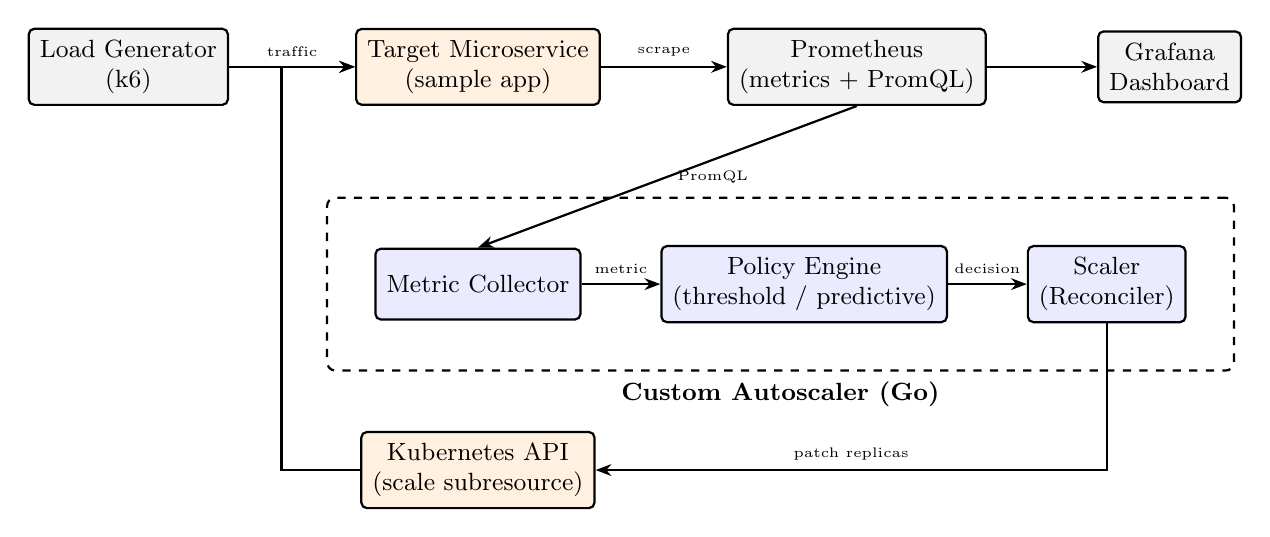
\begin{tikzpicture}[
  node distance=8mm,
  box/.style={draw, rounded corners=2pt, align=center, minimum height=9mm,
              inner sep=4pt, font=\small},
  ext/.style={box, fill=black!5},
  core/.style={box, fill=blue!8},
  app/.style={box, fill=orange!12},
  >={Stealth[length=2mm]},
  every path/.style={->, thick}
]
  \node[ext]  (lg)   {Load Generator\\(k6)};
  \node[app]  (app)  [right=16mm of lg] {Target Microservice\\(sample app)};
  \node[ext]  (prom) [right=16mm of app] {Prometheus\\(metrics + PromQL)};
  \node[ext]  (graf) [right=14mm of prom] {Grafana\\Dashboard};

  \node[core] (mc)   [below=18mm of app]  {Metric Collector};
  \node[core] (pe)   [right=10mm of mc]   {Policy Engine\\(threshold / predictive)};
  \node[core] (sc)   [right=10mm of pe]   {Scaler\\(Reconciler)};

  \node[app]  (api)  [below=14mm of mc]  {Kubernetes API\\(scale subresource)};

  \draw (lg)   -- node[above, font=\tiny] {traffic}  (app);
  \draw (app)  -- node[above, font=\tiny] {scrape}   (prom);
  \draw (prom) -- (graf);
  \draw (prom.south) -- node[right, font=\tiny] {PromQL} (mc.north);
  \draw (mc)   -- node[above, font=\tiny] {metric}   (pe);
  \draw (pe)   -- node[above, font=\tiny] {decision} (sc);
  \draw (sc.south) |- node[near end, above, font=\tiny] {patch replicas} (api.east);
  \draw (api.west) -- ++(-10mm,0) |- (app.west);

  \begin{scope}[on background layer]
    \node[draw, dashed, rounded corners=3pt, fit=(mc)(pe)(sc),
          inner sep=6mm, label={[font=\small\bfseries]below:Custom Autoscaler (Go)}] {};
  \end{scope}
\end{tikzpicture}%
}
\end{latin}
\caption[معماری سامانه]{معماری سامانه. مقیاس‌گذار سفارشی (کادر نقطه‌چین) سیگنال را از
\lr{Prometheus} می‌خواند، اندازه‌ی ناوگان را تصمیم می‌گیرد، و آن را از راه زیرمنبع
\lr{scale} اعمال می‌کند. سنجه‌های داخلی خود مقیاس‌گذار نیز به \lr{Prometheus} داده می‌شود.}
\label{fig:architecture}
\end{figure}

مؤلفه‌ها مطابق جدول~\ref{tab:design-components} به بسته‌های کد نگاشته می‌شوند:

\begin{table}[H]
\centering
\small
\caption[نگاشت مؤلفه‌های معماری به بسته‌های کد]{نگاشت مؤلفه‌های معماری به بسته‌ها و
 واسط‌های کد. همه‌ی بسته‌ها زیر \code{internal/} قرار دارند.}
\label{tab:design-components}
\scriptsize
\begin{tabular}{|l|l|l|l|}
\hline
\textbf{مؤلفه} & \textbf{بسته} & \textbf{واسط} & \textbf{پیاده‌سازی‌ها} \\
\hline
جمع‌آورنده‌ی سنجه & \code{metrics} & \code{Collector.Read} & \code{Prometheus}، \code{Static} \\
موتور سیاست & \code{policy} & \code{Policy.Decide} & \code{Threshold}، \code{PredictiveTotalLoad}، \\
 & & & \code{PredictivePerReplica} \\
پیش‌بینی‌کننده & \code{policy} & \code{Forecaster.Update} & \code{EWMATrend}، \code{Holt} \\
مقیاس‌گذار & \code{scaler} & \code{Scaler.Get} / \code{Set} & \code{Kubernetes}، \code{InMemory} \\
آشتی‌دهنده & \code{controller} & \lr{---} & حلقه‌ی کنترل \\
صادرکننده‌ی سنجه & \code{observability} & \lr{---} & نقطه‌ی \code{/metrics} \\
\hline
\end{tabular}
\end{table}

ورودی سامانه سنجه‌های سطح‌برنامه از \lr{Prometheus} است: نرخ درخواست، تأخیر، طول صف. این
سنجه‌ها از راه یک عبارت \lr{PromQL} خوانده می‌شوند که در پیکربندی تعیین می‌شود. خروجی سامانه
تعداد نمونه‌ی \lr{Deployment} هدف است، به‌علاوه‌ی سنجه‌های داخلی خود مقیاس‌گذار برای
مصورسازی در \lr{Grafana}.

\section{جمع‌آورنده‌ی سنجه}
\label{sec:design-collector}

جمع‌آورنده یک عبارت \lr{PromQL} را از پیکربندی می‌خواند و اجرا می‌کند. این عبارت در کد
سخت‌کد نشده است. همین نکته ادعای «مقیاس‌گذاری بر پایه‌ی سنجه‌های سطح‌برنامه» را از یک ادعای
کلی به یک قابلیت واقعی تبدیل می‌کند. نرخ درخواست، تأخیر یا طول صف تنها با تغییر یک رشته در
فایل پیکربندی جای یکدیگر را می‌گیرند و کد دست‌نخورده می‌ماند.

عبارتی که در ارزیابی به کار رفت:

\begin{latin}
\begin{lstlisting}[language=promql]
sum(rate(http_requests_total{app="sample"}[1m]))
  / clamp_min(count(up{app="sample"} == 1), 1)
\end{lstlisting}
\end{latin}

در همین عبارت کوتاه دو تصمیم طراحی نهفته است. نخست آنکه مخرج، تعداد نمونه‌هایی است که
\lr{Prometheus} آن‌ها را در دسترس می‌بیند و نه \lr{spec.replicas}. این انتخاب سیگنال را با
پایه‌ی «نمونه‌ی آماده» هم‌خوان نگه می‌دارد که سیاست به کار می‌برد و در
بخش~\ref{sec:design-formula} توضیح داده می‌شود. دوم آنکه \lr{clamp\_min} جلوی تقسیم بر صفر را
می‌گیرد، برای لحظه‌ای که هیچ نمونه‌ای آماده نیست.

نکته‌ی سومی نیز هست که در فصل~\ref{ch:results} اهمیت پیدا می‌کند: صورت کسر یک \lr{sum} روی
\emph{همه‌ی} سری‌هاست و مخرج تعداد هدف‌های در دسترس را می‌شمارد. پس هیچ‌یک از دو طرف به این
وابسته نیست که \emph{کدام} نمونه‌ها ترافیک گرفته‌اند. همین ویژگی است که باعث می‌شود نقص تحویل
بارِ توضیح‌داده‌شده در بخش~\ref{sec:results-loaddefect}، ورودی مقیاس‌گذار را خراب نکند.

رفتار در خطا هم صریح است. اگر خواندن سنجه ناموفق بماند، جمع‌آورنده خطا برمی‌گرداند و حلقه‌ی
کنترل تعداد نمونه‌ی فعلی را نگه می‌دارد. منطق این تصمیم ساده است: نبود سنجه شاهدی بر تغییر بار
در هیچ‌یک از دو جهت نیست، پس امن‌ترین کار هیچ‌کاری‌نکردن است.

پیاده‌سازی دوم این واسط، \code{Static}، مقداری ثابت یا دنباله‌ای از پیش تعیین‌شده برمی‌گرداند
و همان چیزی است که آزمون‌های حلقه‌بسته را ممکن می‌کند.

\section{موتور سیاست}
\label{sec:design-policy}

\subsection{فرمول پایه: نمونه‌های آماده، نه نمونه‌های درخواست‌شده}
\label{sec:design-formula}

تعداد نمونه‌ی هدف از همان فرمولی می‌آید که \lr{HPA} به کار می‌برد
(برابری~\ref{eq:hpa} در فصل~\ref{ch:background}):

\begin{equation}
\label{eq:desired}
d = \left\lceil r \times \frac{m}{T} \right\rceil
\end{equation}

که در آن $r$ تعداد نمونه‌های آماده، $m$ سنجه‌ی مشاهده‌شده و $T$ نرخ هدف است.

نکته‌ی ظریف در انتخاب پایه است. نمونه‌ی اولیه‌ی پایتونی این پروژه \lr{spec.replicas} را در
فرمول می‌گذاشت، در حالی که سنجه به‌ازای هر نمونه‌ی \emph{آماده} اندازه گرفته می‌شد. این دو در
حالت پایدار یکی هستند اما تا وقتی نمونه‌های تازه در حال آماده‌شدن‌اند از هم واگرا می‌شوند.
همان بازه، دقیقاً پنجره‌ای است که در یک مقیاس‌گیری به بالا اهمیت دارد.

یک مثال عددی کافی است، که اکنون به شکل آزمون \code{TestFormulaBaseIsReadyNotSpec} تثبیت شده
است. فرض کنید $\mathrm{spec} = 4$، $r = 2$، $m = 200$ و $T = 100$. پاسخ درست ۴ است. اگر
\lr{spec} را پایه بگیریم پاسخ ۸ می‌شود، یعنی دو برابر. مقیاس‌گذار بار مشاهده‌شده را بر
نمونه‌هایی تقسیم می‌کند که درخواست کرده، نه نمونه‌هایی که واقعاً سرویس می‌دهند. پس
بیش‌ازاندازه مقیاس می‌گیرد.

به همین دلیل \code{Scaler} هر دو عدد را برمی‌گرداند و سیاست از \code{Ready} استفاده می‌کند.
این یک بهبود عمدی نسبت به نمونه‌ی اولیه است و نه صرفاً ترجمه‌ی آن.

نکته‌ی متقارن آن هم اهمیت دارد. تصمیم \emph{اعمال} با \lr{spec.replicas} مقایسه می‌شود و نه
با \lr{ready}. پرسش آن مرحله این است که آیا پیش‌تر همین تعداد از خوشه خواسته شده است یا نه.
نمونه‌هایی که هنوز بالا می‌آیند، خواسته شده‌اند. اگر با \lr{ready} مقایسه می‌کردیم، همان
مقیاس‌گیری به بالا در هر چرخه دوباره صادر می‌شد تا وقتی نمونه‌ها بالا بیایند.

\subsection{ناحیه‌ی مرده}
\label{sec:design-deadband}

مانند \lr{HPA}، تغییری اعمال نمی‌شود مگر آنکه نسبت $m/T$ بیش از یک آستانه‌ی نسبی $\varepsilon$
از یک فاصله بگیرد:

\begin{equation}
\label{eq:deadband}
\left| \frac{m}{T} - 1 \right| \le \varepsilon \;\Longrightarrow\; d = r
\end{equation}

این آستانه به‌صورت پیش‌فرض ۱۰ درصد است. ناحیه‌ی مرده جلوی تعقیب نوسان‌های کوچک سنجه را
می‌گیرد.

مرز دقیق این ناحیه عمداً در هیچ آزمونی تثبیت نشده است. دلیلش رفتار ممیز شناور است. مثلاً
\lr{110/100} برابر \lr{1.1000000000000001} ارزیابی می‌شود، پس $|m/T - 1|$ اندکی از ۱۰ درصد
بزرگ‌تر می‌شود و ناوگان حرکت می‌کند. جفت دیگری از سنجه و هدف با همان نسبت اسمی ممکن است
آن‌سوی مرز بیفتد و ثابت بماند. \lr{HPA} استاندارد نیز همین نسبت را به همین شکل حساب می‌کند و
همین ابهام را به ارث می‌برد. اگر این مرز را در آزمون تثبیت می‌کردیم، به‌جای یک تصمیم طراحی،
مصنوعی از نمایش دودویی اعداد را تثبیت کرده بودیم.

\subsection{سیاست آستانه‌ای}
\label{sec:design-threshold}

ساده‌ترین سیاست است. سنجه‌ی جاری را در فرمول~\ref{eq:desired} می‌گذارد و تعداد نمونه را
پیشنهاد می‌دهد. این سیاست کاملاً واکنشی است و در ارزیابی نقش خط مبنا را دارد. ارزش افزوده‌ی
پیش‌بینی در برابر همین خط سنجیده می‌شود.

\subsection{پیش‌بینی‌کننده‌ها}
\label{sec:design-forecasters}

دو پیش‌بینی‌کننده پشت واسط \code{Forecaster} پیاده‌سازی شده است. هر دو حالت‌دار و ارزان‌اند،
چون در هر چرخه‌ی کنترل یک بار فراخوانی می‌شوند.

\textbf{\code{EWMATrend}} \mdash{} پیش‌فرض پیکربندی. سری را با میانگین متحرک نمایی هموار می‌کند و
سپس اختلاف دو مقدار هموارشده‌ی متوالی را به‌عنوان برآورد شیب می‌گیرد و به‌صورت خطی برون‌یابی
می‌کند:

\begin{align}
\label{eq:ewmatrend}
\ell_k &= \alpha\, x_k + (1-\alpha)\, \ell_{k-1} \\
\hat{x}_{k+h} &= \max\!\left(0,\; \ell_k + h\,(\ell_k - \ell_{k-1})\right)
\end{align}

\textbf{\code{Holt}} \mdash{} هموارسازی نمایی مضاعف مطابق برابری~\ref{eq:holt}، که سطح و شیب را با
دو ضریب جداگانه نگه می‌دارد و بنابراین یک روند پایدار را به اندازه‌ی \code{EWMATrend} میرا
نمی‌کند.

دو نکته‌ی پیاده‌سازی در هر دو مشترک است. نخست، کف \emph{نامنفی} روی خروجی: پیش‌بینی منفی برای
نرخ ورود درخواست بی‌معناست و \mdash{} چنان‌که در بخش~\ref{sec:design-defects} می‌آید \mdash{} اگر به
فرمول برسد به یک مقیاس‌گیری به پایینِ ناشی از نقص اندازه‌گیری می‌انجامد. دوم، مسیر جداگانه‌ای
برای ورودی \lr{NaN} یا بی‌نهایت، که در عمل یعنی یک \lr{scrape} ازدست‌رفته.

پیش‌بینی‌کننده‌ی دوم صرفاً برای آن هست که نشان دهد روش پیش‌بینی واقعاً افزون‌پذیر است و در
واسط قفل نشده. این همان ادعایی است که در نیازمندی‌های کارکردی آمده بود: پشتیبانی از سیاست‌های
چندگانه و پیکربندی‌پذیر، بدون تغییر در کد.

\subsection{سیاست پیش‌بینانه}
\label{sec:design-predictive}

سیاست پیش‌بینانه به‌جای مقدار جاری، مقدار پیش‌بینی‌شده برای چند گام بعد را در فرمول می‌گذارد.
فاصله‌ی آشتی‌دهی ۱۵ ثانیه و افق ۳ گام است، پس حدود ۴۵ ثانیه زمان پیش‌دستی به دست می‌آید. این
بازه تقریباً هم‌اندازه‌ی زمان آماده‌شدن یک نمونه‌ی جدید است و همین است که پیش‌بینی را سودمند
می‌کند.

\subsection{پیش‌بینی بار کل در برابر بار هر نمونه}
\label{sec:design-perreplica}

این بخش هسته‌ی علمی پروژه است. تصمیمی را ثبت می‌کند که از اندازه‌گیری به دست آمد و نه از
مطالعه‌ی کد.

نمونه‌ی اولیه بار \emph{هر نمونه} را پیش‌بینی می‌کرد. اما بار هر نمونه برابر است با بار کل
تقسیم بر نمونه‌های آماده،

\begin{equation}
\label{eq:perreplica}
m(t) = \frac{\lambda(t)}{r(t)}
\end{equation}

و $r(t)$ همان کمیتی است که مقیاس‌گذار تعیین می‌کند. پس پیش‌بینی‌کننده سیگنالی را برون‌یابی
می‌کند که کنش‌های خودش آن را جابه‌جا می‌کند. حلقه بهره‌ی مثبت پیدا می‌کند، مطابق آنچه
شکل~\ref{fig:feedback} نشان می‌دهد.

\begin{figure}[H]
\centering
\begin{latin}
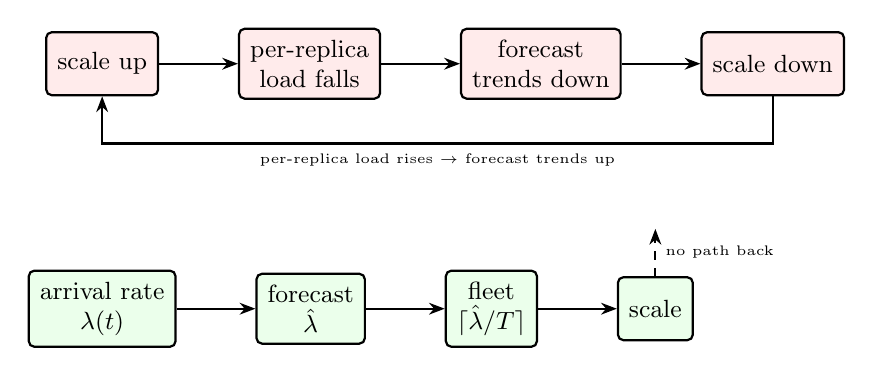
\begin{tikzpicture}[
  node distance=6mm,
  n/.style={draw, rounded corners=2pt, align=center, font=\small,
            minimum height=8mm, inner sep=4pt},
  bad/.style={n, fill=red!8},
  good/.style={n, fill=green!8},
  >={Stealth[length=2mm]},
  every path/.style={->, thick}
]
  % --- unstable loop
  \node[bad] (a) {scale up};
  \node[bad] (b) [right=10mm of a] {per-replica\\load falls};
  \node[bad] (c) [right=10mm of b] {forecast\\trends down};
  \node[bad] (d) [right=10mm of c] {scale down};

  \draw (a) -- (b);
  \draw (b) -- (c);
  \draw (c) -- (d);
  \draw (d.south) -- ++(0,-6mm) -| node[near start, below, font=\tiny]
        {per-replica load rises $\rightarrow$ forecast trends up} (a.south);

  % --- stable loop
  \node[good] (e) [below=22mm of a] {arrival rate\\$\lambda(t)$};
  \node[good] (f) [right=10mm of e] {forecast\\$\hat{\lambda}$};
  \node[good] (g) [right=10mm of f] {fleet\\$\lceil \hat{\lambda}/T \rceil$};
  \node[good] (h) [right=10mm of g] {scale};

  \draw (e) -- (f);
  \draw (f) -- (g);
  \draw (g) -- (h);
  \draw[dashed, ->] (h.north) -- node[right, font=\tiny] {no path back} ++(0,6mm);
\end{tikzpicture}
\end{latin}
\caption[پس‌خور مثبت در پیش‌بینی بار هر نمونه]{بالا: پیش‌بینی بار هر نمونه یک مسیر بسته با
بهره‌ی مثبت می‌سازد. پایین: پیش‌بینی نرخ ورود، که برون‌زاست، چنین مسیری ندارد و اندازه‌ی
ناوگان به تعداد نمونه‌ی جاری وابسته نیست.}
\label{fig:feedback}
\end{figure}

\textbf{چرا سیاست واکنشی روی همین سیگنال پایدار می‌ماند.} پرسش طبیعی این است که سیاست
آستانه‌ای هم همین $m$ درون‌زا را می‌خواند، پس چرا نوسان نمی‌کند. پاسخ در جبر فرمول پایه
است: وقتی $m$ بی‌واسطه در برابری~\ref{eq:desired} بنشیند، $r$ دقیقاً حذف می‌شود.

\begin{equation}
\label{eq:cancel}
d = \left\lceil r \times \frac{m}{T} \right\rceil
  = \left\lceil r \times \frac{\lambda/r}{T} \right\rceil
  = \left\lceil \frac{\lambda}{T} \right\rceil
\end{equation}

یعنی تصمیم سیاست واکنشی اصلاً تابع $r$ نیست، هرچند سیگنالش درون‌زاست. پس درون‌زا بودن سیگنال
به‌خودی‌خود مشکل‌ساز نیست؛ مشکل آنجاست که این حذف‌شدن به هم بخورد.

و پیش‌بینی‌کننده دقیقاً همین کار را می‌کند، چون یک عملگر \emph{حافظه‌دار} است که میان تقسیم
بر $r$ و ضرب در $r$ می‌نشیند: مقدار $\hat{x}_{k+h}$ از تاریخچه‌ی هموارشده‌ی
$m_j = \lambda_j / r_j$ برای $j \le k$ ساخته می‌شود، اما در برابری~\ref{eq:desired} در
$r_k$ \emph{جاری} ضرب می‌شود، و آن $r_j$های گذشته با $r_k$ حذف نمی‌شوند.

اثر را زیر بار کل \emph{ثابت} می‌توان دید. با $\lambda$ ثابت و برابری~\ref{eq:ewmatrend}:

\begin{equation}
\label{eq:gain}
\ell_k - \ell_{k-1} = \alpha\left( \frac{\lambda}{r_k} - \ell_{k-1} \right)
\end{equation}

تنها محرک شیب برآوردشده، تغییر خود $r$ است؛ بار اصلاً تکان نخورده. این شیب سپس در افق $h$
ضرب و به پیش‌بینی افزوده می‌شود، پس $h$ همان دستگیره‌ی بهره‌ی حلقه است و انتظار می‌رود افق
بلندتر ناپایداری را تندتر کند. جدول~\ref{tab:design-oscillation-unit} همین را زیر بار ثابت
نشان می‌دهد.

راه حل، پیش‌بینی بار کل است. \code{PredictiveTotalLoad} نرخ کل ورود درخواست‌ها را از حاصل‌ضرب
$m \times r$ بازسازی می‌کند، همان را پیش‌بینی می‌کند، و ناوگان را چنین اندازه می‌گیرد:

\begin{equation}
\label{eq:fleetfor}
d = \left\lceil \frac{\hat{\lambda}_{k+h}}{T} \right\rceil
\end{equation}

نرخ کل ورود درخواست‌ها یک ورودی \emph{برون‌زا} است، چون مقیاس‌گذار نمی‌تواند تعداد درخواست‌های
کاربران را تغییر دهد. پس بهره‌ی این مسیر ساختاراً صفر است: در
برابری~\ref{eq:fleetfor} هیچ وابستگی‌ای به $r$ دیده نمی‌شود. اینجا ضرب و تقسیم در
\emph{یک چرخه} انجام می‌شوند، پس برخلاف حالت پیش‌بینی بار هر نمونه، هیچ $r$ قدیمی وارد
حاصل نمی‌شود. تنها باقی‌مانده‌ی جزئی از آنجاست که مخرج جمع‌آورنده \code{count(up)} است و
ضریب بازسازی \code{status.readyReplicas}؛ این دو منبع متفاوت‌اند و در گذراها می‌توانند
اندکی از هم فاصله بگیرند. این نکته، تفاوت میان دو سیاست را از یک مشاهده‌ی تجربی به یک ویژگی
ساختاری ارتقا می‌دهد.

اثر را در حلقه‌ی بسته و مستقل از هر زیرساختی اندازه گرفتیم، در آزمون
\code{TestPerReplica\-Forecasting\-Oscillates\-Under\-ConstantLoad}. بار کل ثابت ۵۰۰ درخواست بر ثانیه
بود، هدف ۱۰۰، پیش‌بینی‌کننده \lr{EWMA} با افق ۳ و $\alpha$ برابر ۰/۵. چهل گام اجرا شد که ده
گام نخست آن به عنوان شیب اولیه کنار گذاشته شد. سازوکار پایدارسازی خاموش بود.

\begin{table}[H]
\centering
\caption{نوسان تحت بار کل \emph{ثابت}، در آزمون واحد حلقه‌بسته}
\label{tab:design-oscillation-unit}
\small
\begin{tabular}{|l|c|l|}
\hline
\textbf{سیاست} & \textbf{تغییر تعداد نمونه در ۳۰ گام پایدار} & \textbf{ناوگان} \\
\hline
\code{PredictiveTotalLoad} & \textbf{0} & روی ۵ می‌نشیند و تکان نمی‌خورد \\
\code{PredictivePerReplica} & \textbf{29} & میان ۱ و ۸ نوسان می‌کند \\
\hline
\end{tabular}
\end{table}

خاموش‌بودن سازوکار پایدارسازی در این آزمون عمدی است. آن سازوکار یک میراگر است، و میراکردن
نشانه همان ویژگی‌ای را پنهان می‌کند که موضوع آزمون است. ناپایداری در دینامیک خود سیاست
زندگی می‌کند و نه در خروجی میراشده‌ی آن.

همین پدیده در شبیه‌ساز هم دیده می‌شود، این بار با پیکربندی کامل و بار کاری \arm{spike}:

\begin{table}[H]
\centering
\caption{همان پدیده در شبیه‌ساز، با پیکربندی کامل}
\label{tab:design-oscillation-sim}
\begin{tabular}{|l|c|l|l|}
\hline
\textbf{سیاست} & \textbf{تغییر تعداد نمونه} & \textbf{هزینه} & \textbf{نقض \lr{SLA}} \\
\hline
\code{Threshold} & 4 & مبنا & مبنا \\
\code{PredictivePerReplica} & \textbf{17} & ‎+۲۳ درصد & یکسان \\
\code{PredictiveTotalLoad} & \textbf{3} & برابر \code{Threshold} & بهتر روی \arm{diurnal} \\
\hline
\end{tabular}
\end{table}

بیست‌وسه درصد هزینه‌ی بیشتر، آن هم بدون هیچ سودی در کیفیت خدمت. تیزترین بیان شکست شکل «هر
نمونه» همین است: روی هر دو محور اکیداً بدتر است.

باید تأکید کرد که ارقام جدول‌های~\ref{tab:design-oscillation-unit}
و~\ref{tab:design-oscillation-sim} \emph{قابل تعویض با یکدیگر نیستند}. ارقام آزمون واحد
می‌گویند خود سیاست به‌تنهایی چه می‌کند؛ ارقام شبیه‌ساز می‌گویند پیکربندی کامل چه می‌کند. هر
دو در ارزیابی جای دارند، به شرط آنکه برچسب‌گذاری شوند.

\code{PredictivePerReplica} عمداً در کد باقی مانده. تقابل این دو خودش یک نتیجه‌ی ارزیابی است
و نه کد مرده. برای آنکه به‌اشتباه به‌عنوان سیاست عملیاتی انتخاب نشود، هنگام گزینش آن یک
هشدار در گزارش‌ها ثبت می‌شود.

\section{سازوکار پایدارسازی}
\label{sec:design-stabilizer}

این سازوکار پاسخ پیاده‌سازی به نیازمندی غیرکارکردی «پرهیز از نوسان» است و سه بخش دارد.

\textbf{نخست، پنجره‌ی پایدارسازی نامتقارن.} مقیاس‌گیری به بالا بی‌درنگ اعمال می‌شود، چون کندی
در افزودن ظرفیت مستقیماً به تأخیر کاربر تبدیل می‌شود. مقیاس‌گیری به پایین اما بر پایه‌ی
\emph{بیشینه‌ی} پیشنهادهای دیده‌شده در طول پنجره‌ی $W$ تصمیم گرفته می‌شود:

\begin{equation}
\label{eq:stabilize}
d_{\mathrm{applied}} =
\begin{cases}
d_k & d_k > r \quad\text{(مقیاس به بالا، بی‌درنگ)}\\[2mm]
\max\{\, d_j \;:\; t_k - W \le t_j \le t_k \,\} & d_k < r \quad\text{(مقیاس به پایین)}
\end{cases}
\end{equation}

مقدار پیش‌فرض $W$ برابر ۹۰ ثانیه است. به این ترتیب یک افت کوتاه بار نمی‌تواند ناوگان را کوچک
کند. خود \lr{Kubernetes} نیز در \lr{scaleDown.stabilizationWindowSeconds} همین رفتار را دارد.

\textbf{دوم، شیب‌گیری}\LTRfootnote{Cooldown}. حداقل فاصله‌ی زمانی میان دو کنش مقیاس‌گذاری.
این مؤلفه در نمونه‌ی اولیه نبود و در پیشنهاد پروژه نام برده شده بود. نکته‌ی مهم پیاده‌سازی آن
در بخش~\ref{sec:design-defects} می‌آید: شیب‌گیری باید \emph{به تفکیک جهت} باشد.

\textbf{سوم، سقف گام.} بیشینه‌ی تعداد نمونه‌ای که یک تصمیم منفرد می‌تواند اضافه یا کم کند.

در همه‌ی آزمایش‌های این نوشتار، شیب‌گیری و سقف گام غیرفعال بوده‌اند و تنها پنجره‌ی پایدارسازی
فعال بوده است. دلیل این انتخاب آن است که متغیر مورد مطالعه یکی بماند: هر سه مؤلفه میراگرند و
فعال‌بودن هم‌زمانشان سهم هرکدام را غیرقابل تفکیک می‌کند.

باید صریح گفت که این سازوکار یک \emph{میراگر} است و نه یک \emph{اصلاح}. فصل~\ref{ch:results}
نشان می‌دهد که همین میراگر می‌تواند یک قانون کنترل معیوب را چنان بپوشاند که از همه‌ی آزمون‌ها
سربلند بیرون بیاید. این خودش یکی از نتایج پروژه است.

\section{مقیاس‌گذار}
\label{sec:design-scaler}

مقیاس‌گذار تصمیم را از راه زیرمنبع \lr{scale} روی \lr{Deployment} هدف اعمال می‌کند، و تنها
وقتی که عدد نسبت به \lr{spec.replicas} تغییر کرده باشد.

یک تصمیم پیاده‌سازی در اینجا ارزش ثبت دارد. عملیات \code{Get} از زیرمنبع \lr{scale} استفاده
\emph{نمی‌کند} و به‌جای آن یک بار خودِ \lr{Deployment} را می‌خواند. دلیلش آن است که زیرمنبع
\lr{scale} نمی‌تواند به پرسش دوم پاسخ دهد: وضعیت آن تعداد \emph{کل} نمونه‌ها را گزارش می‌کند
و نه تعداد نمونه‌های \emph{آماده} را، حال آنکه فرمول به عدد دوم نیاز دارد. خواندن یک‌باره‌ی
\lr{Deployment} هر دو عدد را می‌دهد و تعداد فراخوانی واسط برنامه‌نویسی را در هر چرخه نصف
می‌کند. عملیات \code{Set} همچنان از \lr{GetScale} و \lr{UpdateScale} استفاده می‌کند تا
چرخه‌ی خواندن-تغییر-نوشتن روی \lr{resourceVersion} درست انجام شود.

پیاده‌سازی دوم این واسط، یعنی \code{InMemory}، همان است که آزمون‌های حلقه‌بسته‌ی
بخش~\ref{sec:design-perreplica} را ممکن می‌کند.

\section{مشاهده‌پذیری}
\label{sec:design-observability}

مقیاس‌گذار سنجه‌های داخلی خودش را روی یک نقطه‌ی \lr{/metrics} منتشر می‌کند. مهم‌ترین آن‌ها در
جدول~\ref{tab:design-metrics} آمده است.

\begin{table}[H]
\centering
\small
\caption{سنجه‌های داخلی منتشرشده توسط مقیاس‌گذار}
\label{tab:design-metrics}
\begin{tabular}{|l|l|}
\hline
\textbf{نام سنجه} & \textbf{معنا} \\
\hline
\code{autoscaler\_current\_replicas} & تعداد نمونه‌ی درخواست‌شده (\lr{spec.replicas}) \\
\code{autoscaler\_ready\_replicas} & تعداد نمونه‌ی آماده؛ پایه‌ی فرمول \\
\code{autoscaler\_desired\_replicas} & تصمیم سیاست، پس از پایدارسازی \\
\code{autoscaler\_raw\_recommendation} & پیشنهاد خام، پیش از پایدارسازی \\
\code{autoscaler\_metric\_value} & مقدار مشاهده‌شده‌ی سیگنال \\
\code{autoscaler\_metric\_target} & نقطه‌ی هدف \\
\code{autoscaler\_predicted\_value} & مقدار پیش‌بینی‌شده (صفر برای سیاست‌های واکنشی) \\
\code{autoscaler\_reconcile\_duration\_seconds} & زمان اجرای هر چرخه \\
\code{autoscaler\_scale\_actions\_total} & شمار کنش‌های مقیاس‌گذاری \\
\code{autoscaler\_collector\_errors\_total} & خطاهای خواندن سنجه \\
\hline
\end{tabular}
\end{table}

این سنجه‌ها سه کاربرد دارند. یکی مصورسازی در \lr{Grafana}. دوم، پایش سلامت خود مقیاس‌گذار.
سوم \mdash{} و مهم‌ترین برای این نوشتار \mdash{} یک \emph{بررسی اعتبار مستقل}. تفاوت میان
\code{autoscaler\_raw\_recommendation} و \code{autoscaler\_desired\_replicas} دقیقاً می‌گوید
میراگر چه مقدار کار انجام داده است؛ و مقایسه‌ی \code{autoscaler\_metric\_value} با بار
مشاهده‌شده‌ی هر نمونه، امضای پس‌خور مثبت را آشکار می‌کند. در
بخش~\ref{sec:results-stabilizer} از هر دو استفاده شده است.

یک تصمیم کوچک اما آگاهانه: نام سنجه‌ها پیشوند \code{autoscaler\_} را نگه داشته‌اند، هرچند نام
پروژه به \lr{setpoint} تغییر کرده است. تغییر نام یک سنجه، هر پنل \lr{Grafana} و هر شکل
فصل ارزیابی را بی‌اعتبار می‌کند. یک آزمون این نام‌ها را تثبیت کرده است.

\section{حلقه‌ی کنترل}
\label{sec:design-loop}

هر \lr{interval\_seconds} یک چرخه‌ی آشتی‌دهی اجرا می‌شود. مقدار پیش‌فرض ۱۵ ثانیه است که با
دوره‌ی همگام‌سازی \lr{HPA} هم‌اندازه است. هر چرخه شش گام دارد:

\begin{enumerate}
  \item خواندن سیگنال مقیاس‌گذاری از \lr{Prometheus} با \lr{PromQL}.
  \item خواندن \lr{spec.replicas} و \lr{status.readyReplicas} از هدف.
  \item گرفتن پیشنهاد خام از سیاست.
  \item پایدارسازی: مقیاس به بالا بی‌درنگ، مقیاس به پایین مشروط به بیشینه‌ی پنجره، سپس سقف
  گام و شیب‌گیری.
  \item اعمال از راه زیرمنبع \lr{scale}، در صورت تغییر عدد.
  \item صدور تصمیم و ورودی‌هایش روی \lr{/metrics}.
\end{enumerate}

شکست در هر گام ثبت می‌شود و تعداد نمونه‌ی جاری نگه داشته می‌شود. این انتخاب \mdash{} «نگه‌داشتن» به
جای «حدس زدن» \mdash{} تنها پاسخ امن به نبود اطلاعات است: قطعی \lr{Prometheus} شاهدی بر بالا رفتن یا
پایین آمدن بار نیست.

\textbf{سربار خود مقیاس‌گذار.} در یک اجرای واقعی، ۱۸ چرخه‌ی آشتی‌دهی مجموعاً ۰/۰۶۸ ثانیه طول
کشید، یعنی حدود ۳/۸ میلی‌ثانیه بر چرخه در برابر یک فاصله‌ی ۱۵ ثانیه‌ای. حلقه‌ی کنترل به هیچ
وجه گلوگاه نیست، و این عدد پاسخ روشنی به پرسش «آیا زمان واکنش اندازه‌گیری‌شده‌ی شما صرفاً
کندی کنترل‌گر خودتان نیست؟» می‌دهد. این همان نیازمندی غیرکارکردی «سربار منابع پایین» است.

یک حالت \lr{dry-run} نیز پیاده‌سازی شده که تصمیم‌ها را ثبت می‌کند اما اعمال نمی‌کند. کاربرد
آن، اجرای مقیاس‌گذار در کنار یک سرویس واقعی برای دیدن اینکه \emph{چه می‌کرد} است، پیش از آنکه
اجازه‌ی نوشتن بگیرد.

\section{پیکربندی}
\label{sec:design-config}

کل رفتار سامانه از یک فایل \lr{YAML} می‌آید که در خوشه به شکل \lr{ConfigMap} نصب می‌شود. طرح
این فایل عمداً با فایل پیکربندی نمونه‌ی اولیه‌ی پایتونی یکی است. به این ترتیب مقایسه‌ی
شبیه‌ساز و خوشه در فصل~\ref{ch:results} با تفاوت تنظیمات مخدوش نمی‌شود.

جدول~\ref{tab:design-config} مقادیری را نشان می‌دهد که در همه‌ی اندازه‌گیری‌ها به کار رفت.
فایل کامل در پیوست الف آمده است.

\begin{table}[H]
\centering
\small
\caption{پیکربندی به‌کاررفته در همه‌ی اجراهای ارزیابی}
\label{tab:design-config}
\begin{tabular}{|l|c|l|}
\hline
\textbf{کلید} & \textbf{مقدار} & \textbf{توضیح} \\
\hline
\code{interval\_seconds} & 15 & هم‌اندازه‌ی دوره‌ی همگام‌سازی \lr{HPA} \\
\code{policy.target} & 100.0 & درخواست بر ثانیه بر هر نمونه‌ی آماده \\
\code{policy.tolerance} & 0.10 & ناحیه‌ی مرده‌ی ۱۰ درصدی، مانند \lr{HPA} \\
\code{policy.min\_replicas} & 1 & \\
\code{policy.max\_replicas} & 20 & بنگرید به توضیح زیر \\
\code{forecaster.type} & \code{ewma} & \code{EWMATrend} \\
\code{forecaster.horizon} & 3 & ‏۳ × ۱۵ ثانیه = ۴۵ ثانیه پیش‌دستی \\
\code{forecaster.alpha} & 0.5 & \\
\code{stabilization\_window\_seconds} & 90 & صفر در بازوهای حذفی \\
\code{cooldown\_seconds} & 0 & غیرفعال \\
\code{max\_step} & 0 & غیرفعال \\
\hline
\end{tabular}
\end{table}

انتخاب عدد ۲۰ برای بیشینه‌ی نمونه خودش یک تصمیم ارزیابی است و نه یک عدد دلبخواه. همه‌ی چهار
الگوی بار در اوج به ۱۲۰۰ تا ۱۳۰۰ درخواست بر ثانیه می‌رسند، که در برابر هدف ۱۰۰ یعنی ۱۲ تا ۱۳
نمونه. اگر سقف ۱۰ می‌بود، \emph{همه‌ی} بازوهای خودکار در اوج به سقف می‌خوردند و هر کدام با ۱۰
نمونه و ۱۳۰ درخواست بر ثانیه بر نمونه کار می‌کردند \mdash{} یعنی همگی یکسان و بالای خط کیفیت خدمت.
آنگاه سنجه‌ی نقض کیفیت خدمت دقیقاً در همان نقطه‌ای که مقایسه بیشترین اهمیت را دارد، بازوها را
از هم تفکیک نمی‌کرد، و سیاست پیش‌بینانه به دلیلی که هیچ ربطی به سیاست ندارد بهتر از واکنشی به
نظر نمی‌رسید. ظرفیت گره محدودیت نبود: ۲۰ نمونه ۴ هسته از ۱۴ هسته‌ی گره را درخواست می‌کنند.

\section{نقص‌هایی که آزمون‌ها آشکار کردند}
\label{sec:design-defects}

سه نقص در مسیر کنترل با نوشتن آزمون پیدا شد و نه با خواندن کد. هر سه وقتی آشکار شدند که
رفتار مورد انتظار را ادعا کردیم و ادعا شکست خورد. هیچ‌کدام با مطالعه‌ی کد دیده نمی‌شد، و
نکته‌ی مشترک هر سه آن است که تنها در بدترین وضعیت خوشه فعال می‌شوند.

\textbf{نخست، \code{Holt.Update} روی مسیر \lr{NaN} پیش‌بینی منفی برمی‌گرداند.} بازگشت زودهنگام
برای \lr{NaN} و \lr{Inf}، کف \lr{math.Max(0, ...)} را رد می‌کرد که مسیر عادی اعمال می‌کند. با
تغذیه‌ی ۵۰۰، ۴۰۰، ۱۰۰، ۱۰ و سپس \lr{NaN} با افق ۳ و $\alpha = \beta = 0.5$، مقدار منفی ۴۵۰
اندازه‌گیری شد. \code{FleetFor} این عدد را بی‌سروصدا به \lr{min\_replicas} کف می‌زد. یعنی یک
مقیاس‌گیری به پایین که علتش یک \lr{scrape} ازدست‌رفته بود و نه نبود بار. در گزارش‌ها هم
کاملاً عادی به نظر می‌رسید.

\textbf{دوم، شیب‌گیری سراسری بود و نه به تفکیک جهت.} این رفتار با توضیح خود تابع در تناقض
بود، که گفته بود مقیاس به بالا بی‌درنگ اعمال می‌شود. با طرح پروژه هم در تناقض بود. پیامدش
این بود که پس از یک مقیاس به پایین، بازگشت بار نمی‌توانست مقیاس به بالای جبرانی را در تمام
مدت شیب‌گیری فعال کند. یعنی دقیقاً همان حالتی که انتظار کشیدن در آن به قیمت نقض کیفیت خدمت
تمام می‌شود. اکنون بر پایه‌ی جهت کلید خورده است.

\textbf{سوم، تبدیل \lr{int32(math.Ceil(...))} به رفتار وابسته به پیاده‌سازی تکیه داشت.}
مشخصه‌ی زبان \lr{Go} می‌گوید تبدیل اعشاری به صحیح، وقتی نتیجه در نوع مقصد نگنجد، موفق می‌شود
اما مقدار نتیجه وابسته به پیاده‌سازی است. پس یک پیشنهاد بسیار بزرگ ممکن است روی یک معماری به
\lr{MaxInt32} اشباع شود و روی معماری دیگر به عددی \emph{منفی} بپیچد. آنگاه \code{clamp} عدد
منفی را «کمتر از کمینه» می‌خواند و ناوگان را زیر بار شدید \emph{کوچک} می‌کند. بدترین پاسخ
ممکن، که تصادفی به دست آمده باشد. آزمون‌ها روی این میزبان \lr{arm64} در هر دو حالت سبز
می‌مانند و دقیقاً به همین دلیل یک نگهبان صریح لازم بود، چون کانتینر برای معماری‌ای ساخته
می‌شود که با معماری توسعه یکی نیست. تابع \code{ceilToReplicas} اکنون عمداً اشباع می‌کند.

\section{برنامه‌ی نمونه و بستر آزمایش}
\label{sec:design-sampleapp}

برای آنکه ارزیابی معنا داشته باشد، سرویس هدف باید واقعاً محدود به پردازنده باشد. سرویسی که
به‌جای محاسبه فقط بخوابد، زیر بار فزاینده مصرف پردازنده‌ی ثابتی نشان می‌دهد. آنگاه بازوی
\arm{hpa-cpu} هرگز واکنش نشان نمی‌دهد و خط مبنا به یک مترسک تبدیل می‌شود.

پس برنامه‌ی نمونه برای هر درخواست مقدار مشخصی پردازنده می‌سوزاند. این مقدار چنان کالیبره شده
که نمونه‌ای در نرخ هدف خود دقیقاً ۱۰۰ درصد درخواست پردازنده‌اش را مصرف کند. جزئیات این
کالیبراسیون و تأیید آن در خوشه در بخش~\ref{sec:method-calibration} آمده است.

برنامه‌ی نمونه سه سنجه منتشر می‌کند: شمارنده‌ی \code{http\_requests\_total}، بافه‌ی
\code{http\_request\_\-duration\_\-seconds}، و سنجه‌ی لحظه‌ای \code{http\_requests\_in\_flight}.
دو پارامتر محیطی نیز دارد که رفتار آن را تنظیم می‌کنند: \code{WORK\_CPU\_MS} برای مقدار
پردازش هر درخواست و \code{WORK\_MAX\_CONCURRENT} برای سقف هم‌زمانی.

بستر آزمایش شامل \lr{Prometheus} و \lr{Grafana} از چارت \lr{kube-prometheus-stack} است،
به‌علاوه‌ی یک \lr{ServiceMonitor} برای سرویس هدف و مولد بار \lr{k6}. در این بستر چند دام
خاموش وجود داشت که کشفشان زمان برد و ثبتشان ارزش دارد.

\textbf{\lr{targetLabels: [app]} روی \lr{ServiceMonitor} الزامی است.} عبارت \lr{PromQL} روی
برچسب \lr{app="sample"} انتخاب می‌کند، اما این برچسب روی \lr{Service} است و نه در سنجه‌هایی
که خود برنامه منتشر می‌کند. بدون ارتقای این برچسب، پرس‌وجو هیچ‌چیز را تطبیق نمی‌دهد، برداری
تهی برمی‌گرداند، و ناوگان روی \lr{min\_replicas} می‌نشیند. همه‌ی این‌ها هم کاملاً خاموش رخ
می‌دهد.

\textbf{\lr{serviceMonitorSelectorNilUsesHelmValues} به‌صورت پیش‌فرض \lr{true} است.} در این
حالت \lr{Prometheus} فقط \lr{ServiceMonitor}هایی را کشف می‌کند که برچسب انتشار \lr{Helm} را
دارند. نمونه‌های دست‌نویس بی‌هیچ توضیحی در هیچ گزارشی نادیده گرفته می‌شوند.

\textbf{\code{http\_requests\_total} تا پیش از نخستین درخواست وجود ندارد.} نتیجه‌ی تهی
پرس‌وجو پیش از هر ترافیکی، رفتار درست است و نه خط لوله‌ی خراب. همین نکته یکی از دلایل وجود
مرحله‌ی گرم‌کردن در چارچوب آزمایش است (بخش~\ref{sec:method-harness}).

\textbf{\lr{kubectl port-forward} نمی‌تواند به یک ناوگان بار بدهد.} این فرمان \emph{یک} نقطه‌ی
انتهایی را حل می‌کند و همان را نگه می‌دارد. هر آزمایشی از این راه، به ظرفیت یک نمونه محدود
می‌ماند در حالی که ناوگان زیر آن بزرگ می‌شود و بی‌استفاده می‌ماند \mdash{} و همه‌ی بازوها یکسان به
نظر می‌رسند چون هیچ‌کدام واقعاً بارگذاری نشده‌اند. به همین دلیل \lr{Service} از نوع
\lr{LoadBalancer} تعریف شده است.

\section{جمع‌بندی فصل}
\label{sec:design-summary}

سامانه در امتداد سه دغدغه‌ی مستقل شکسته شده و هر مرحله واسطی با دست‌کم دو پیاده‌سازی دارد.
این ساختار، آزمون حلقه‌بسته‌ی سیاست را بدون خوشه ممکن می‌کند و یافته‌ی مرکزی پروژه از همین
راه به دست آمد.

دو انحراف از نمونه‌ی اولیه هر دو با اندازه‌گیری توجیه شده‌اند. پایه‌ی فرمول باید نمونه‌های
آماده باشد. پیش‌بینی باید روی بار کل انجام شود و نه بار هر نمونه، و دلیل آن ساختاری است:
اندازه‌ی ناوگان در برابری~\ref{eq:fleetfor} به تعداد نمونه‌ی جاری وابسته نیست.

سازوکار پایدارسازی یک میراگر است و نه اصلاح. فصل~\ref{ch:results} نشان می‌دهد چه چیزی را
می‌پوشاند.

سه نقص مسیر کنترل تنها با نوشتن آزمون به‌مثابه‌ی مشخصه آشکار شدند. هر سه در شرایطی فعال
می‌شدند که خوشه در بدترین وضعیت خود است: یک \lr{scrape} ازدست‌رفته، بازگشت بار پس از یک
مقیاس به پایین، و بار شدید روی معماری دیگر.

\chapter{روش‌شناسی ارزیابی}
\label{ch:method}

این فصل می‌گوید نتایج فصل~\ref{ch:results} \emph{چگونه} به دست آمده‌اند. تفکیک آن از فصل
نتایج عمدی است: بیشتر ادعاهای یک ارزیابی تجربی نه با خودِ اعداد، بلکه با روشی که اعداد را
تولید کرده است زیر سؤال می‌رود.

ساختار فصل چنین است: نخست بستر آزمایش و کالیبراسیون آن، سپس بارهای کاری و بازوهای مقایسه،
سپس تعریف دقیق سنجه‌ها، و سرانجام چارچوب آزمایش با بررسی‌های اعتبار آن. بخش پایانی به
دام‌هایی می‌پردازد که خودِ چارچوب در جریان ساخته‌شدن از آن‌ها آموخت \mdash{} بخشی که در بیشتر
گزارش‌ها نوشته نمی‌شود اما بیشترین ارزش عملی را دارد.

\section{سه سطح ارزیابی}
\label{sec:method-levels}

ارزیابی در سه سطح انجام شد، همان‌گونه که در پیشنهاد پروژه آمده بود:

\begin{enumerate}
  \item \textbf{آزمون واحد} برای منطق موتور سیاست، مستقل از خوشه.
  \item \textbf{آزمون یکپارچه‌سازی} برای رفتار سامانه در خوشه‌ی واقعی.
  \item \textbf{آزمون کارایی و مقایسه} در برابر سازوکار پیش‌فرض \lr{Kubernetes}.
\end{enumerate}

بیشتر این فصل و فصل بعد به سطح سوم می‌پردازد، چون ادعاهای اصلی پروژه از آنجا برمی‌آید. اما
سطح نخست از نظر روش‌شناختی جایگاه ویژه‌ای دارد: چون واسط‌ها تفکیک شده‌اند، یک حلقه‌ی کنترل
\emph{بسته} کاملاً درون یک آزمون واحد اجرا می‌شود. آنجا هیچ نویزی از شبکه، زمان‌بندی یا
تأخیر جمع‌آوری وجود ندارد، پس هر نوسانی که دیده شود قطعاً از خود سیاست است. این همان چیزی
است که ادعای بخش~\ref{sec:design-perreplica} را از یک همبستگی به یک سازوکار ارتقا می‌دهد.

\section{بستر آزمایش}
\label{sec:method-testbed}

همه‌ی اندازه‌گیری‌ها روی یک خوشه‌ی تک‌گرهی \lr{Kubernetes} انجام شد. جدول~\ref{tab:method-env}
محیط مرجع را ثبت می‌کند.

\begin{table}[H]
\centering
\small
\caption{محیط مرجع اندازه‌گیری‌ها}
\label{tab:method-env}
\begin{tabular}{|l|l|}
\hline
\textbf{مؤلفه} & \textbf{نسخه} \\
\hline
\lr{Go} & \lr{1.26.4} \\
\lr{kubectl} & \lr{v1.36.1} \\
\lr{Kubernetes} (\lr{Docker Desktop}) & \lr{v1.36.1}، تک‌گره \\
\lr{Kubernetes} (\lr{kind}) & \lr{v1.36.1}، سه‌گره \\
\lr{Helm} & \lr{v4.2.0} \\
\lr{kind} & \lr{v0.32.0} \\
\lr{k6} & \lr{v2.1.0} \\
\lr{kube-prometheus-stack} & \lr{prometheus-operator v0.92.1} \\
\lr{Prometheus Adapter} & \lr{v0.12.0} \\
تصویر پایه & \lr{golang:1.26-alpine} (ساخت)، \lr{distroless/static-debian12} (اجرا) \\
\textbf{تصویر برنامه‌ی نمونه} & \textbf{\lr{sha256:d089f870ba7a...}}، تثبیت‌شده با برچسب \\
 & \lr{sample-app:phase6-measured} \\
\hline
میزبان & \lr{macOS} (\lr{Darwin 25.5.0})، \lr{arm64} \\
ماشین مجازی & ۱۴ هسته، ۷/۷۴۹ گیگابایت حافظه، ۱۱۰ جایگاه \lr{Pod} \\
\hline
\end{tabular}
\end{table}

\lr{Prometheus} با فاصله‌ی جمع‌آوری سراسری ۱۵ ثانیه پیکربندی شد، اما برای دو
\lr{ServiceMonitor} که در اندازه‌گیری نقش دارند این فاصله ۵ ثانیه است. پنجره‌ی همه‌ی
پرس‌وجوهای \lr{rate} برابر یک دقیقه است.

سطر آخر جدول اهمیت ویژه‌ای دارد و در بخش~\ref{sec:results-image} به آن بازمی‌گردیم: تصویر
برنامه‌ی نمونه با اثرانگشت تثبیت شده است، چون یک برچسب تصویر قابل تغییر است و «همان برچسب»
تضمین «همان تصویر» نیست.

\subsection{چرا خوشه‌ی تک‌گره}
\label{sec:method-singlenode}

پیشنهاد پروژه \lr{k3s} یا \lr{kind} را نام برده بود، در حالی که توسعه‌ی روزانه روی
\lr{Kubernetes} داخلی \lr{Docker Desktop} انجام شد. این یک انحراف است و به‌جای آنکه صرفاً
ثبت شود، جبران شده است: یک پیکربندی سه‌گره‌ی \lr{kind} در مخزن قرار دارد و کل مسیر روی آن نیز
راستی‌آزمایی شده است \mdash{} سه گره آماده، هر دو تصویر بارگذاری‌شده، پخش نمونه‌ها میان دو گره کارگر،
دقیقاً یک هدف جمع‌آوری به ازای هر نمونه، و بازگرداندن یک \lr{kubectl scale} دستی توسط
مقیاس‌گذار.

با این حال، اندازه‌گیری‌های گزارش‌شده روی خوشه‌ی تک‌گره انجام شده‌اند. دلیل آن، حذف یک متغیر
مزاحم است: روی چند گره، رقابت زمان‌بندی و تفاوت بار گره‌ها به نتایج نویز اضافه می‌کند بی‌آنکه
به پرسش پژوهش ربطی داشته باشد. پیامد این انتخاب برای اعتبار نتایج در
بخش~\ref{sec:results-otherlimits} صریحاً گزارش شده است.

\section{کالیبراسیون برنامه‌ی نمونه}
\label{sec:method-calibration}

انصاف مقایسه به یک تساوی ساده وابسته است. برنامه‌ی نمونه برای هر درخواست حدود ۲ میلی‌ثانیه
پردازنده می‌سوزاند و درخواست منابع هر نمونه ۲۰۰ میلی‌کور است. پس:

\begin{equation}
\label{eq:calibration}
100~\mathrm{req/s} \times 2~\mathrm{ms} = 200~\mathrm{ms/s} = 200\mathrm{m}
\end{equation}

یعنی نمونه‌ای که در نرخ هدف خود کار می‌کند، دقیقاً ۱۰۰ درصد درخواست پردازنده‌اش را مصرف
می‌کند.

اهمیت این تساوی در آن است که دو بازو را به \emph{یک نقطه‌کار} می‌رساند. بازوی \arm{hpa-cpu}
روی \lr{averageUtilization: 100} تنظیم شده و بازوی \arm{ours-threshold} روی نرخ هدف ۱۰۰
درخواست بر ثانیه. بدون این تساوی، این دو به دو نقطه‌ی متفاوت نشانه می‌رفتند و هیچ تفاوتی
میانشان قابل انتساب نبود. تنظیم متعارف \lr{averageUtilization: 70} این تساوی را بی‌سروصدا
می‌شکست.

تساوی را اندازه گرفتیم و به استدلال اکتفا نکردیم. نخست روی میزبان و به‌صورت متوالی با
\lr{GOMAXPROCS=1}:

\begin{table}[H]
\centering
\caption{کالیبراسیون محلی برنامه‌ی نمونه}
\label{tab:method-calib-local}
\begin{tabular}{|l|r|r|}
\hline
\textbf{کمیت} & \textbf{اندازه‌گیری‌شده} & \textbf{انتظار} \\
\hline
تأخیر هر درخواست & \lr{2.096 ms} & \lr{2 ms} + سربار \lr{HTTP} \\
گذردهی تک‌هسته & \lr{477 req/s} & $\approx$\lr{500} \\
پردازنده‌ی ضمنی در \lr{100 req/s} & \lr{210m} & \lr{200m} \\
بازبینی با \lr{?cpu\_ms=8} & \lr{8.111 ms} & ۴ برابر حالت ۲ میلی‌ثانیه \\
\hline
\end{tabular}
\end{table}

سپس درون خوشه، با نگه داشتن بار روی یک نمونه و خواندن مصرف پردازنده از \lr{Prometheus}
(جدول~\ref{tab:method-calib-cluster}):

\begin{table}[H]
\centering
\caption{تأیید کالیبراسیون درون خوشه}
\label{tab:method-calib-cluster}
\begin{tabular}{|r|r|r|r|}
\hline
\textbf{بار عرضه‌شده (\lr{req/s})} & \textbf{تحویل‌شده} & \textbf{پردازنده (هسته)} & \textbf{میلی‌ثانیه بر درخواست} \\
\hline
\lr{100} & \lr{100.0} & \lr{0.232} & \lr{2.32} \\
\lr{200} & \lr{194.1} & \lr{0.431} & \lr{2.22} \\
\lr{400} & \lr{402.9} & \lr{0.862} & \lr{2.14} \\
\lr{600} & \lr{600.1} & \lr{1.271} & \lr{2.12} \\
\hline
\end{tabular}
\end{table}

مصرف اندازه‌گیری‌شده میان ۲/۱ تا ۲/۳ میلی‌ثانیه بر درخواست است و با ۲/۰۹۶ میلی‌ثانیه‌ی محلی
هم‌خوان است. در نرخ ۱۰۰ درخواست بر ثانیه مصرف ۲۳۲ میلی‌کور بود، در برابر درخواست ۲۰۰
میلی‌کوری. تساوی~\ref{eq:calibration} در خوشه نیز برقرار است.

افزون بر این، برنامه باید واقعاً \emph{محدود به پردازنده} باشد. سرویسی که به‌جای محاسبه فقط
بخوابد، زیر بار فزاینده مصرف پردازنده‌ی ثابتی نشان می‌دهد؛ آنگاه \arm{hpa-cpu} هرگز واکنش
نشان نمی‌دهد و خط مبنا به یک مترسک تبدیل می‌شود. سطر آخر
جدول~\ref{tab:method-calib-local} همین را تأیید می‌کند: چهار برابر کردن کار هر درخواست،
تأخیر را دقیقاً چهار برابر می‌کند.

\subsection{فروپاشی مشاهده‌پذیری زیر بار اضافی}
\label{sec:method-observability-collapse}

این بخش یک یافته‌ی تجربی را ثبت می‌کند که پیکربندی بستر آزمایش را تغییر داد و از نظر مفهومی
به یافته‌ی مرکزی پروژه نزدیک است.

در نخستین اجرای واقعی، بار ۱۳۰۰ درخواست بر ثانیه در برابر یک نمونه با محدودیت ۴۰۰ میلی‌کور
عرضه شد. ناوگان \emph{اصلاً مقیاس نگرفت} و در تمام مدت جهش روی یک نمونه ماند. زنجیره‌ی علت،
که از رویدادهای \lr{kubelet}، وضعیت هدف‌های \lr{Prometheus} و گزارش‌های خود مقیاس‌گذار
بازسازی شد، چنین است:

\begin{enumerate}
  \item محدودیت ۴۰۰ میلی‌کور یعنی سهمیه‌ی ۴۰ میلی‌ثانیه در هر دوره‌ی ۱۰۰ میلی‌ثانیه‌ای
  زمان‌بند، پس کانتینر زیر بار اضافی پایدار ۶۰ درصد زمان واقعی \emph{منجمد} است.
  \item نقطه‌ی \lr{/healthz} نمی‌تواند درون مهلت کاوشگر آمادگی پاسخ دهد، پس
  \lr{readyReplicas} به صفر می‌رود.
  \item همان نقطه نمی‌تواند درون مهلت کاوشگر زنده‌بودن پاسخ دهد، پس \lr{kubelet} کانتینر را
  سه بار بازراه‌اندازی می‌کند \mdash{} که بار اضافی را بدتر می‌کند و تاریخچه‌ی سنجه را نابود می‌کند.
  \item نقطه‌ی \lr{/metrics} نمی‌تواند درون مهلت جمع‌آوری پاسخ دهد، پس هدف \lr{down} می‌شود و
  \lr{rate(http\_requests\_\-total[1m])} \emph{هیچ‌چیز} برنمی‌گرداند.
  \item جمع‌آورنده نتیجه‌ی تهی را \emph{به‌درستی} صفر می‌خواند \mdash{} چون بردار تهی به‌راستی
  می‌تواند یعنی هیچ نمونه‌ای بالا نیست \mdash{} و سیاست ناوگان را روی کمینه نگه می‌دارد در حالی که
  بار بالا می‌رود.
\end{enumerate}

\begin{quote}
\textbf{یک مقیاس‌گذار که با سنجه‌های برنامه کار می‌کند، دقیقاً در لحظه‌ای که بیش از همه به آن
نیاز است نابینا می‌شود، مگر آنکه برنامه زیر بار اضافی مشاهده‌پذیر بماند.}
\end{quote}

این نقص مقیاس‌گذار نیست. رفتار آن در برابر بردار تهی عمدی و درست است. این یک ویژگی
\emph{معماری} است، و از این جهت با یافته‌ی مرکزی پروژه هم‌خانواده است: هر دو مسیرهای پس‌خوری
هستند که در آن‌ها هر مؤلفه دقیقاً طبق مشخصات خود رفتار می‌کند و مجموع، شکست می‌خورد.

سه اصلاح انجام شد. \textbf{محدودیت پردازنده از ۴۰۰ به ۱۰۰۰ میلی‌کور} \mdash{} که مهم‌ترین بود و در
انصاف مقایسه هزینه‌ای ندارد، چون ریاضیات بهره‌وری \lr{HPA} روی \emph{درخواست} پردازنده کار
می‌کند و نه روی محدودیت آن، پس تساوی~\ref{eq:calibration} دست‌نخورده می‌ماند.
\textbf{هم‌زمانی کران‌دار} با ریختن فوری درخواست‌های مازاد، تا بار عرضه‌شده در هر حالت
اندازه‌گیری‌پذیر بماند. و \textbf{کاوشگر زنده‌بودن مداراگر} با مهلت و آستانه‌ی بزرگ‌تر، چون
کاوشگر زنده‌بودن باید فرایند \emph{قفل‌شده} را تشخیص دهد و نه فرایند \emph{کُند}.

پس از این اصلاحات، همان اجرا بار کامل ۱۳۰۰ درخواست بر ثانیه را بدون هیچ بازراه‌اندازی تحویل
داد.

\section{بارهای کاری}
\label{sec:method-workloads}

چهار الگوی بار به کار رفت که هر کدام $D = 1800$ ثانیه طول می‌کشد. هر الگو یک تابع صریح از
زمان است و نه فهرستی از پله‌های دست‌نویس، چون همین توابع عیناً در شبیه‌ساز نیز به کار
می‌روند و مقایسه‌ی فصل~\ref{ch:results} به یکسان بودن منحنی‌ها وابسته است.

\begin{align}
\label{eq:pattern-spike}
\lambda_{\mathrm{spike}}(t) &=
\begin{cases}
1300 & 600 \le t < 1200 \\
300 & \text{در غیر این صورت}
\end{cases} \\[2mm]
\label{eq:pattern-diurnal}
\lambda_{\mathrm{diurnal}}(t) &= 300 + 900 \sin^2\!\left(\frac{\pi t}{D}\right) \\[2mm]
\label{eq:pattern-bursty}
\lambda_{\mathrm{bursty}}(t) &=
\begin{cases}
1200 & t \in [s, s+120) \quad s \in \{300, 800, 1300\} \\
200 & t \in [s+120, s+180) \\
400 & \text{در غیر این صورت}
\end{cases} \\[2mm]
\label{eq:pattern-ramp}
\lambda_{\mathrm{ramp}}(t) &=
\begin{cases}
200 & t < 300 \\
200 + \dfrac{1000\,(t-300)}{1200} & 300 \le t < 1500 \\
1200 & t \ge 1500
\end{cases}
\end{align}

هر الگو یک پرسش متفاوت می‌پرسد:

\textbf{\arm{spike}} یک جهش ناگهانی و بیش از چهاربرابری است که ده دقیقه دوام می‌آورد.
انگیزه‌ی پیشنهاد پروژه بر پایه‌ی همین الگو نوشته شده بود. اما \mdash{} و این یکی از نتایج منفی
گزارش‌شده در این نوشتار است \mdash{} پیش‌بینی در این الگو کاری از پیش نمی‌برد، چون هیچ
پیش‌بینی‌کننده‌ای یک پله‌ی آنی را از قبل نمی‌بیند.

\textbf{\arm{diurnal}} افت‌وخیزی نرم و سینوسی است، شبیه منحنی ترافیک روزانه. این بهترین حالت
برای پیش‌بینی است. نکته‌ی مهم آن که در فصل بعد به کار می‌آید: این تنها الگوی مجموعه است که
\emph{بی‌نهایت بار مشتق‌پذیر} است.

\textbf{\arm{bursty}} سه رگبار پیاپی است که پس از هر کدام گودالی کوتاه می‌آید. این الگو پرهیز
از نوسان را می‌آزماید. گودال، دعوتی است به مقیاس‌گیری به پایین، درست پیش از آنکه رگبار بعدی
برسد.

\textbf{\arm{ramp}} یک روند صعودی پایدار است و برای این پروژه افزوده شد. سه الگوی اصلی، بار
کاری‌ای را که پیش‌بینی واقعاً برای آن وجود دارد در بر نمی‌گرفتند: \arm{spike} و \arm{bursty}
توابع پله‌ای‌اند و \arm{diurnal} گرچه روند دارد، برمی‌گردد. \arm{ramp} یک روند یکنوای پیوسته
است، پس پیش‌بینی‌کننده چیزی واقعی برای برون‌یابی دارد. معیار روشنی به دست می‌دهد:
\emph{اگر پیش‌بینی روی \arm{ramp} برنده نشود، هیچ‌جا برنده نمی‌شود}.

\subsection{مدل بار باز، نه بسته}
\label{sec:method-openmodel}

مولد بار~\cite{k6} از سناریوی \lr{ramping-arrival-rate} استفاده می‌کند، یعنی نرخ
\emph{عرضه‌شده} را تثبیت می‌کند و نه تعداد کاربران مجازی را. این انتخاب اهمیت روش‌شناختی دارد.

در یک مدل بسته، وقتی سرویس کُند می‌شود، مولد بار خودبه‌خود کمتر می‌فرستد. یعنی بار عرضه‌شده
دقیقاً در همان لحظه‌ای افت می‌کند که مقیاس‌گذار در حال آزموده‌شدن روی واکنش به بار بالاست.
چنین چیزی همه‌ی بازوها را به یک اندازه خوش‌جلوه می‌کند و دقیقاً همان کم‌تأمین منابعی را پنهان
می‌کند که ارزیابی برای سنجش آن وجود دارد.

\subsection{گرم‌کردن}
\label{sec:method-warmup}

هر اجرا با یک مرحله‌ی گرم‌کردن آغاز می‌شود که نرخ آن، نرخ ابتدایی همان الگوست. دو دلیل دارد.
نخست آنکه \code{http\_requests\_total} تا پیش از نخستین درخواست وجود ندارد و
\lr{rate(...[1m])} پیش از گذشت یک دقیقه‌ی کامل معنایی ندارد؛ بدون گرم‌کردن، دقیقه‌ی نخست هر
اجرا صرف پر شدن خط لوله‌ی سنجه می‌شود. دوم آنکه به این ترتیب هر بازو از \emph{نقطه‌ی تعادل
خودش} وارد پنجره‌ی اندازه‌گیری می‌شود و یک شیب سرد یکسان به ابتدای همه‌ی نمودارها اضافه
نمی‌شود.

\section{بازوهای مقایسه}
\label{sec:method-arms}

جدول~\ref{tab:method-arms} نُه بازوی مقایسه را فهرست می‌کند.

\begin{table}[H]
\centering
\small
\caption{بازوهای مقایسه}
\label{tab:method-arms}
\begin{tabular}{|l|p{7.6cm}|}
\hline
\textbf{بازو} & \textbf{توضیح} \\
\hline
\arm{static} & ناوگان ثابت ۸ نمونه، بدون کنترل‌گر. تأمین‌شده برای \emph{میانگین} بار \\
\arm{static-peak} & ناوگان ثابت به اندازه‌ی $\lceil \max_t \lambda(t)/T \rceil$. تأمین‌شده برای \emph{اوج} \\
\arm{hpa-cpu} & \lr{HPA} پیش‌فرض روی مصرف پردازنده، با \lr{averageUtilization: 100} \\
\arm{hpa-custom} & \lr{HPA} روی همان سنجه‌ی سفارشی نرخ درخواست، از راه \lr{Prometheus Adapter} \\
\arm{ours-threshold} & مقیاس‌گذار این پروژه با سیاست آستانه‌ای \\
\arm{ours-predictive} & مقیاس‌گذار این پروژه با پیش‌بینی روی \textbf{بار کل} \\
\arm{ours-predictive-\-per-replica} & همان سیاست، اما پیش‌بینی روی \textbf{بار هر نمونه} \\
\arm{ours-predictive-\-nostab} & بازوی حذفی: سیاست درست، با میراگر خاموش \\
\arm{ours-predictive-\-per-replica-\-nostab} & بازوی حذفی: سیاست معیوب، با میراگر خاموش \\
\hline
\end{tabular}
\end{table}

سه نکته درباره‌ی این مجموعه اهمیت دارد.

\textbf{نخست، چرا دو خط مبنای ایستا؟} در نخستین اجراهای معتبر، بازوی واکنشی هم‌زمان بر خط
مبنای ایستا در \emph{هر دو} محور برتری داشت: ۵/۲ درصد نقض در برابر ۳۵/۵ درصد، آن هم با
نمونه-ثانیه‌ی \emph{کمتر}. چنین چیزی یک منحنی مبادله‌ی باورپذیر نیست، و علتش این بود که خط
مبنا بد تعریف شده بود. عدد ۸ تقریباً برابر نیاز \emph{میانگین} است، پس آن بازو در هر اوج
کم‌تأمین است. یک خط مبنا که در هر دو محور می‌بازد، مترسک است و داور حق دارد این را بگوید.

راه حل، نگه داشتن \emph{هر دو} سر منحنی است. \arm{static} عمداً باقی ماند، چون ظرفیت‌سنجی بر
پایه‌ی میانگین یک راهبرد واقعی است و نشان دادن شکست آن زیر بار متغیر، خودش یک نتیجه است.
\arm{static-peak} از روی تعریف الگو در زمان اجرا حساب می‌شود و نه به‌صورت عدد ثابت، تا هرگز
از بار کاری فاصله نگیرد. با این کار، ادعای جالب‌تر قابل بیان می‌شود: پرسش درست «آیا
مقیاس‌گذاری خودکار بهتر از ایستاست» نیست \mdash{} که با انتخاب یک ایستای بد قابل دستکاری است \mdash{} بلکه
«هر سیاست کجای منحنی هزینه/کیفیت می‌نشیند» است.

\textbf{دوم، چرا \arm{hpa-custom} بازوی تعیین‌کننده است.} مقایسه‌ی سیاست ما با \arm{hpa-cpu}
دو چیز را هم‌زمان تغییر می‌دهد: سیگنال (نرخ درخواست به‌جای پردازنده) و سیاست (پیش‌بینانه
به‌جای واکنشی). هر تفاوتی در نتیجه، میان این دو تغییر قابل انتساب نیست. بازوی \arm{hpa-custom}
دقیقاً \emph{همان سنجه} و \emph{همان نقطه‌ی هدف} را دارد و نزدیک‌ترین آزمون حذفی موجود در
این پروژه است.

دو تفاوت دیگر اما باقی می‌ماند و باید ثبت شود. نخست، \arm{ours-predictive} ناحیه‌ی مرده
ندارد: این سیاست شمار نمونه را مستقیماً از بار کل پیش‌بینی‌شده می‌گیرد و تابعی را صدا
می‌زند که پارامتر تلورانس نمی‌پذیرد، حال آنکه سیاست آستانه‌ای و هر دو بازوی \lr{HPA}
ناحیه‌ی مرده‌ی ۱۰ درصدی را اعمال می‌کنند؛ کنترل‌گر بی‌ناحیه‌ی مرده زودتر حرکت می‌کند، پس
بخشی از برتری زمان واکنش ممکن است از این تفاوت بیاید و نه از پیش‌بینی
(بخش~\ref{sec:conclusion-future}). دوم، \arm{hpa-custom} سیگنال را از راه
\lr{prometheus-adapter} می‌گیرد و دو پرش اضافی دارد؛ اینکه این مسیر گران است از خود داده
پیداست، چون \arm{hpa-cpu} و \arm{hpa-custom} یک سیاست یکسان دارند اما روی \arm{diurnal}
زمان واکنششان ۵۵/۰ در برابر ۱۱۲/۵ ثانیه است. فاصله‌ی باقی‌مانده همچنان بزرگ است، اما ادعا
باید با این دو قید بیان شود.

\textbf{سوم، بازوهای \arm{-nostab}.} این دو بازو با \lr{stabilization\_window\_seconds: 0}
اجرا می‌شوند و همه چیز دیگرشان یکسان است. وجود آن‌ها پاسخ مستقیم به پرسش پژوهشی دوم است و در
بخش~\ref{sec:results-stabilizer} نتیجه‌ی اصلی پروژه از آن‌ها می‌آید.

هر بازو در هر لحظه \emph{تنها} فعال است. دو کنترل‌گر که هم‌زمان روی یک \lr{Deployment}
بنویسند با هم می‌جنگند و رد به‌جامانده تفسیرناپذیر است؛ چارچوب آزمایش این را به‌صورت یک گیت
اجباری تضمین می‌کند.

\section{تعریف سنجه‌ها}
\label{sec:method-metrics}

پیشنهاد پروژه چهار سنجه را نام برده بود: زمان واکنش به جهش بار، تأخیر پاسخ به کاربر، میزان
کم‌تأمین و بیش‌تأمین منابع، و مصرف کلی منابع. سنجه‌ی پنجمی نیز افزوده شد که در پیشنهاد نبود و
در عمل تعیین‌کننده از آب درآمد: \textbf{تعداد تغییر جهت}.

تعریف‌ها بر پایه‌ی «نیاز مرجع» بیان می‌شوند، که از خودِ تعریف الگو می‌آید و نه از بار
تحویل‌شده:

\begin{equation}
\label{eq:needed}
n(t) = \left\lceil \frac{\lambda(t)}{T} \right\rceil
\end{equation}

استفاده از تعریف الگو به‌جای بار اندازه‌گیری‌شده عمدی است: اگر مخرج مقایسه خودش تحت تأثیر
رفتار بازو باشد، بازویی که ناوگانش فرو می‌پاشد به‌طور خودکار با معیار آسان‌تری سنجیده می‌شود.

این قاعده بر $U$ و $O$ حاکم است، که از $n(t)$ می‌آیند. اما $V$ از سری
\emph{اندازه‌گیری‌شده}‌ی بار هر نمونه محاسبه می‌شود و نه از الگو. پیامدش در جهت
محافظه‌کاری است: وقتی ناوگانی فرو می‌پاشد، بار سرویس‌شده کاهش می‌یابد و $V$ آن بازو
\emph{کم‌برآورد} می‌شود؛ پس ارقام بالای نقض کف مقدارند و نه سقف آن
(بخش~\ref{sec:results-slameaning}).

\begin{description}
  \item[نقض توافق سطح خدمت ($V$)] درصد نمونه‌های زمانی که در آن‌ها بار هر نمونه از خط
  $1.1\,T = 110$ درخواست بر ثانیه فراتر رفته است. بخش~\ref{sec:results-slameaning} روشن
  می‌کند این سنجه دقیقاً چه چیزی را می‌سنجد و چه چیزی را نمی‌سنجد.

  \item[هزینه ($R$)] نمونه-ثانیه، یعنی $\int_{t_0}^{t_1} r(t)\,dt$ روی پنجره‌ی اندازه‌گیری.

  \item[کم‌تأمین ($U$)] $\int \max(0,\, n(t) - r(t))\,dt$.

  \item[بیش‌تأمین ($O$)] $\int \max(0,\, r(t) - n(t))\,dt$.

  \item[زمان واکنش] برای هر پله‌ی صعودی در $n(t)$، فاصله‌ی زمانی تا لحظه‌ای که
  $r(t) \ge n(t)$ شود. میانه‌ی این مقادیر گزارش می‌شود. اگر ناوگان تا پایان پنجره هرگز به
  عدد لازم نرسد، این کمیت \emph{تعریف‌نشده} است \mdash{} و این خودش یک نتیجه است و نه یک عدد گمشده.

  \item[تغییر جهت ($N_{\mathrm{rev}}$)] شمار دفعاتی که علامت تغییر \lr{spec.replicas} نسبت به
  تغییر پیشین عوض می‌شود. مستقیم‌ترین سنجه‌ی نوسان همین است.

  \item[مصرف پردازنده] هسته-ثانیه، از سنجه‌های \lr{cAdvisor}.

  \item[تأخیر] صدک ۹۵ از بافه‌ی \code{http\_request\_duration\_seconds} خود برنامه.
\end{description}

دو نکته‌ی پیاده‌سازی درباره‌ی این تعریف‌ها ارزش ثبت دارد.

\textbf{کنش‌های مقیاس‌گذاری روی \lr{spec.replicas} شمرده می‌شوند و نه روی
\lr{status.readyReplicas}.} \lr{spec} همان کمیتی است که کنترل‌گر واقعاً می‌نویسد؛ شمردن روی
\lr{ready} پایان یافتن راه‌اندازی نمونه‌ها را هم می‌شمرد، که واکنش \emph{خوشه} است و نه تصمیم
\emph{سیاست}.

\textbf{صدک ۹۹ تأخیر از مولد بار گرفته نمی‌شود.} خروجی خلاصه‌ی \lr{k6} تنها صدک‌های ۹۰ و ۹۵ را
حمل می‌کند؛ آستانه‌ی صدک ۹۹ را ارزیابی می‌کند اما مقدارش را دور می‌ریزد. بنابراین همه‌ی
ارقام تأخیر از بافه‌ی خود برنامه می‌آید و دید سمت‌کاربر \lr{k6} تنها به‌عنوان بررسی متقابل
نگه داشته می‌شود.

\section{چارچوب آزمایش}
\label{sec:method-harness}

چارچوب آزمایش پیش از اجرای هر آزمایشی ساخته شد، و این ترتیب عمدی بود. راه دیگر \mdash{} اجرای بیست
آزمایش دستی و پردازش بعدی آن‌ها \mdash{} همان راهی است که در آن آدم در آزمایش بیستم می‌فهمد آزمایش
سوم نامعتبر بوده، بی‌آنکه بتواند بگوید کدام‌یک از بقیه همان نقص را دارند.

دو برنامه کار را انجام می‌دهند و مرز میانشان سخت است: یکی \emph{یک اجرا} را انجام می‌دهد و
داده‌ی خام را ذخیره می‌کند، دیگری همه‌ی سنجه‌ها را از روی داده‌ی خام \emph{مشتق} می‌کند.
هیچ سنجه‌ای در حین اجرا محاسبه نمی‌شود و هیچ چیزی در حین تحلیل اندازه‌گیری نمی‌شود.

اهمیت این تفکیک عملی است: چون سری‌های خام نگه داشته می‌شوند، تعریفی از یک سنجه که بعداً
نادرست از آب دربیاید قابل اصلاح است و همه‌ی اجراهای گذشته بدون بازگشت به خوشه دوباره
امتیازدهی می‌شوند. در جریان این پروژه دقیقاً همین اتفاق دو بار افتاد.

\subsection{یک اجرا چیست}
\label{sec:method-run}

یک اجرا برابر با «اجرای مولد بار» نیست. مراحل آن چنین است:

\begin{enumerate}
  \item \textbf{برچیدن.} همه‌ی کنترل‌گرهای احتمالی برداشته می‌شوند.
  \item \textbf{اعمال دقیقاً یک بازو.}
  \item \textbf{بازنشانی ناوگان} به وضعیت آغازین.
  \item \textbf{گرم‌کردن} با نرخ ابتدایی الگو.
  \item \textbf{اندازه‌گیری} به مدت ۱۸۰۰ ثانیه.
  \item \textbf{نشست} برای ثبت رفتار پس از پایان بار.
  \item \textbf{ضبط ۱۷ سری زمانی} از \lr{Prometheus}.
  \item \textbf{بررسی اعتبار} و نوشتن فراداده‌ی اجرا.
\end{enumerate}

هر مرحله‌ای جز «اندازه‌گیری»، یک یافته‌ی تجربی است که به یک گیت تبدیل شده است. دو مورد از
همه پرهزینه‌تر بودند:

\textbf{بازخوانی \lr{ConfigMap} زنده پس از تعویض سیاست.} ویرایش یک \lr{ConfigMap} نمونه را
بازراه‌اندازی نمی‌کند، و یک \lr{ConfigMap} سوارشده تنها در دوره‌ی همگام‌سازی \lr{kubelet}
به‌روز می‌شود. بدون یک \lr{rollout restart} صریح به‌علاوه‌ی بازخوانی، سیاست \emph{بازوی قبلی}
زیر نام بازوی جدید به کار خود ادامه می‌دهد. آنگاه هر عددی به سیاست اشتباه نسبت داده می‌شود و
هیچ‌جا هیچ‌چیز مشکوکی دیده نمی‌شود.

\textbf{گرم‌کردن}، به دلایلی که در بخش~\ref{sec:method-warmup} گفته شد.

\subsection{اعتبار و دود: دو محور جداگانه}
\label{sec:method-validity}

دو صفت جداگانه در فراداده‌ی هر اجرا ثبت می‌شود و یکی‌گرفتن آن‌ها نخستین خطای طراحی چارچوب
بود:

\begin{itemize}
  \item \textbf{نامعتبر} یعنی مکانیک اجرا شکسته و هیچ‌چیز قابل بازیابی نیست.
  \item \textbf{دود}\LTRfootnote{Smoke} یعنی مقیاس زمانی برابر یک نیست. در چنین اجرایی
  ممکن است مکانیک بی‌نقص باشد و اعداد همچنان هیچ جایی در فصل نتایج نداشته باشند.
\end{itemize}

بررسی‌های اعتباری که به‌طور خودکار انجام می‌شوند:

\begin{itemize}
  \item نام سیاست فعال از \lr{ConfigMap} زنده بازخوانی و مقابله می‌شود.
  \item طول پنجره‌ی اندازه‌گیری باید در بازه‌ی مورد انتظار بماند. در عمل ۱۸۰۰ تا ۱۸۰۲ ثانیه بود.
  \item تعداد هدف‌های جمع‌آوری باید با تعداد نمونه‌های آماده برابر باشد.
  \item نرخ \code{http\_requests\_total} پس از گرم‌کردن باید ناصفر باشد.
  \item شمارش \code{http\_reqs} خود مولد بار باید دست‌کم ۹۵ درصد انتگرال الگو باشد.
  \item تعداد بازراه‌اندازی‌های برنامه‌ی نمونه باید صفر باشد.
  \item در بازوهای ایستا، \lr{spec.replicas} باید ثابت \emph{و برابر مقدار اعلام‌شده} بماند.
  \item اثرانگشت تصویر برنامه‌ی نمونه باید با تصویر تثبیت‌شده یکی باشد.
\end{itemize}

\textbf{یک شکاف شناخته‌شده در همین فهرست.}
\label{sec:validity-gate-gap}
دروازه‌ی تحویل بار آنچه \lr{k6} \emph{فرستاده} را می‌سنجد و نه آنچه به ناوگان \emph{رسیده}.
این دو تنها وقتی از هم جدا می‌شوند که نقص مسیریابی یا فروپاشی ناوگان در کار باشد، یعنی
دقیقاً همان جایی که به دروازه نیاز است؛ نقص بخش~\ref{sec:results-loaddefect} از همین شکاف
عبور کرد. شکل درست این بررسی، مقابله‌ی \code{sum(rate(http\_requests\_total[1m]))} سمت
ناوگان با انتگرال الگوست، که آنجا دستی انجام شد اما به دروازه‌های خودکار افزوده نشد.

\subsection{چرا مقیاس زمانی باید یک باشد}
\label{sec:method-timescale}

فشرده‌سازی محور زمان وسوسه‌انگیز است: یک اجرای ۳۰ دقیقه‌ای را می‌توان در ۳ دقیقه انجام داد و
یک جاروب کامل به‌جای سه ساعت، بیست دقیقه طول می‌کشد. این کار در این پروژه ممنوع است و دلیلش
تجربی است.

یک اجرای دودی با مقیاس زمانی ۲۰ روی \arm{ramp} این را مستقیماً نشان داد: ناوگان در پایان
شیب به ۱۱ نمونه رسید و هرگز به ۱۲ لازم نرسید، و نرخ اندازه‌گیری‌شده در اوج حدود ۹۱۰ درخواست
بر ثانیه بود در برابر ۱۲۰۰ عرضه‌شده. هر دو انحراف، مصنوع محض محور فشرده‌اند: یک پنجره‌ی
\lr{rate} یک‌دقیقه‌ای در این مقیاس ۱۲۰۰ ثانیه‌ی \emph{الگو} را پوشش می‌دهد، پس سیگنال بار
تا حد ناشناختگی هموار می‌شود؛ و نمونه‌ها همان ۳۰ ثانیه برای آماده‌شدن وقت می‌برند در حالی که
بار کاری بیست برابر زودتر تمام می‌شود، پس ناوگان به‌هیچ‌وجه نمی‌تواند آن را دنبال کند.
هیچ‌کدام چیزی درباره‌ی سیاست نمی‌گویند.

نکته‌ی مهم‌تر آن است که نسبت میان «سرعت حرکت بار» و «زمان آماده‌شدن نمونه» دقیقاً همان پدیده‌ای
است که این پروژه مطالعه می‌کند. فشرده‌سازی زمان، متغیر مستقل را تغییر می‌دهد.

پیامد عملی: یک بازو حدود ۳۴ دقیقه و یک جاروب کامل حدود سه ساعت طول می‌کشد.

\subsection{دستگاه اندازه‌گیری هم باید کالیبره شود}
\label{sec:method-instrument}

سه نقص در جریان ساخت چارچوب پیدا شد که همگی در \emph{کد بررسی‌کننده} بودند و نه در سامانه‌ی
تحت آزمون. هر سه نیز در جهت \emph{رد کردن اجراهای سالم} سوگیری داشتند، که بدترین حالت ممکن
است چون تا وقتی یک روز کار خوشه را نخورده باشد دیده نمی‌شود.

\textbf{شمارش بازراه‌اندازی می‌توانست منفی شود.} گیت، مجموع شمارنده‌ها را در دو لحظه مقایسه
می‌کرد، اما آن مجموع روی \emph{مجموعه‌ی فعلی} نمونه‌هاست: هر بازویی که مقیاس به پایین بدهد
نمونه‌هایی را حذف می‌کند، شمارنده‌هایشان از مجموع خارج می‌شود، و اختلاف منفی می‌شود. یعنی گیت
روی هر بازوی خودکار اجراهای سالم را رد می‌کرد، \emph{و هرچه سیاست بهتر مقیاس به پایین می‌داد
بیشتر}.

\textbf{گیتی که برای تشخیص کنترل‌گر بیگانه ساخته شده بود، خودِ چارچوب را تشخیص داد.} پنجره‌ی
ضبط به پیش از آغاز اندازه‌گیری بازمی‌گشت و بنابراین لحظه‌ی برپاسازی بازو را هم در بر می‌گرفت.
اکنون این پرسش روی پنجره‌ی \emph{اندازه‌گیری} پرسیده می‌شود، که همان پنجره‌ای است که ادعای
اعتبار درباره‌ی آن است.

\textbf{گیتی که به دلیل اشتباه شلیک می‌کند از نبودِ گیت فقط اندکی بهتر است.} یک اجرا که بر
اثر خواب میزبان نابود شده بود، با پیام «مولد بار تکرارها را انداخته است» رد شد. پیام، مؤلفه‌ی
اشتباهی را متهم می‌کرد و نفر بعدی را به سراغ اشکال‌زدایی چیز دیگری می‌فرستاد. «زمان
ازدست‌رفته» اکنون دلیل نامعتبری مستقل خودش را دارد.

جمع‌بندی این سه مورد یک اصل است: \textbf{چارچوب آزمایش خودش یک دستگاه اندازه‌گیری است، و
دستگاهی که هرگز روی ورودی معلوم خوانده نشده، کالیبره نشده است.} به همین دلیل، هر بازوی جدید
پیش از صرف ۳۴ دقیقه، یک بار به‌صورت دودی آزموده می‌شود.

\section{تکرارپذیری و قدرت تفکیک}
\label{sec:method-repeatability}

هیچ مقایسه‌ای معنا ندارد مگر بدانیم پراکندگی یک بازو در برابر \emph{خودش} چقدر است. برای همین
چند بازو سه بار به‌صورت مستقل اجرا شد. مقادیر به‌جای میانگین‌گیری تک‌تک گزارش می‌شوند، چون در
$n = 3$ میانگین بیش از آنکه آشکار کند پنهان می‌کند.

قاعده‌ای که از این کار به دست می‌آید در سراسر فصل~\ref{ch:results} رعایت شده است:

\begin{quote}
\textbf{تفاوتی میان دو بازو که از پراکندگی یک بازو در برابر خودش کوچک‌تر باشد، تفاوت نیست.}
\end{quote}

اعداد این پراکندگی در بخش~\ref{sec:results-repeatability} آمده است. نکته‌ی روش‌شناختی مهم آن
است که تکرارها بر پایه‌ی \emph{شرایط اجرا} گروه‌بندی می‌شوند و نه فقط بر پایه‌ی نام بازو:
اجراهای دو سوی یک تغییر در بستر، دو آزمایش‌اند و نه دو تکرار، و درهم‌آمیختنشان فاصله‌ی میان
آن دو را به‌عنوان «نویز این بازو» گزارش می‌کند. چون همین پراکندگی، قدرت تفکیک کل ارزیابی را
تعیین می‌کند، یک پراکندگی متورم بی‌سروصدا یافته‌های واقعی را رد صلاحیت می‌کند.

\section{جمع‌بندی فصل}
\label{sec:method-summary}

روش‌شناسی این ارزیابی سه ویژگی دارد که ادعاهای فصل بعد به آن‌ها وابسته است.

نخست، \textbf{انصاف مقایسه اندازه‌گیری شده است و فرض نشده}: کالیبراسیون
برابری~\ref{eq:calibration} هم روی میزبان و هم درون خوشه تأیید شده، و بازوی \arm{hpa-custom}
همان سیگنال و همان نقطه‌ی هدف بازوی ما را دارد.

دوم، \textbf{اعتبار هر اجرا به‌صورت خودکار و پیش از ورود به تحلیل بررسی می‌شود}، و
«نامعتبر» از «دودی» جدا شمرده می‌شود.

سوم، \textbf{قدرت تفکیک اندازه‌گیری پیش از هر مقایسه‌ای تعیین شده است}، و هر ادعایی که از آن
باریک‌تر باشد در فصل بعد به‌عنوان نشانه گزارش می‌شود و نه نتیجه.

با این حال \mdash{} و این نکته‌ای است که بخش~\ref{sec:results-validity} به آن اختصاص دارد \mdash{} در
جریان کار نقصی کشف شد که از تمام این بررسی‌ها گذشت و همچنان معیوب بود. گزارش صادقانه‌ی آن
بخشی از نتیجه است.

\chapter{نتایج و تحلیل}
\label{ch:results}

در مجموع ۴۹ اجرای معتبر با مقیاس زمانی حقیقی انجام شد: چهار الگوی بار در برابر هفت بازوی
اصلی، به‌علاوه‌ی بازوهای حذفی و تکرارها. این فصل نتایج را گزارش و تحلیل می‌کند.

ترتیب ارائه از سطوح پایین‌تر ارزیابی به سطوح بالاتر می‌رود، سپس به نتیجه‌ی اصلی پروژه
می‌رسد، و در پایان بخشی مفصل به محدودیت‌های اعتبار اختصاص می‌یابد. آن بخش پایانی عمداً بلند
است: در جریان کار چند نقص اندازه‌گیری کشف شد که هیچ‌کدام را بررسی‌های خودکار
بخش~\ref{sec:method-validity} نگرفته بودند.

\section{آزمون‌های واحد}
\label{sec:results-unit}

منطق موتور سیاست مستقل از خوشه آزموده شد. پوشش آزمون به تفکیک بسته در
جدول~\ref{tab:results-coverage} آمده است.

\begin{table}[H]
\centering
\caption{پوشش آزمون به تفکیک بسته}
\label{tab:results-coverage}
\begin{tabular}{|l|r|p{6cm}|}
\hline
\textbf{بسته} & \textbf{پوشش} & \textbf{یادداشت} \\
\hline
\code{internal/policy} & \textbf{۹۹/۱ درصد} & ۴۵ آزمون، ۸۲ مورد با زیرآزمون‌ها \\
\code{internal/metrics} & ۸۵/۴ درصد & \\
\code{internal/config} & ۷۸/۴ درصد & \\
\code{internal/controller} & ۷۴/۶ درصد & \\
\code{internal/observability} & ۶۵/۱ درصد & \\
\code{internal/scaler} & ۵۹/۳ درصد & شکاف پوشش \code{restConfig} است که به خوشه‌ی زنده نیاز دارد \\
\code{cmd/*} & ۰ درصد & تنها سیم‌کشی مؤلفه‌ها \\
\hline
\end{tabular}
\end{table}

کف برنامه‌ریزی‌شده برای بسته‌ی \code{internal/policy} هشتاد درصد بود. در این بسته تنها یک
شاخه پوشش داده نشده است: حالت اشباع منفی در \code{ceilToReplicas}. این حالت از راه واسط عمومی
دست‌نیافتنی است، چون هر دو فراخواننده ورودی منفی و \lr{NaN} را پیش‌تر کنار می‌گذارند \mdash{} یعنی
همان نگهبانی که بخش~\ref{sec:design-defects} توصیف کرد، خودش دلیل پوشش‌نیافتن است.

مجموعه‌آزمون عمداً به شکل \textbf{مشخصه} نوشته شده و نه صرفاً به شکل نگهبان بازگشت. هر مورد،
ویژگی‌ای را که تثبیت می‌کند به‌صراحت نام می‌برد. پرسش‌هایی هم که داور احتمالاً می‌پرسد صریح و
یافتنی است: سقف‌گیری در برابر گردکردن، ناحیه‌ی مرده، صفر بودن نمونه‌های آماده، و مرز پنجره‌ی
۹۰ ثانیه‌ای.

مهم‌ترین آزمون این مجموعه از نظر علمی، \code{TestPerReplica\-Forecasting\-Oscillates\-Under\-ConstantLoad}
است که نتیجه‌اش در جدول~\ref{tab:design-oscillation-unit} آمد: زیر بار کل \emph{ثابت}، سیاست
درست صفر تغییر و سیاست معیوب ۲۹ تغییر در ۳۰ گام دارد. چون این آزمون هیچ زیرساختی ندارد، هیچ
توضیح رقیبی \mdash{} نویز شبکه، زمان‌بندی، تأخیر جمع‌آوری \mdash{} برای آن ۲۹ تغییر باقی نمی‌ماند.

\section{آزمون‌های یکپارچه‌سازی}
\label{sec:results-integration}

رفتار کل سامانه روی خوشه‌ی آزمایشی سنجیده شد: مقیاس‌گیری به بالا هنگام افزایش بار،
مقیاس‌گیری به پایین هنگام کاهش بار، و پایداری در برابر نوسان‌های کوتاه. سه مشاهده‌ی
یکپارچه‌سازی ارزش گزارش دارند.

\textbf{مقیاس‌گذار مالکیت تعداد نمونه را در دست دارد.} یک \lr{kubectl scale} دستی در چرخه‌ی
بعدی بازگردانده می‌شود. این رفتار درست است و نشان می‌دهد حلقه‌ی آشتی‌دهی واقعاً بسته است.

\textbf{سیاست پیش‌بینانه، پیش از رسیدن بار عمل می‌کند.} در یک اجرای واقعی، دنباله‌ی زیر از
گزارش‌های ساختاریافته‌ی خود مقیاس‌گذار بیرون آمد:

\begin{latin}
\begin{lstlisting}
 1 -> 2   ready=1  metric= 91.2  scale-up (immediate)
 2 -> 3   ready=2  metric= 75.1  scale-up (immediate)
 3 -> 4   ready=3  metric= 70.0  scale-up (immediate)
 4 -> 3   ready=4  metric= 54.6  scale-down (stabilized)
\end{lstlisting}
\end{latin}

سنجه‌ی مشاهده‌شده در \emph{هر} مقیاس‌گیری به بالا زیر نقطه‌ی هدف ۱۰۰ بود. ظرفیت افزوده شد چون
\emph{بار کل پیش‌بینی‌شده} در حال بالا رفتن بود: در آخرین نمونه،
\code{autoscaler\_predicted\_value} برابر ۲۲۱/۷ در برابر \code{autoscaler\_metric\_value}
برابر ۵۴/۶. یک سیاست واکنشی در هیچ‌یک از این سه لحظه حرکت نمی‌کرد. این، سیاست پیش‌بینانه است
که سیاست واکنشی را جلو می‌زند، و از گزارش‌های خود سامانه بیرون آمده است و نه از یک نمودار.

\textbf{بازوی \arm{hpa-custom} روی همان سیگنال کار می‌کند.} پیش از صرف دو ساعت زمان خوشه، با
عرضه‌ی ۹۰۰ درخواست بر ثانیه بررسی شد که واسط سنجه‌های سفارشی، ۸ نمونه از ۸ نمونه را با حدود
۱۱۲ درخواست بر ثانیه هر کدام گزارش می‌کند؛ یعنی تقسیم یکنواخت. این وارسی، پیش‌شرط اعتبار آن
بازو بود.

\section{نتایج مقایسه‌ای}
\label{sec:results-comparison}

\subsection{تصویر کلی}
\label{sec:results-headline}

جدول~\ref{tab:results-headline} سه سنجه‌ی اصلی را برای هر چهار الگوی بار کنار هم می‌گذارد.
جدول‌های کامل به تفکیک الگو، شامل همه‌ی ستون‌ها، در پیوست ج آمده است.

\begin{table}[H]
\centering
\small
\caption{نتایج اصلی؛ در هر الگو، کم‌ترین مقدار هر ستون \emph{در میان بازوهای خودکار} پررنگ
است. دو بازوی \arm{static} و \arm{static-peak} خط مبنا هستند و در این مقایسه وارد نمی‌شوند}
\label{tab:results-headline}
\begin{tabular}{|l|l|r|r|r|}
\hline
\textbf{بار کاری} & \textbf{بازو} & \textbf{نقض \lr{SLA}} & \textbf{نمونه-ثانیه} & \textbf{کم‌تأمین} \\
\hline
\arm{spike} & \arm{static-peak} & \lr{0.0\%} & \lr{23,530} & \lr{0} \\
\arm{spike} & \arm{static} & \lr{32.9\%} & \lr{14,480} & \lr{3,000} \\
\arm{spike} & \arm{hpa-cpu} & \lr{1.7\%} & \lr{13,915} & \lr{480} \\
\arm{spike} & \arm{hpa-custom} & \lr{2.2\%} & \lr{12,255} & \lr{475} \\
\arm{spike} & \arm{ours-threshold} & \lr{2.5\%} & \textbf{\lr{11,925}} & \lr{1,095} \\
\arm{spike} & \arm{ours-predictive} & \textbf{\lr{0.6\%}} & \lr{14,280} & \textbf{\lr{270}} \\
\hline
\arm{diurnal} & \arm{static-peak} & \lr{0.0\%} & \lr{21,720} & \lr{0} \\
\arm{diurnal} & \arm{static} & \lr{40.3\%} & \lr{14,480} & \lr{2,490} \\
\arm{diurnal} & \arm{hpa-cpu} & \textbf{\lr{0.0\%}} & \lr{15,570} & \lr{370} \\
\arm{diurnal} & \arm{hpa-custom} & \lr{4.7\%} & \textbf{\lr{14,365}} & \lr{1,070} \\
\arm{diurnal} & \arm{ours-threshold} & \lr{3.6\%} & \lr{14,545} & \lr{1,025} \\
\arm{diurnal} & \arm{ours-predictive} & \textbf{\lr{0.0\%}} & \lr{15,180} & \textbf{\lr{245}} \\
\hline
\arm{bursty} & \arm{static-peak} & \lr{0.0\%} & \lr{21,720} & \lr{0} \\
\arm{bursty} & \arm{static} & \lr{17.4\%} & \lr{14,480} & \lr{1,440} \\
\arm{bursty} & \arm{hpa-cpu} & \lr{2.5\%} & \lr{13,880} & \lr{1,200} \\
\arm{bursty} & \arm{hpa-custom} & \lr{4.4\%} & \textbf{\lr{11,965}} & \lr{1,260} \\
\arm{bursty} & \arm{ours-threshold} & \lr{3.3\%} & \lr{12,365} & \lr{1,410} \\
\arm{bursty} & \arm{ours-predictive} & \textbf{\lr{1.1\%}} & \lr{14,385} & \textbf{\lr{960}} \\
\hline
\arm{ramp} & \arm{static-peak} & \lr{0.0\%} & \lr{21,720} & \lr{0} \\
\arm{ramp} & \arm{static} & \lr{35.6\%} & \lr{14,480} & \lr{2,420} \\
\arm{ramp} & \arm{hpa-cpu} & \textbf{\lr{0.0\%}} & \lr{12,990} & \lr{605} \\
\arm{ramp} & \arm{hpa-custom} & \lr{4.7\%} & \lr{12,040} & \lr{1,230} \\
\arm{ramp} & \arm{ours-threshold} & \lr{4.1\%} & \textbf{\lr{11,810}} & \lr{1,460} \\
\arm{ramp} & \arm{ours-predictive} & \textbf{\lr{0.0\%}} & \lr{13,515} & \textbf{\lr{270}} \\
\hline
\end{tabular}
\end{table}

\textbf{در میان بازوهای خودکار، سیاست پیش‌بینانه روی هر چهار بار کاری کم‌ترین کم‌تأمین منابع
را دارد} (۲۷۰، ۲۴۵، ۹۶۰ و ۲۷۰ نمونه-ثانیه، در برابر کم‌ترین رقیب ۴۷۵، ۳۷۰، ۱۲۰۰ و ۶۰۵).
در نقض کیفیت خدمت روی \arm{spike} و \arm{bursty} کم‌ترین است و روی \arm{diurnal} و
\arm{ramp} با \arm{hpa-cpu} هم‌تراز؛ آنجا این ستون تفکیک نمی‌کند و تفکیک از کم‌تأمین منابع
و زمان واکنش می‌آید. خط مبنای ایستای \arm{static-peak} روی هر چهار الگو صفر و صفر است و
هیچ بازوی خودکاری بر آن غلبه نمی‌کند؛ بهای آن در ستون نمونه-ثانیه دیده می‌شود.

اما این برتری رایگان نیست: در هر چهار مورد، بازوی پیش‌بینانه از
\arm{hpa-custom} \emph{گران‌تر} است. آنچه سیاست پیش‌بینانه پیشنهاد می‌کند یک \textbf{مبادله}
است \mdash{} کیفیت خدمت و سرعت واکنش را می‌خرد و بهای آن را با ظرفیت بیشتر می‌پردازد. اندازه‌ی این
بها میان ۵/۷ تا ۲۰/۲ درصد نمونه-ثانیه است (نسبت به \arm{hpa-custom}: ۵/۷ درصد روی
\arm{diurnal}، ۱۲/۳ درصد روی \arm{ramp}، ۱۶/۵ درصد روی \arm{spike} و ۲۰/۲ درصد روی
\arm{bursty}).

نکته‌ی سومی هم در جدول هست که به‌آسانی از قلم می‌افتد: \arm{static-peak} همان ۰/۰ درصد نقض
\arm{ours-predictive} را دارد، اما روی \arm{ramp} با ۲۱،۷۲۰ نمونه-ثانیه در برابر ۱۳،۵۱۵،
یعنی \textbf{۶۱ درصد ظرفیت بیشتر برای نتیجه‌ی یکسان}. این، استدلال هزینه‌ای مقیاس‌گذاری
خودکار است و همان مقایسه‌ای است که وقتی تنها خط مبنای ایستا \arm{static} بود در دسترس نبود.

\subsection{تحلیل به تفکیک بار کاری}
\label{sec:results-perworkload}

شکل‌های~\ref{fig:cmp-diurnal} تا~\ref{fig:cmp-bursty} رفتار همه‌ی بازوها را در طول هر اجرا
نشان می‌دهند. هر شکل سه بخش دارد: بار عرضه‌شده در برابر بار اندازه‌گیری‌شده، تعداد نمونه‌های
آماده در برابر نیاز مرجع، و بار هر نمونه در برابر خط هدف و خط کیفیت خدمت.

\begin{figure}[H]
\centering
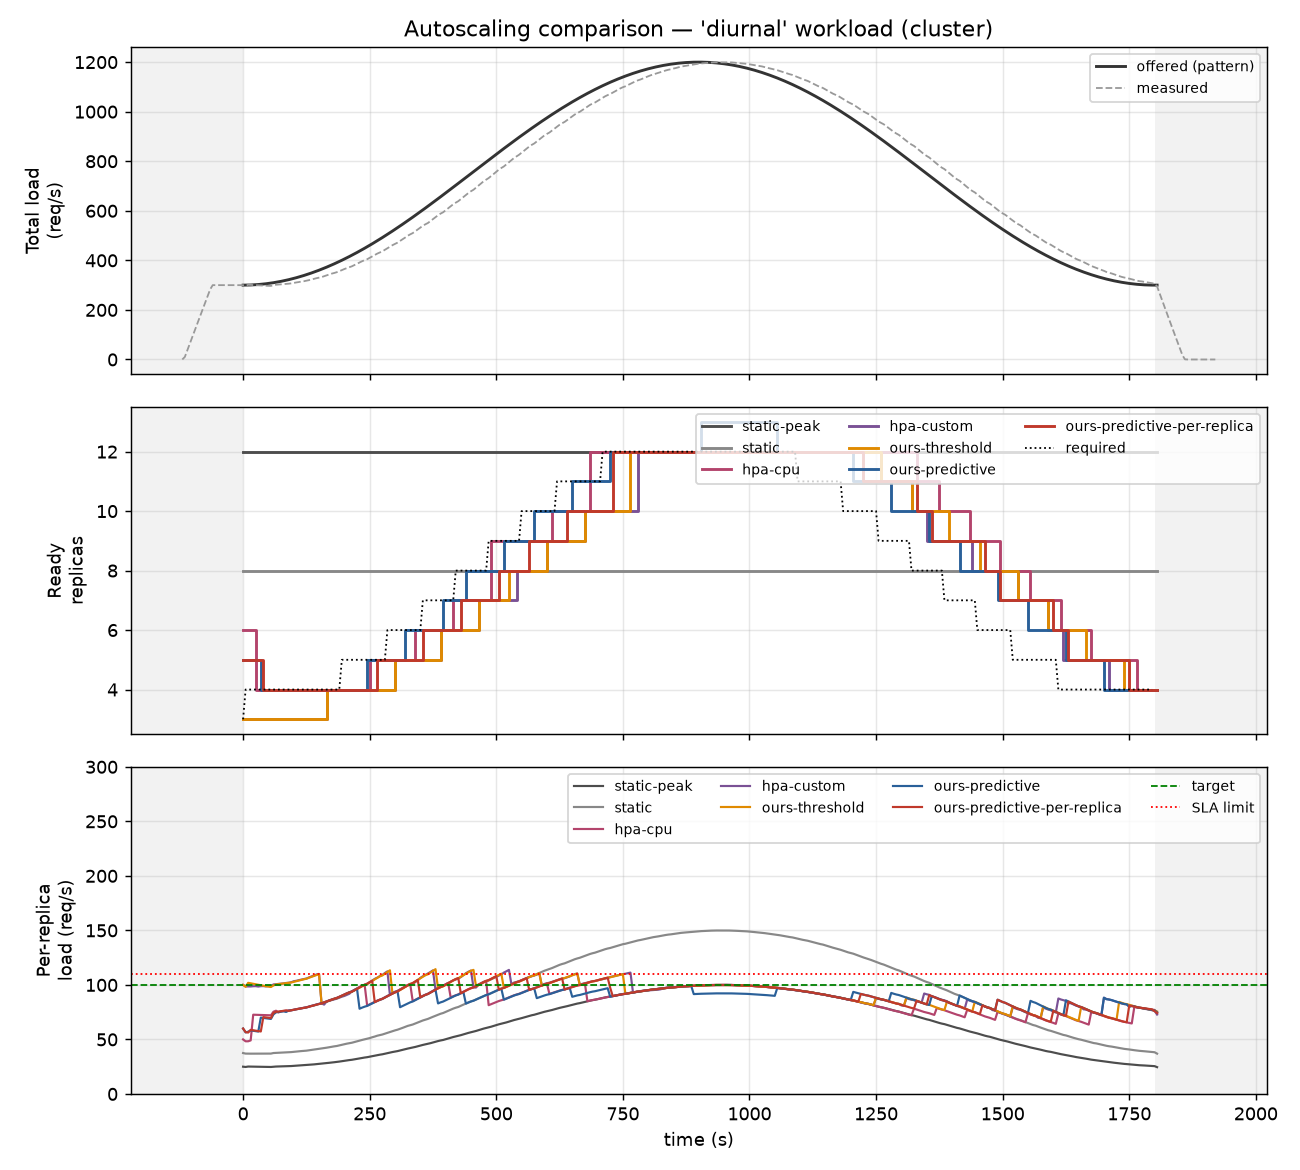
\includegraphics[width=\linewidth]{figures/comparison-diurnal.png}
\caption[مقایسه‌ی بازوها روی بار کاری \lr{diurnal}]{مقایسه‌ی بازوها روی \arm{diurnal}. نوار
خاکستری دو سو، مرحله‌های گرم‌کردن و نشست است و در محاسبه‌ی سنجه‌ها وارد نمی‌شود.}
\label{fig:cmp-diurnal}
\end{figure}

\textbf{\arm{ramp} (شکل~\ref{fig:cmp-ramp}): ستون نقض کیفیت خدمت تفکیک نمی‌کند و این باید
گفته شود.} چهار بازو از شش
بازو روی این الگو ۰/۰ درصد نقض دارند. علتش در خود الگو است: \arm{ramp} در بیست دقیقه ۱۰۰۰
درخواست بر ثانیه بالا می‌رود، یعنی حدود ۰/۸۳ درخواست بر ثانیه در هر ثانیه، یا تقریباً یک
نمونه‌ی اضافی در هر دو دقیقه. این آهنگ آن‌قدر آرام است که یک حلقه‌ی ۱۵ ثانیه‌ای با
راه‌اندازی ۳۰ ثانیه‌ای بتواند به‌صورت واکنشی آن را دنبال کند. ستون‌هایی که در اینجا تفکیک
می‌کنند، \emph{کم‌تأمین منابع} و \emph{زمان واکنش} هستند. گزارش کردن تنها ستون اشباع‌شده،
بازوها را غیرقابل‌تمایز نشان می‌داد در حالی که نیستند.

\begin{figure}[H]
\centering
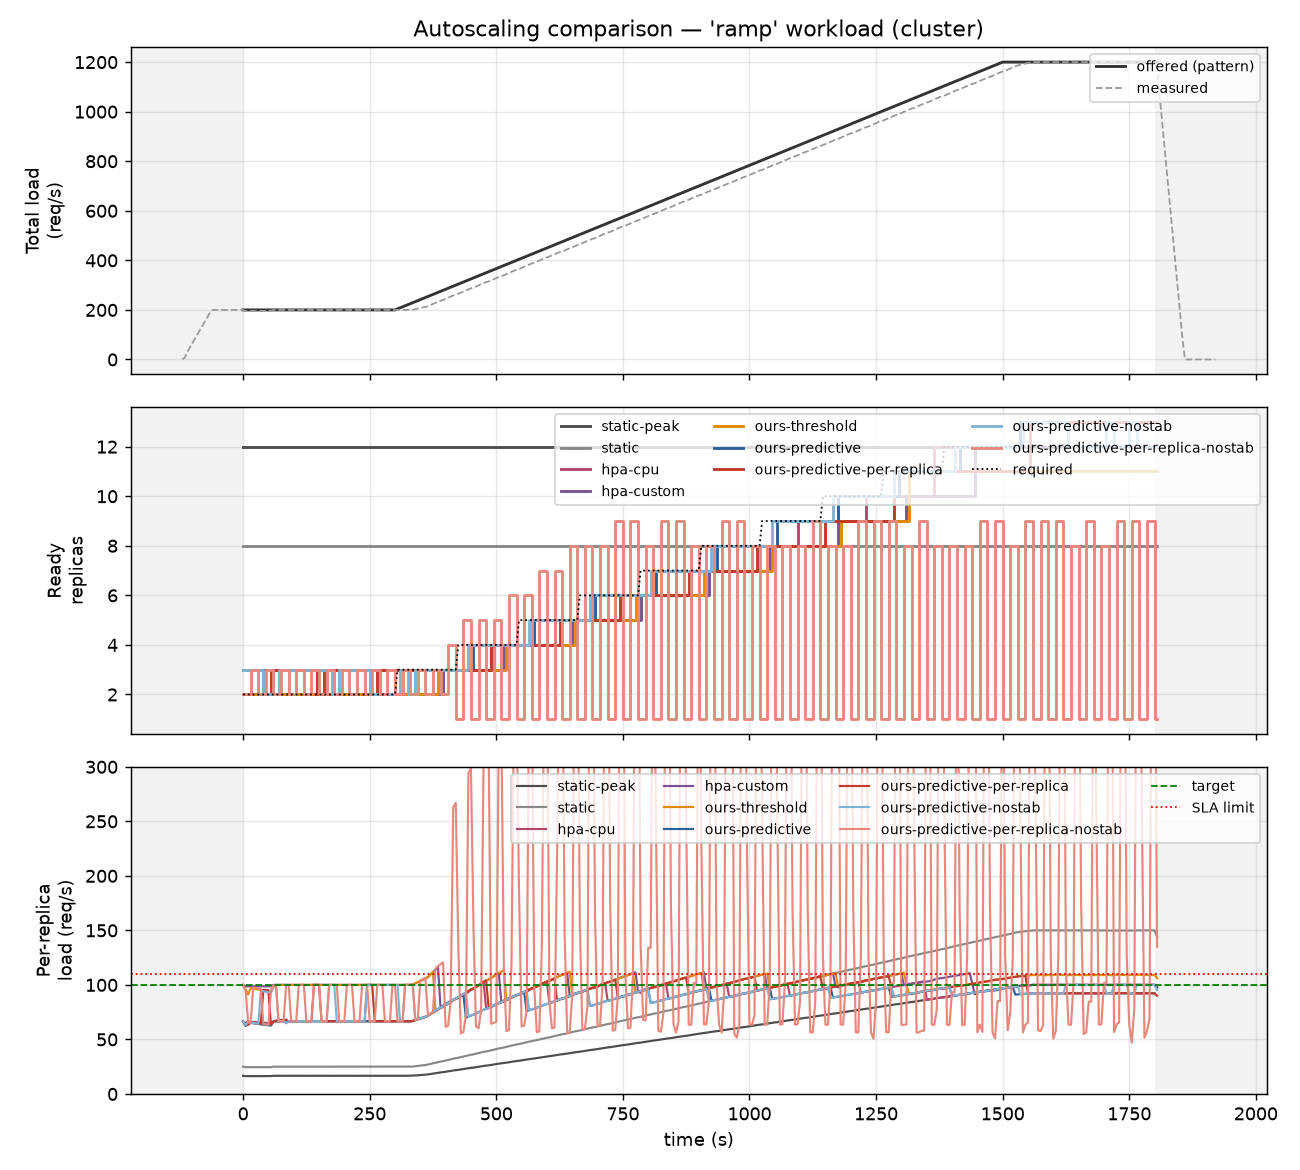
\includegraphics[width=\linewidth]{figures/comparison-ramp.png}
\caption[مقایسه‌ی بازوها روی بار کاری \lr{ramp}]{مقایسه‌ی بازوها روی \arm{ramp}. بازوی
\arm{ours-predictive-per-replica-nostab} ناوگان خود را تا یک نمونه فرو می‌پاشاند.}
\label{fig:cmp-ramp}
\end{figure}

\textbf{\arm{spike} (شکل~\ref{fig:cmp-spike}): نخستین بازوهایی که اصلاً زمان واکنش ندارند.} بازوهای \arm{static} و
\arm{ours-threshold} روی این الگو تا پایان پنجره هرگز به ۱۳ نمونه‌ی لازم نرسیدند. زمان واکنش
برای آن‌ها یک عدد گمشده نیست؛ \emph{خودِ نتیجه} است، و جدول باید آن را چنین بخواند و نه به
شکل خط تیره‌ای که ممکن است «آنی» فهمیده شود.

\begin{figure}[H]
\centering
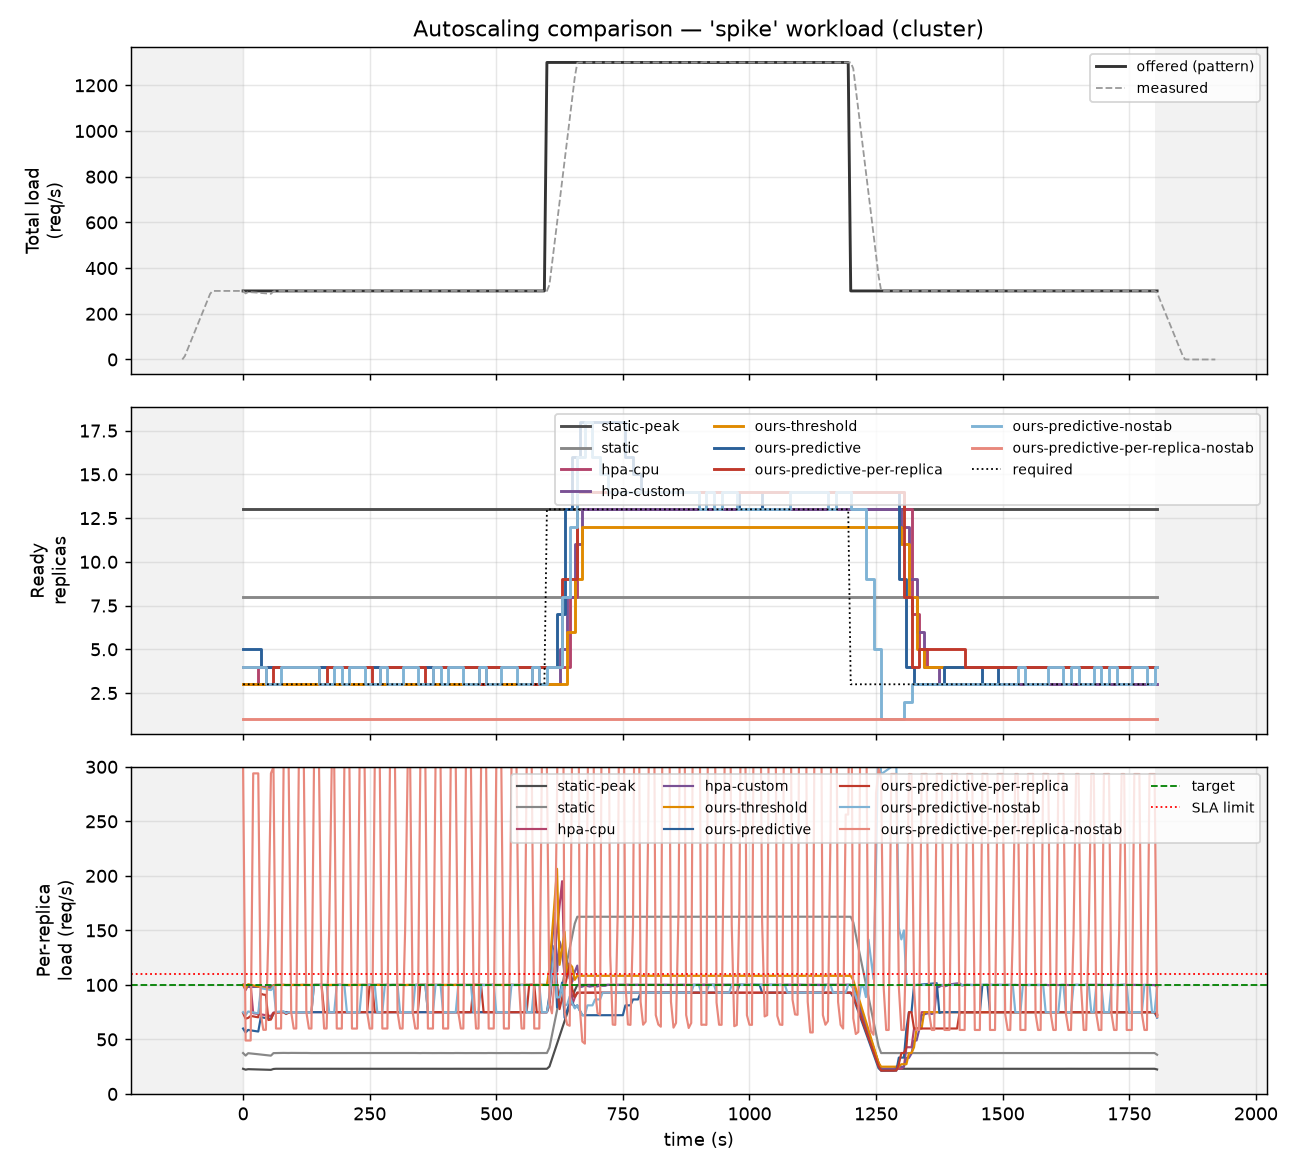
\includegraphics[width=\linewidth]{figures/comparison-spike.png}
\caption[مقایسه‌ی بازوها روی بار کاری \lr{spike}]{مقایسه‌ی بازوها روی \arm{spike}.}
\label{fig:cmp-spike}
\end{figure}

\textbf{\arm{diurnal} (شکل~\ref{fig:cmp-diurnal}): مقایسه‌ی «ارزش مقیاس‌گذاری» در تمیزترین
شکل خود.} روی این الگو
\arm{ours-threshold} با ۱۴،۵۴۵ نمونه-ثانیه در برابر ۱۴،۴۸۰ نمونه-ثانیه‌ی \arm{static} کار
می‌کند \mdash{} یعنی عملاً \emph{همان هزینه} \mdash{} و نقض کیفیت خدمت را از ۴۰/۳ درصد به ۳/۶ درصد
می‌رساند. روشن‌ترین بیان ارزش مقیاس‌گذاری خودکار در این مجموعه همین است.

\begin{figure}[H]
\centering
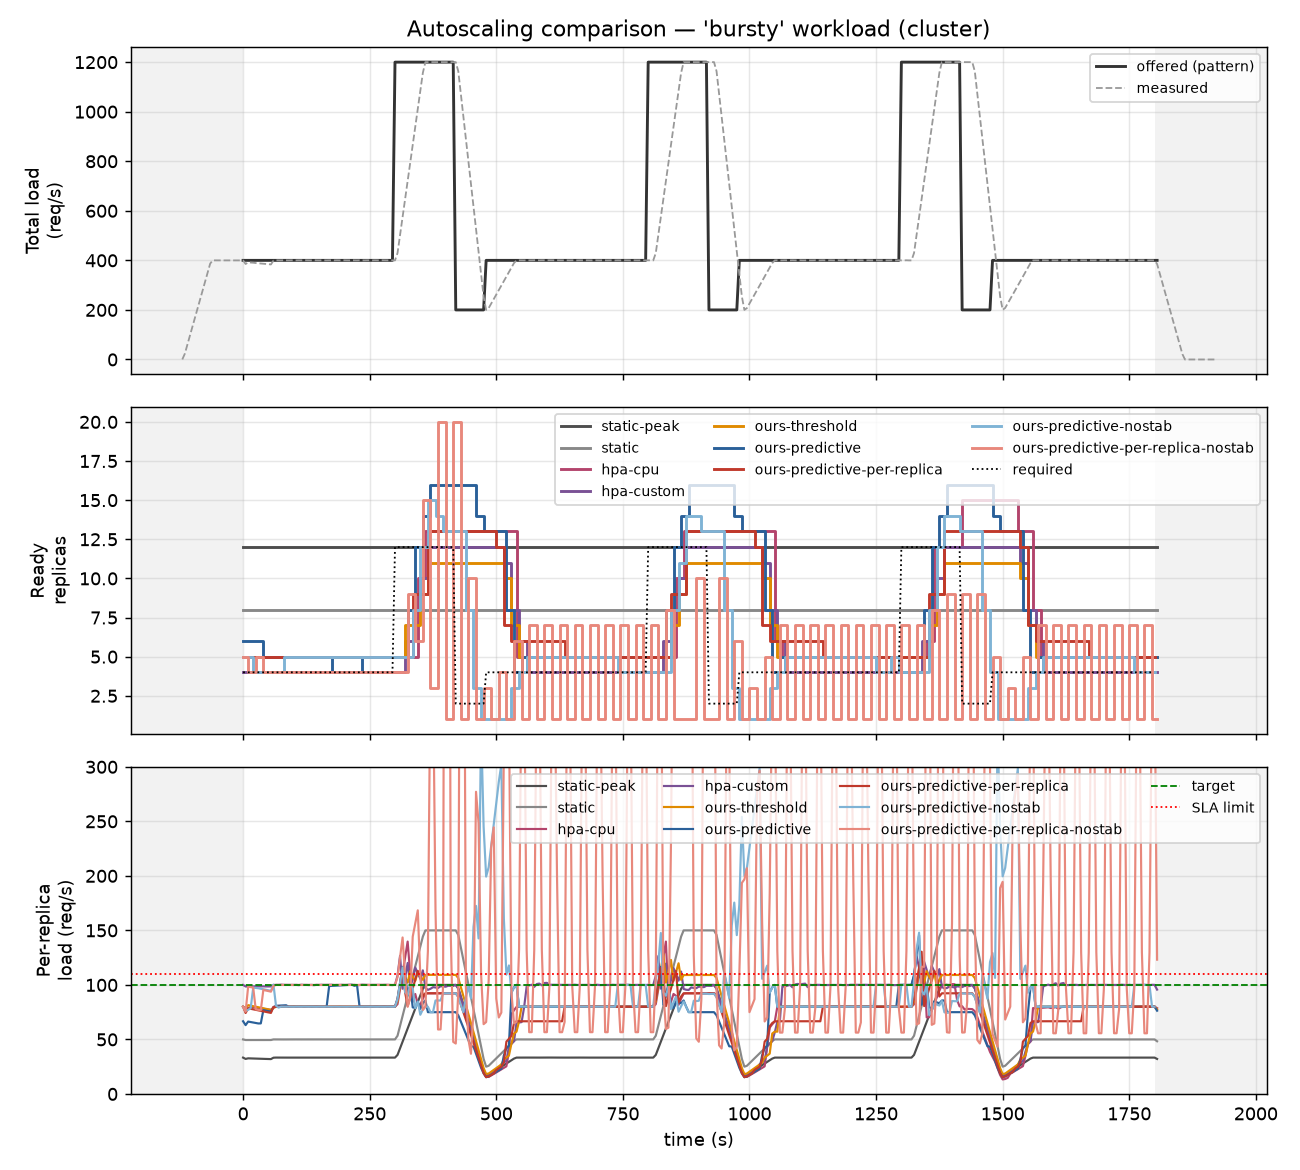
\includegraphics[width=\linewidth]{figures/comparison-bursty.png}
\caption[مقایسه‌ی بازوها روی بار کاری \lr{bursty}]{مقایسه‌ی بازوها روی \arm{bursty}.}
\label{fig:cmp-bursty}
\end{figure}

\textbf{\arm{hpa-cpu} خوب کار می‌کند و باید همین گفته شود.} روی \arm{ramp} و \arm{diurnal}
این بازو ۰/۰ درصد نقض دارد. یک شیب یکنوای آرام، بار کاری‌ای است که \lr{HPA} استاندارد از پس
آن برمی‌آید، و این نوشتار با گفتن آن قوی‌تر است تا با پنهان کردنش.

\subsection{زمان واکنش}
\label{sec:results-reaction}

مقایسه را روی \arm{diurnal} می‌آوریم، چون هر سه کنترل‌گر در آنجا واکنشی سنجیدنی دارند.

\begin{table}[H]
\centering
\caption{زمان واکنش میانه روی \arm{diurnal}}
\label{tab:results-reaction}
\begin{tabular}{|l|r|}
\hline
\textbf{بازو} & \textbf{زمان واکنش (میانه)} \\
\hline
\arm{hpa-custom} & ۱۱۲/۵ ثانیه \\
\arm{ours-threshold} & ۱۰۷/۵ ثانیه \\
\arm{hpa-cpu} & ۵۵/۰ ثانیه \\
\textbf{\arm{ours-predictive}} & \textbf{۲۷/۵ ثانیه} \\
\hline
\end{tabular}
\end{table}

سیاست پیش‌بینانه نزدیک به \textbf{چهار برابر} از \arm{hpa-custom} سریع‌تر است. هر دو دقیقاً
یک سنجه و یک نقطه‌ی هدف دارند. پس این تفاوت را نمی‌توان به کیفیت سنجه نسبت داد و تنها متغیر
باقی‌مانده سیاست است. همین شکل روی هر چهار الگو تکرار می‌شود: زمان واکنش
\arm{ours-predictive} میان ۲۰ تا ۳۵ ثانیه است در برابر ۳۲/۵ تا ۱۲۷/۵ ثانیه برای
\arm{hpa-custom}.

نکته‌ی دومی که ارزش گزارش دارد: \arm{hpa-custom} و \arm{ours-threshold} روی \arm{ramp}
عملاً \emph{بدل یکدیگرند} \mdash{} ۴/۷ در برابر ۴/۱ درصد نقض، ۱۲۷/۵ در برابر ۱۱۰/۰ ثانیه، و ۱۲،۰۴۰
در برابر ۱۱،۸۱۰ نمونه-ثانیه. دو کنترل‌گر واکنشی که مستقل از هم پیاده‌سازی شده‌اند و روی یک
سیگنال کار می‌کنند، در فاصله‌ی ۰/۶ واحد از هم می‌نشینند، که درون قدرت تفکیک اندازه‌گیری است.
این یعنی \textbf{خط مبنای واکنشی ما مثل نمونه‌ی استاندارد رفتار می‌کند}، پس سود پیش‌بینی،
مصنوعِ نوشتن یک رقیب ضعیف نیست.

\subsection{سربار خود مقیاس‌گذار}
\label{sec:results-overhead}

در یک اجرای واقعی، ۱۸ چرخه‌ی آشتی‌دهی مجموعاً ۰/۰۶۸ ثانیه زمان برد، یعنی حدود
\textbf{۳/۸ میلی‌ثانیه بر چرخه} در برابر فاصله‌ی ۱۵ ثانیه‌ای \mdash{} حدود ۰/۰۳ درصد. این عدد
نیازمندی غیرکارکردی «سربار منابع پایین» را برآورده می‌کند و هم‌زمان پرسش «آیا زمان واکنش
اندازه‌گیری‌شده‌ی شما صرفاً کندی کنترل‌گر خودتان نیست؟» را می‌بندد: زمان‌های واکنش
جدول~\ref{tab:results-reaction} از مرتبه‌ی ده‌ها ثانیه‌اند و زمان محاسبه‌ی کنترل‌گر از
مرتبه‌ی میلی‌ثانیه.

\section{آسیب‌شناسی پیش‌بینی بار هر نمونه}
\label{sec:results-perreplica}

یکی از یافته‌های مرکزی این پروژه در پیاده‌سازی به دست آمد و نه در طراحی. سازوکار آن در
بخش~\ref{sec:design-perreplica} توضیح داده شد. این بخش می‌پرسد که آیا آن سازوکار در خوشه‌ی
واقعی دیده می‌شود یا نه \mdash{} و پاسخ، ظریف‌تر از انتظار است.

جدول~\ref{tab:results-reversals} تعداد تغییر جهت را نشان می‌دهد. برای \arm{spike} و
\arm{bursty} سه تکرار مستقل انجام شد و ارقام جداگانه آمده است.

\begin{table}[H]
\centering
\caption{تعداد تغییر جهت؛ بازوی معیوب در برابر بازوی درست}
\label{tab:results-reversals}
\begin{tabular}{|l|l|l|}
\hline
\textbf{بار کاری} & \textbf{\arm{per-replica}} & \textbf{\arm{ours-predictive}} \\
\hline
\arm{ramp} & \lr{5} & \lr{0} \\
\arm{diurnal} & \lr{2} & \lr{2} \\
\arm{spike} & \lr{14, 4, 14} & \lr{3, 5, 7} \\
\arm{bursty} & \lr{10, 6, 5} & \lr{6, 7, 9} \\
\hline
\end{tabular}
\end{table}

نتیجه را باید با احتیاط خواند، و قاعده‌ی بخش~\ref{sec:method-repeatability} همین را ایجاب
می‌کند:

\begin{itemize}
  \item روی \arm{bursty} دو بازو کاملاً هم‌پوشانی دارند و بازوی معیوب حتی اندکی \emph{کمتر}
  نوسان می‌کند. این بار کاری آسیب‌شناسی را نشان نمی‌دهد و ادعای مربوط به آن پس گرفته می‌شود.
  \item روی \arm{spike} جدایی در دو اجرا از سه اجرا دیده می‌شود، اما یک اجرا با عدد ۴ درون
  دامنه‌ی بازوی سالم می‌افتد. شواهد در این شکل \emph{نشانه} است و نه نتیجه‌ی قطعی.
  \item روی \arm{diurnal} هیچ تفکیکی وجود ندارد: ۲ در برابر ۲.
  \item روی \arm{ramp} تفاوت روشن است \mdash{} ۵ در برابر صفر برای \emph{هر} بازوی دیگر.
\end{itemize}

از این تصویر یک نکته‌ی مکانیکی بیرون می‌آید که ارزش آن از خود اعداد بیشتر است. فرض اولیه این
بود که ناپایداری روی بارهایی ظاهر می‌شود که \emph{برمی‌گردند}. این فرض نادرست بود:
\arm{diurnal} برمی‌گردد و نوسان نمی‌کند، و \arm{ramp} هرگز برنمی‌گردد و نوسان می‌کند.

بیان دقیق‌تر آن است که \textbf{تحریک‌کننده‌ی ناپایداری، ناپیوستگی در ورودی یا در مشتق آن
است.} \arm{diurnal} برابر با $300 + 900\sin^2(\pi t / D)$ است و بی‌نهایت بار مشتق‌پذیر \mdash{} و
تنها الگویی است که آسیب‌شناسی در آن ظاهر نمی‌شود. \arm{spike} و \arm{bursty} توابع پله‌ای‌اند،
و \arm{ramp} پیوسته است اما در $t = 300$ و $t = 1500$ ناپیوستگی شیب دارد.

از این نکته یک هشدار عملی به دست می‌آید که مهم‌ترین پیام این بخش است:

\begin{quote}
\textbf{سیاستی که تنها روی یک بار کاری هموار سنجیده شود، پایدار به نظر می‌رسد بی‌آنکه باشد.}
روی \arm{diurnal} بازوی معیوب ۰/۰ درصد نقض دارد و از بازوی درست \emph{ارزان‌تر} هم هست
(۱۴،۹۱۵ در برابر ۱۵،۱۸۰ نمونه-ثانیه). هر کسی که اعتبارسنجی را روی یک منحنی هموار انجام دهد،
این سیاست را عرضه می‌کند.
\end{quote}

با این حال باید صادق بود: شواهد این بخش، به تنهایی، برای اثبات ادعا کافی نیست. اختلاف‌ها در
همان مرتبه‌ی پراکندگی خود بازوها هستند. آنچه ادعا را از این وضعیت ضعیف بیرون می‌آورد، آزمون
حذفی بخش بعد است.

\section{اثر سازوکار پایدارسازی: نتیجه‌ی اصلی}
\label{sec:results-stabilizer}

پرسش پژوهشی دوم این بود: سازوکار پایدارسازی چه مقدار نوسان را پنهان می‌کند و به چه بهایی؟
برای پاسخ، هر دو سیاست پیش‌بینانه یک بار دیگر اجرا شدند، این بار با
\lr{stabilization\_window\_seconds: 0}. یعنی میراگر برداشته شد و \emph{هیچ چیز دیگری} تغییر
نکرد. نتیجه در جدول~\ref{tab:results-nostab} آمده است.

\begin{table}[H]
\centering
\small
\caption{بازوهای حذفی: همان سیاست‌ها با میراگر خاموش}
\label{tab:results-nostab}
\begin{tabular}{|l|l|r|r|r|r|}
\hline
\textbf{بار کاری} & \textbf{بازو} & \textbf{نقض \lr{SLA}} & \textbf{نمونه-ثانیه} & \textbf{بالا/پایین} & \textbf{تغییر جهت} \\
\hline
\arm{spike} & \arm{per-replica-nostab} & \textbf{\lr{50.8\%}} & \lr{1,810} & \lr{60/60} & \textbf{\lr{119}} \\
\arm{spike} & \arm{predictive-nostab} & \lr{4.1\%} & \lr{12,355} & \lr{28/28} & \lr{43} \\
\arm{bursty} & \arm{per-replica-nostab} & \textbf{\lr{42.8\%}} & \lr{7,685} & \lr{49/50} & \textbf{\lr{98}} \\
\arm{bursty} & \arm{predictive-nostab} & \lr{13.0\%} & \lr{10,270} & \lr{27/23} & \lr{21} \\
\arm{ramp} & \arm{per-replica-nostab} & \textbf{\lr{39.5\%}} & \lr{7,360} & \lr{60/60} & \textbf{\lr{119}} \\
\arm{ramp} & \arm{predictive-nostab} & \lr{0.0\%} & \lr{13,395} & \lr{16/7} & \lr{12} \\
\hline
\end{tabular}
\end{table}

یک اجرای ۱۸۰۰ ثانیه‌ای با فاصله‌ی آشتی‌دهی ۱۵ ثانیه، ۱۲۰ چرخه‌ی کنترل دارد.
\textbf{عدد ۶۰ بالا و ۶۰ پایین یعنی کنترل‌گر در هر چرخه‌ی کنترل جهت خود را عوض می‌کند.} این
دیگر نوسان به معنای یک \emph{گرایش} نیست؛ نوسان به نقطه‌ی ثابت سامانه تبدیل شده است.

دو شاهد مستقل این تفسیر را تأیید می‌کنند:

\begin{enumerate}
  \item \textbf{فروپاشی ناوگان.} بازوی معیوب روی \arm{spike} تنها ۱،۸۱۰ نمونه-ثانیه مصرف
  می‌کند در برابر ۱۴،۲۸۰ برای بازوی درست. میانگین نمونه‌های آماده ۱/۰۰ روی \arm{spike}،
  ۴/۰۷ روی \arm{ramp} و ۴/۲۵ روی \arm{bursty} است. رقم \arm{spike} تیزترین بیان این شکست
  است: در سراسر پنجره‌ی ۱۸۰۰ ثانیه‌ای \textbf{شمار نمونه‌های آماده حتی یک بار هم از یک
  بالاتر نرفت}، حال آنکه \code{spec.replicas} تا ۱۱ بالا رفت و در ۱۲۰ حرکت (۶۰ بالا و ۶۰
  پایین) جابه‌جا شد. کنترل‌گر نمونه‌ها را سریع‌تر از آنکه بتوانند آماده شوند درخواست و لغو
  می‌کرد، پس هیچ نمونه‌ی تازه‌ای به خدمت نرسید (۱،۸۱۰ تقسیم بر ۱۸۰۰ برابر ۱/۰۱).
  \item \textbf{کم‌تأمین عظیم.} ۹،۶۲۰ نمونه-ثانیه کم‌تأمین روی \arm{spike}، در برابر ۲۷۰ برای
  بازوی درست.
\end{enumerate}

هر دو شاهد از کمیت‌هایی می‌آیند که مستقل از سری بار هر نمونه‌اند؛ محدودیتی که این سری در
همین سه اجرا دارد در بخش~\ref{sec:validity-metricdiff} ثبت شده است.

حال همین سیاست معیوب را با میراگر ۹۰ ثانیه‌ای بسنجید. روی \arm{ramp} نقض کیفیت خدمت برابر
۰/۰ درصد است و روی \arm{spike} برابر ۰/۶ درصد. یعنی \emph{از همه‌ی آزمون‌های کیفیت و هزینه‌ی
این فصل سربلند بیرون می‌آید}.

نتیجه‌ی اصلی این پایان‌نامه از همین‌جا می‌آید:

\begin{quote}
\textbf{یک پنجره‌ی پایدارسازی ۹۰ ثانیه‌ای می‌تواند یک قانون کنترل بنیاداً معیوب را چنان
بپوشاند که از همه‌ی آزمون‌های کیفیت خدمت و هزینه سربلند بیرون بیاید.}
\end{quote}

این ادعا سه برتری بر شکل اولیه‌ی خود \mdash{} یعنی شمارش تغییر جهت در بخش~\ref{sec:results-perreplica}
\mdash{} دارد. نخست آنکه بزرگی اثر نزدیک به \emph{ده برابر} پراکندگی اندازه‌گیری است و نه درون آن:
۱۱۹ تغییر جهت در برابر ۱۲، و ۵۰/۸ درصد در برابر ۴/۱ درصد. دوم آنکه به شمارش در یک اجرای منفرد
تکیه ندارد و روی هر سه الگوی ناهموار تکرار می‌شود. سوم آنکه \emph{توضیح می‌دهد} چرا سیاست
معیوب روی \arm{diurnal} سالم به نظر می‌رسید: میراگر کار را می‌کرد، و یک بار کاری هموار فشار
چندانی به آن نمی‌آورد.

برای مهندس سامانه نتیجه‌ی عملی روشن است:

\begin{quote}
\textbf{ارزیابی پایداری باید میراگر را خاموش کند و بار کاری پله‌ای بدهد.} وگرنه چیزی را
می‌سنجد که پیشاپیش پنهان شده است.
\end{quote}

توجه شود که این ادعا درباره‌ی \emph{بی‌فایده بودن} میراگر نیست. میراگر کار خودش را به‌خوبی
انجام می‌دهد و بازوی \arm{ours-predictive} نیز به آن نیاز دارد: بدون آن، همان سیاست \emph{درست}
هم روی \arm{bursty} از ۱/۱ به ۱۳/۰ درصد نقض می‌رسد. ادعا این است که میراگر یک
\emph{اصلاح} نیست، و ارزیابی‌ای که آن را روشن نگه دارد نمی‌تواند سالم را از معیوبِ میراشده
تفکیک کند.

\section{مقایسه با شبیه‌ساز}
\label{sec:results-simulator}

برای اعتبارسنجی متقابل، \emph{ترتیب} بازوها در شبیه‌ساز و در خوشه مقایسه شد. مقایسه روی ترتیب
است و نه مقدار مطلق، چون شبیه‌ساز شبکه ندارد و تأخیر راه‌اندازی را ساده مدل می‌کند؛ انتظار
هم‌خوانی مقادیر از ابتدا وجود نداشت.

از هشت ترتیب قابل مقایسه، \textbf{پنج مورد توافق دارند}. هر سه اختلاف روی بارهای کاری
\emph{پله‌ای} رخ داده \mdash{} یعنی \arm{spike} و \arm{bursty} \mdash{} و همگی در یک جهت‌اند: شبیه‌ساز
سیاست واکنشی را جلوتر از سیاست پیش‌بینانه رتبه می‌دهد و خوشه عکس آن را می‌گوید.

علت محتمل روشن است و به بخش~\ref{sec:bg-measurement-lag} برمی‌گردد. شبیه‌ساز بی‌درنگ مقیاس به
پایین می‌دهد و هیچ تأخیر اندازه‌گیری ندارد؛ بار هر نمونه را دقیقاً و بی‌واسطه حساب می‌کند.
خوشه اما پیش از دیدن هر تغییر، یک فاصله‌ی جمع‌آوری به‌علاوه‌ی یک پنجره‌ی یک‌دقیقه‌ای
\lr{rate} هزینه می‌کند. \textbf{تأخیر اندازه‌گیری دقیقاً همان چیزی است که پیش‌بینی جبرانش
می‌کند}، پس حذف آن از مدل، به سود بازوی واکنشی تمام می‌شود.

نتیجه‌ی عملی محدود و مشخص است: شبیه‌ساز برای استدلال درباره‌ی پیکربندی‌ها روی بارهای هموار
قابل اتکاست، اما ترتیب آن روی بارهای پله‌ای قابل اعتماد نیست و هر نتیجه‌ای از آنجا به وارسی
نقطه‌ای روی خوشه نیاز دارد.

\section{تکرارپذیری و قدرت تفکیک}
\label{sec:results-repeatability}

جدول~\ref{tab:results-repeat} نتیجه‌ی تکرارها را نشان می‌دهد. مقادیر به‌جای میانگین‌گیری
تک‌تک آمده‌اند.

\begin{table}[H]
\centering
\small
\caption{اجراهای مستقل تکراری؛ هر مقدار یک اجرای جداگانه است}
\label{tab:results-repeat}
\begin{tabular}{|l|l|l|l|l|}
\hline
\textbf{بار کاری} & \textbf{بازو} & \textbf{نقض \lr{SLA}} & \textbf{نمونه-ثانیه} & \textbf{تغییر جهت} \\
\hline
\arm{spike} & \arm{ours-predictive} & \lr{0.3, 0.8, 0.6} & \lr{14,085 / 14,350 / 14,280} & \lr{3, 5, 7} \\
\arm{spike} & \arm{ours-pred.-per-replica} & \lr{0.8, 0.6, 0.6} & \lr{13,900 / 14,030 / 13,900} & \lr{14, 4, 14} \\
\arm{bursty} & \arm{ours-predictive} & \lr{0.8, 0.3, 1.1} & \lr{14,545 / 14,545 / 14,385} & \lr{6, 7, 9} \\
\arm{bursty} & \arm{ours-pred.-per-replica} & \lr{2.5, 2.2, 1.9} & \lr{13,715 / 13,760 / 13,465} & \lr{10, 6, 5} \\
\arm{ramp} & \arm{ours-threshold} & \lr{5.2, 4.1} & \lr{12,050 / 11,810} & \lr{0, 0} \\
\arm{ramp} & \arm{static} & \lr{35.5, 35.6} & \lr{14,440 / 14,480} & \lr{0, 0} \\
\arm{spike} & \arm{hpa-custom}$^{\dagger}$ & \lr{2.8, 2.8} & \lr{17,105 / 17,055} & \lr{0, 0} \\
\hline
\end{tabular}
\end{table}

\noindent$^{\dagger}$ این دو اجرا \emph{پیش از} اصلاح تحویل بار
(بخش~\ref{sec:results-loaddefect}) انجام شده‌اند و به همین دلیل با سطر \arm{hpa-custom} در
جدول~\ref{tab:results-headline} \mdash{} که از اندازه‌گیری مجدد می‌آید \mdash{} قابل مقایسه نیستند. اینجا
تنها به‌عنوان یک جفت تکرار \emph{هم‌شرایط با یکدیگر} آورده شده‌اند. گروه‌بندی تکرارها بر
پایه‌ی شرایط اجرا و نه صرفاً نام بازو، همان نکته‌ای است که
بخش~\ref{sec:method-repeatability} بر آن تأکید کرد: اگر این دو با اجراهای پس از اصلاح در یک
گروه ریخته می‌شدند، فاصله‌ی میان دو \emph{آزمایش} به‌عنوان نویز \emph{این بازو} گزارش می‌شد و
پراکندگی متورم، یافته‌های واقعی را رد صلاحیت می‌کرد.

سه عدد از این جدول بیرون می‌آید که قدرت تفکیک کل ارزیابی را تعیین می‌کنند:

\begin{itemize}
  \item پراکندگی نمونه-ثانیه برای اجراهای هم‌شرایط میان \textbf{۴۰ تا ۲۹۵} است، یعنی حدود دو
  درصد.
  \item بازوی بدون کنترل‌گر (\arm{static}) تا ۰/۱ درصد بازتولید می‌شود؛ بازوهای خودکار حدود
  یک واحد درصد تغییر می‌کنند. این تفاوت میان اندازه‌گیری یک حلقه‌ی \emph{باز} و یک حلقه‌ی
  \emph{بسته} است.
  \item بنابراین \textbf{تفاوت‌های کمتر از حدود ۱/۵ واحد درصد در نقض کیفیت خدمت میان دو بازوی
  خودکار، در $n=1$ قابل تفکیک نیستند.}
\end{itemize}

بر پایه‌ی همین قاعده بود که در بخش~\ref{sec:results-perreplica} ادعای مربوط به \arm{bursty}
پس گرفته شد و ادعای \arm{spike} به نشانه تنزل یافت. در مقابل، اثر سازوکار پایدارسازی در
بخش~\ref{sec:results-stabilizer} نزدیک به ده برابر این پراکندگی است و به‌راحتی از آن عبور
می‌کند. همین است که آن را به نتیجه‌ی اصلی تبدیل می‌کند و نه یک مشاهده‌ی جالب.

\section{محدودیت‌های اعتبار}
\label{sec:results-validity}

این بخش عمداً مفصل است.

\subsection{تأخیر در این آزمایش تفکیک‌کننده نیست}
\label{sec:results-latency}

«تأخیر پاسخ به کاربر در زمان جهش» یکی از سنجه‌های مقایسه بود. این سنجه در
عمل میان بازوها هیچ تفاوتی نشان نمی‌دهد \mdash{} ستون صدک ۹۵ در هر بازو و هر الگوی بار میان ۲/۴ و ۲/۵
میلی‌ثانیه است \mdash{} و اکنون دلیلش را دقیق می‌دانیم.

محدودیت پردازنده‌ی کانتینر روی این میزبان \emph{اعمال نمی‌شود}. نمونه در بار ۲۲۰۰ درخواست بر
ثانیه ۳/۶۵ هسته مصرف می‌کند حال آنکه \lr{limits.cpu} برابر ۱ است، و شمارنده‌ی دوره‌های
گلوگاه‌شده‌ی زمان‌بند دقیقاً \emph{صفر} می‌ماند. متغیر \lr{GOMAXPROCS} نیز تنظیم نشده، پس
زمان اجرای \lr{Go} هر ۱۴ هسته‌ی گره را می‌بیند. یک نمونه‌ی گرم، ۲۲۰۰ درخواست بر ثانیه را با
صدک ۹۵ برابر ۳/۳۴ میلی‌ثانیه و بدون خطا سرویس می‌دهد.

پس ظرفیت واقعی هر نمونه بیش از ۲۲۰۰ درخواست بر ثانیه است، در برابر نرخ هدف ۱۰۰ \mdash{} یعنی بیش از
بیست برابر. هیچ بازویی در این ارزیابی حتی به یک مرتبه‌ی بزرگی اشباع نزدیک نمی‌شود.

\textbf{عدد ۲/۴ میلی‌ثانیه خطا نیست؛ اندازه‌گیری درستی است که تفکیک نمی‌کند.} تکرار
آزمایش‌ها ستون یکسانی تولید می‌کرد، پس اجرای دوباره برای «به دست آوردن تأخیر واقعی» بی‌فایده
است.

با این حال می‌توان نشان داد که سنجه‌ی تأخیر سالم است و به تأمین منابع پاسخ می‌دهد. تعداد
نمونه تثبیت شد و بار ثابت ۸۰۰ درخواست بر ثانیه داده شد
(جدول~\ref{tab:results-latency-pinned}):

\begin{table}[H]
\centering
\caption{پاسخ تأخیر به تأمین منابع، با ناوگان تثبیت‌شده و بار ثابت ۸۰۰ درخواست بر ثانیه}
\label{tab:results-latency-pinned}
\begin{tabular}{|r|r|r|r|}
\hline
\textbf{نمونه‌ها} & \textbf{تحویل‌شده} & \textbf{تأخیر صدک ۹۵} & \textbf{خطا} \\
\hline
۱ & \lr{792.9} & \textbf{\lr{2276 ms}} & \lr{5.05\%} \\
۲ & \lr{800.6} & \textbf{\lr{2.59 ms}} & \lr{0\%} \\
۴ & \lr{800.0} & \lr{2.60 ms} & \lr{0\%} \\
۸ & \lr{800.0} & \lr{2.65 ms} & \lr{0\%} \\
\hline
\end{tabular}
\end{table}

افزودن \emph{یک} نمونه دُم توزیع تأخیر را نزدیک به ۸۸۰ برابر بهبود می‌دهد. این دو چیز را
نشان می‌دهد: نخست آنکه افزودن نمونه واقعاً ترافیک بیشتری را سرویس می‌دهد \mdash{} که تا پیش از این
آزمایش، هیچ شاهد \emph{فیزیکی} برای آن در داده‌های ارزیابی وجود نداشت \mdash{} و دوم آنکه سنجه‌ی
تأخیر سالم است و فقط در بازه‌ی بار این آزمایش اشباع نشده.

نتیجه‌ی روش‌شناختی روشن است: \textbf{تأخیر در این پایان‌نامه به‌عنوان نتیجه‌ی کالیبراسیون
گزارش می‌شود و نه به‌عنوان سنجه‌ی مقایسه‌ی بازوها.}

\subsection{سنجه‌ی نقض کیفیت خدمت چه چیزی را می‌سنجد}
\label{sec:results-slameaning}

«نقض \lr{SLA}» در این فصل سنجه‌ی \textbf{رزرو ظرفیت} است و نه
سنجه‌ی \textbf{آسیب کاربر}. این سنجه می‌پرسد آیا ناوگان چنان اندازه‌گذاری شده که بار هر نمونه
درون درخواست تضمین‌شده‌ی پردازنده بماند.

این پرسش، پرسش درست و متعارف ظرفیت‌سنجی است، چون ظرفیت مازاد تنها تا وقتی در دسترس است که گره
خلوت باشد و این گره اختصاصی است. اما رقم ۴۰ درصدی نقض به این معنا نیست که کاربران چیزی
دیده‌اند؛ در این آزمایش‌ها ندیده‌اند.

\subsection{نقص تحویل بار}
\label{sec:results-loaddefect}

جدی‌ترین نقص اندازه‌گیری کشف‌شده در این پروژه، و موردی که از تمام بررسی‌های خودکار
بخش~\ref{sec:method-validity} گذشت.

مولد بار به‌صورت پیش‌فرض از اتصال پایدار \lr{HTTP} استفاده می‌کرد. هر کاربر مجازی یک اتصال
\lr{TCP} برای تمام عمرش نگه می‌دارد، و هر اتصال به همان نمونه‌ای سنجاق می‌شود که
\lr{kube-proxy} هنگام باز شدن آن انتخاب کرده است. چون برنامه در حدود ۲/۴ میلی‌ثانیه پاسخ
می‌دهد، سناریوی نرخ‌محور هرگز به بیش از چند کاربر مجازی هم‌زمان نیاز پیدا نکرد \mdash{} و چند کاربر
مجازی یعنی چند اتصال یعنی چند نمونه. جدول~\ref{tab:results-connfix} اثر را مستقیماً نشان
می‌دهد.

\begin{table}[H]
\centering
\caption{آزمون \lr{A/B} کنترل‌شده در ۸۰۰ درخواست بر ثانیه در برابر ۸ نمونه}
\label{tab:results-connfix}
\begin{tabular}{|l|c|r|r|}
\hline
\textbf{مدل اتصال} & \textbf{نمونه‌های سرویس‌دهنده} & \textbf{تحویل‌شده} & \textbf{تأخیر صدک ۹۵} \\
\hline
اتصال پایدار (پیش‌فرض) & \textbf{۱ از ۸} & \lr{508/800} & \textbf{\lr{1.5 s}} \\
اتصال به ازای هر درخواست & \textbf{۷ از ۸} & \lr{800/800} & \lr{2.71 ms} \\
\hline
\end{tabular}
\end{table}

هیچ چیزی در چارچوب این را گزارش نکرد، چون مولد بار نرخ کامل درخواست‌شده را تحویل می‌داد و هر
درخواست هم کد ۲۰۰ برمی‌گرداند.

\textbf{گستره‌ی آسیب اندازه‌گیری شد و به فرض بسنده نشد.} ورودی خود مقیاس‌گذار، چنان‌که در
بخش~\ref{sec:design-collector} آمد، حاصل تقسیم \emph{مجموع} \lr{rate} روی همه‌ی سری‌ها بر
\emph{شمارش} نمونه‌های آماده است و به اینکه کدام نمونه سرویس داده وابسته نیست. هر دو طرف
مستقیماً در میانه‌ی یک اجرا پرس‌وجو شدند: صورت ۱۲۹۹/۹۹ و مخرج ۱۳، یعنی هر دو درست.

اما این استدلال یک حفره دارد: اگر نمونه‌های سنجاق‌شده اشباع می‌شدند، صورت کسر دیگر بار مورد
نظر آزمایش نبود بلکه هر چیزی بود که آن چند نمونه می‌توانستند جذب کنند. پس بار تحویل‌شده در
\emph{تمام ۴۵ اجرای موجود در زمان این بررسی} \mdash{} یعنی ۴۹ اجرای معتبر منهای چهار
اندازه‌گیری مجدد \arm{hpa-custom} که هنوز انجام نشده بود \mdash{} با انتگرال الگو مقابله شد:

\begin{quote}
\textbf{۴۲ اجرا از ۴۵ اجرا در بازه‌ی ۰/۹۹۳ تا ۱/۰۱۰ از مقدار هدف قرار گرفتند.}
\end{quote}

دلیلش ساده است: سه یا چهار نمونه‌ی برنامه‌ای با پاسخ ۲/۴ میلی‌ثانیه‌ای حدود ۱۵۰۰ درخواست بر
ثانیه جذب می‌کنند، که بالاتر از اوج هر الگو در این مجموعه است. بار عرضه‌شده هرگز خفه نشد.

سه استثنا همگی به بازوی \arm{per-replica-nostab} تعلق دارند (نسبت‌های ۰/۳۸۵، ۰/۴۰۹ و ۰/۴۱۳).
این بازو ناوگان خود را فروپاشانده بود، و آنچه کم تحویل شد \emph{خود نتیجه} است و نه نقص
اندازه‌گیری \mdash{} و اگر اثری داشته باشد، ارقام نقض ۳۹ تا ۵۱ درصدی را \emph{محافظه‌کارانه}
می‌کند، چون صورت خفه‌شده مقدار نقض را کم‌برآورد می‌کند.

دو سنجه‌ی متفاوت در کارند و نباید با هم اشتباه شوند: نسبت‌های بالا \emph{سمت ناوگان} را
می‌سنجند (مقدار \code{sum(rate(...))} که واقعاً به برنامه رسید، درون فلات‌های دست‌کم ۱۵۰
ثانیه‌ای)، حال آنکه دروازه‌ی خودکار بخش~\ref{sec:method-validity} شمارش \code{http\_reqs}
خود \lr{k6} را می‌سنجد و روی همین سه اجرا ۰/۹۹۹ و ۰/۹۸۸ و ۰/۹۹۹ گزارش می‌کند. \lr{k6}
تقریباً همه‌ی درخواست‌ها را \emph{فرستاد}؛ ناوگان فروپاشیده تنها بخشی را \emph{سرویس داد}.

ظرفیت یک نمونه هم در دو رژیم اندازه گرفته شده: رقم ۲۲۰۰ درخواست بر ثانیه‌ی
بخش~\ref{sec:results-latency} از یک نمونه‌ی گرم و اختصاصی با مدل اتصال اصلاح‌شده می‌آید،
حال آنکه این سه اجرا پیش از اصلاح و با نمونه‌ای در حال ساخته و نابود شدن انجام شده‌اند
(میانگین بار سرویس‌شده روی \arm{spike} برابر ۳۶۸/۹ درخواست بر ثانیه).

بنابراین نقض کیفیت خدمت، نمونه-ثانیه، کم‌تأمین و بیش‌تأمین، و شمارش تغییر جهت دست‌نخورده
ماندند. آنچه باطل شد دو چیز بود: ستون تأخیر \mdash{} که طبق بخش~\ref{sec:results-latency} به‌هرحال
تفکیک‌کننده نیست \mdash{} و بازوی \arm{hpa-custom} که تنها مصرف‌کننده‌ی سنجه‌ی \emph{هر نمونه} است.
آن بازو روی هر چهار بار کاری از نو اندازه‌گیری شد و همه‌ی ارقام \arm{hpa-custom} در این فصل
از اجرای تازه می‌آید.

دامنه‌ی این اصلاح باید صریح باشد: تنها \textbf{۴ اجرا از ۴۹ اجرای معتبر} زیر قرارداد
اصلاح‌شده گرفته شده‌اند و هر چهار همین اندازه‌گیری‌های \arm{hpa-custom} هستند. ۴۵ اجرای
دیگر \mdash{} از جمله همه‌ی سطرهای جدول~\ref{tab:results-nostab} \mdash{} پیش از اصلاح‌اند و
مجوزشان همان بررسی گستره‌ی آسیب بالاست. میدان \code{load\_contract} در \code{run.json} هر
اجرا این تفکیک را ثبت می‌کند.

\subsection{نتیجه‌ای که با اندازه‌گیری مجدد پس گرفته شد}
\label{sec:results-hpacustom-redo}

اندازه‌گیری مجدد \arm{hpa-custom} یک ادعای پیشین را باطل کرد. صداقت گزارش ایجاب می‌کند که ثبت
شود.

پیش از اصلاح، این بازو روی هیچ بار کاری مقیاس به پایین نمی‌داد و گران‌ترین بازوی خودکار بود.
پس از اصلاح (جدول~\ref{tab:results-hpacustom}):

\begin{table}[H]
\centering
\caption{اثر اصلاح تحویل بار بر بازوی \arm{hpa-custom}}
\label{tab:results-hpacustom}
\begin{tabular}{|l|l|l|r|}
\hline
\textbf{بار کاری} & \textbf{مقیاس به پایین} & \textbf{نمونه-ثانیه} & \textbf{تغییر} \\
\hline
\arm{ramp} & \lr{2 $\rightarrow$ 3} & \lr{12,025 $\rightarrow$ 12,040} & \textbf{‎+۰/۱ درصد} \\
\arm{diurnal} & \lr{1 $\rightarrow$ 11} & \lr{17,115 $\rightarrow$ 14,365} & -۱۶ درصد \\
\arm{spike} & \lr{0--1 $\rightarrow$ 7} & \lr{17,055 $\rightarrow$ 12,255} & -۲۸ درصد \\
\arm{bursty} & \lr{1 $\rightarrow$ 14} & \lr{18,980 $\rightarrow$ 11,965} & -۳۷ درصد \\
\hline
\end{tabular}
\end{table}

سازوکار نیز تأیید شد و صرفاً حدس نماند. قاعده‌ی سنجه‌های غایب \lr{HPA}
(بخش~\ref{sec:bg-hpa}) فرض می‌کند نمونه‌هایی که سنجه ندارند در نقطه‌ی هدف‌اند، و این فرض
\emph{تنها} مسیر مقیاس به پایین را می‌بندد. اگر این سازوکار درست باشد، نقص نباید روی یک بار
کاری \emph{یکنوا} اثری بگذارد. \arm{ramp} تنها بار یکنوای مجموعه است و به اندازه‌ی ۰/۱ درصد
تغییر کرد، در حالی که هر سه بار دیگر به‌شدت جابه‌جا شدند. اثر دقیقاً جایی ظاهر شد که سازوکار
پیش‌بینی می‌کند و جای دیگری ظاهر نشد.

پس ادعای «\lr{HPA} روی سنجه‌ی سفارشی هرگز مقیاس به پایین نمی‌دهد» \textbf{پس گرفته می‌شود}؛
آن رفتار مصنوع مولد بار بود و نه ویژگی سنجه‌های سفارشی.

این اصلاح ادعای خود پروژه را هم جابه‌جا می‌کند. پیش از آن، بازوی
\arm{ours-predictive} روی \arm{diurnal} در هر سه محور هم‌زمان بر \arm{hpa-custom} برتری
داشت. پس از اصلاح، بازوی ما در کیفیت خدمت پیش است (۰/۰ در برابر ۴/۷ درصد) و در زمان واکنش نیز
(۲۷/۵ در برابر ۱۱۲/۵ ثانیه)، اما \textbf{در هزینه ۵/۷ درصد عقب می‌افتد}. همین شکل روی هر
چهار بار کاری تکرار می‌شود.

پس ادعای قابل دفاع همان \emph{مبادله}‌ی بخش~\ref{sec:results-headline} است و نه برتری هم‌زمان
در هر سه محور.

این مورد یک درس روش‌شناختی هم دارد که ارزش آن از خود عدد بیشتر است:
\textbf{یک بازوی مقایسه‌ی معیوب، بازوی خودی را رایگان جلوه می‌دهد.} آزمون حذفی دقیقاً برای
گرفتن همین حالت وجود دارد، و در اینجا تنها به این دلیل کار کرد که آن بازو دوباره اجرا شد و
به آن اعتماد نشد.

\subsection{تفاوت تصویر اجراشده با کد مخزن}
\label{sec:results-image}

اندازه‌گیری‌ها روی تصویری از برنامه‌ی نمونه انجام شد که از روی کد نهایی مخزن ساخته‌شدنی نیست.
بررسی مستقیم نقطه‌ی \lr{/metrics} یک نمونه‌ی در حال اجرا نشان می‌دهد شمارنده‌ی
\code{http\_requests\_shed\_total} در آن وجود ندارد، در حالی که
\code{http\_requests\_in\_flight} هست. پس محتوای آن مقدم بر افزودن سازوکار محدودسازی هم‌زمانی
است. دو پیامد دارد:

\begin{itemize}
  \item \textbf{سنجه‌ی «درخواست‌های ریخته‌شده» در هر ۴۹ اجرا ساختاراً نابینا بوده است.} صفر
  بودنش به معنای رخ‌ندادن نیست، به معنای \emph{نبودن سنجه} است. هر خوانشی از داده‌های این
  پروژه به شکل «هیچ درخواستی ریخته نشد» بی‌پشتوانه است.
  \item \textbf{محدودکننده‌ی ۱۶ درخواست هم‌زمان فعال نبوده است.} در بازوهای
  \arm{per-replica-nostab} شمارش درخواست‌های در جریان روی یک نمونه به ۶۱ رسیده که تنها با
  هم‌زمانی نامحدود ممکن است.
\end{itemize}

در جریان ردیابی این موضوع یک درس عمومی هم به دست آمد:
\textbf{یک برچسب، یک هویت نیست.} انبار تصاویر میزبان و انبار تصاویر گره، دو تصویر
\emph{متفاوت} را زیر یک برچسب یکسان نگه داشته بودند. تنها مرجع قابل اتکا برای اینکه
\lr{kubelet} چه چیزی را اجرا کرده، اثرانگشت ثبت‌شده در وضعیت خود نمونه است.

تصمیم گرفته شد تصویر تثبیت و مستند شود و بازسازی نشود. دلیلش این است که بازسازی، ریختن
درخواست‌ها با کد ۵۰۳ را بالای ۱۶ درخواست هم‌زمان فعال می‌کند و رفتار فیزیکی همه‌ی بازوها را
تغییر می‌دهد \mdash{} به‌ویژه بازوهای فروپاشیده که به ۶۱ رسیده بودند. یعنی آزمایشی \emph{متفاوت}
می‌شود و نه اصلاحی جزئی، و هیچ‌یک از ۴۹ اجرای موجود با آن قابل مقایسه نمی‌ماند. هر ۴۹ اجرا
روی همین یک تصویر انجام شده‌اند، پس نسبت به یکدیگر کاملاً قابل مقایسه‌اند. چارچوب آزمایش اکنون
اثرانگشت را پیش از هر اجرا مقابله می‌کند، اجرایی را که ناوگانش بیش از یک اثرانگشت داشته باشد
رد می‌کند، و اثرانگشت را در فراداده‌ی هر اجرا ثبت می‌کند.

آشتی دادن تصویر و کد مخزن، کاری برای پس از این نوشتار است.

\subsection{هشدار واگرایی سنجه}
\label{sec:validity-metricdiff}

تحلیل‌گر بررسی می‌کند که سری \code{autoscaler\_metric\_value} گزارش‌شده توسط مقیاس‌گذار با
سری \code{per\_replica\_rps} که تحلیل مستقلاً می‌گیرد بخواند، و روی سه اجرای
\arm{per-replica-nostab} اختلاف ۸۶ تا ۱۳۵ درصد گزارش می‌کند. این دو، \emph{یک عبارت
\lr{PromQL} یکسان}‌اند و پس‌خور هر دو را به یک اندازه جابه‌جا می‌کند؛ پس اختلافشان اختلاف
زمان نمونه‌برداری است \mdash{} مقیاس‌گذار روی چرخه‌ی ۱۵ ثانیه‌ای و تحلیل روی شبکه‌ی ۵
ثانیه‌ای، با مخرج \code{count(up)} که میان دو قرائت جابه‌جا می‌شود. معنای این هشدار آن است
که بازسازی تحلیل از سیگنال لزوماً همان چیزی نیست که سیاست بر اساس آن تصمیم گرفته. ارقام
بخش~\ref{sec:results-stabilizer} از آن متأثر نیستند، چون بر شمارش تغییر جهت روی
\code{spec.replicas} و بر نمونه-ثانیه استوارند و هیچ‌کدام از این سری مشتق نمی‌شوند.

\subsection{سایر محدودیت‌ها}
\label{sec:results-otherlimits}

\textbf{تک‌گره و بدون رقابت.} خوشه یک گره اختصاصی ۱۴ هسته‌ای است. ظرفیت مازادی که در
بخش~\ref{sec:results-latency} دیده شد، روی گره‌ای که با سرویس‌های دیگر مشترک باشد در دسترس
نخواهد بود. نتایج به خوشه‌های چندمستأجری تعمیم‌پذیر نیستند بدون اندازه‌گیری دوباره.

\textbf{تعداد تکرار.} تنها چند بازو سه بار تکرار شده‌اند. نتایجی که به تفاوت‌های کوچک وابسته
بودند در این فصل به‌عنوان نشانه گزارش شده‌اند و نه نتیجه.

\textbf{یک سرویس، بدون‌حالت.} هیچ زنجیره‌ی چندسرویسی آزموده نشده است. در چنین زنجیره‌ای،
مقیاس‌گیری یک سرویس بار سرویس بعدی را تغییر می‌دهد و مسیر پس‌خور تازه‌ای می‌سازد که این
ارزیابی آن را نمی‌بیند.

\textbf{اثر رگبار سرد.} نخستین رگبار بار روی یک نمونه‌ی سرد تأخیر صدک ۹۵ حدود ۲/۵ ثانیه و ۱۳
تا ۲۶ درصد خطا نشان می‌دهد، در حالی که همان نمونه در حالت گرم چنین رفتاری ندارد. این حالت پس
از حدود سه دقیقه بی‌کاری بازمی‌گردد، پس گذرای مقیاس به پایین نیست. سازوکارش هنوز روشن نیست.
هر اجرای اندازه‌گیری‌شده با مرحله‌ی گرم‌کردن آغاز می‌شود، پس نتایج این فصل از آن متأثر
نیستند. با این حال این پدیده ممکن است سود پیش‌بینی را از راهی توضیح دهد که سنجه‌های فعلی
نمی‌بینند \mdash{} نمونه‌ای که \emph{پیش از} رسیدن بار افزوده شود گرم است، و نمونه‌ای که واکنشی
افزوده شود سرد \mdash{} و برای کار آینده پیشنهاد می‌شود.

\section{جمع‌بندی فصل}
\label{sec:results-summary}

\textbf{درباره‌ی کارایی.} در میان بازوهای خودکار، سیاست پیش‌بینانه روی هر چهار بار کاری
کم‌ترین کم‌تأمین منابع را دارد و نقض کیفیت خدمتش کم‌ترین یا هم‌تراز کم‌ترین است، و زمان
واکنشش روی \arm{diurnal} نزدیک به چهار برابر بهتر از
\arm{hpa-custom} است که همان سیگنال و همان نقطه‌ی هدف را دارد. اما این برتری به بهای ۵/۷ تا ۲۰/۲
درصد ظرفیت بیشتر به دست می‌آید. \textbf{ادعای درست یک مبادله است و نه برتری مطلق.}

\textbf{درباره‌ی پایداری.} پیش‌بینی بار هر نمونه به‌جای بار کل، حلقه‌ی کنترل را ناپایدار
می‌کند. با میراگر روشن، این ناپایداری در سنجه‌های متعارف تقریباً دیده نمی‌شود و روی یک بار
کاری هموار اصلاً دیده نمی‌شود.

\textbf{نتیجه‌ی اصلی.} با خاموش کردن میراگر، همان سیاست تا ۵۰/۸ درصد نقض کیفیت خدمت و ۱۱۹
تغییر جهت در ۱۲۰ چرخه‌ی کنترل می‌رسد. پس یک پنجره‌ی پایدارسازی ۹۰ ثانیه‌ای می‌تواند یک قانون
کنترل معیوب را چنان بپوشاند که از همه‌ی آزمون‌ها سربلند بیرون بیاید. \textbf{ارزیابی پایداری
باید میراگر را خاموش کند و بار کاری پله‌ای بدهد.}

\textbf{درباره‌ی اعتبار.} تأخیر در بازه‌ی بار این آزمایش تفکیک‌کننده نیست و به‌عنوان نتیجه‌ی
کالیبراسیون گزارش شده است. سنجه‌ی نقض کیفیت خدمت سنجه‌ی رزرو ظرفیت است و نه سنجه‌ی آسیب
کاربر. یک نقص تحویل بار کشف و اندازه‌گیری شد و بازوی آسیب‌دیده از نو اجرا شد، که به پس گرفتن
یکی از قوی‌ترین ادعاهای پیشین انجامید. و تصویر اندازه‌گیری‌شده از کد مخزن ساخته‌شدنی نیست،
که ثبت شده و تثبیت شده است.

\chapter{جمع‌بندی و کارهای آینده}
\label{ch:conclusion}

\section{خلاصه‌ی کار انجام‌شده}
\label{sec:conclusion-summary}

در این پروژه یک مقیاس‌گذار خودکار افقی به زبان \lr{Go} طراحی و پیاده‌سازی شد که سیگنال
مقیاس‌گذاری را با یک عبارت \lr{PromQL} پیکربندی‌پذیر از \lr{Prometheus} می‌خواند، اندازه‌ی
ناوگان را با یکی از سه سیاست تصمیم می‌گیرد، و آن را از راه زیرمنبع \lr{scale} روی
\lr{Kubernetes} اعمال می‌کند. معماری در امتداد سه دغدغه‌ی مستقل شکسته شد و هر مرحله واسطی با
دست‌کم دو پیاده‌سازی دارد.

سپس این مقیاس‌گذار روی یک خوشه‌ی واقعی و در برابر چهار الگوی بار و نُه بازوی مقایسه ارزیابی
شد. ارزیابی شامل ۴۹ اجرای معتبر با مقیاس زمانی حقیقی است که هر کدام ۱۸۰۰ ثانیه اندازه‌گیری
دارند، به‌علاوه‌ی یک چارچوب آزمایش با بررسی اعتبار خودکار که اجراهای معیوب را پیش از ورود به
تحلیل کنار می‌گذارد.

اما همان‌گونه که در بخش~\ref{sec:intro-question} گفته شد، خود مقیاس‌گذار \emph{ابزار} این
پژوهش است و نه دستاورد آن. دستاورد، پاسخ‌هایی است که در ادامه می‌آید.

\section{پاسخ به پرسش‌های پژوهش}
\label{sec:conclusion-answers}

\subsection*{پرسش ۱: کدام سیگنال حلقه را ناپایدار می‌کند؟}

پاسخ ساختاری است و نه صرفاً تجربی. پیش‌بینی باید روی سیگنالی انجام شود که
\textbf{برون‌زا} باشد؛ یعنی سیگنالی که کنش‌های خود کنترل‌گر آن را جابه‌جا نکند.

بار هر نمونه، $m(t) = \lambda(t)/r(t)$، درون‌زاست چون $r(t)$ خروجی خود کنترل‌گر است.
برون‌یابی آن یک مسیر بسته با بهره‌ی مثبت می‌سازد: مقیاس به بالا باعث افت بار هر نمونه
می‌شود، پیش‌بینی‌کننده این افت را ادامه‌دار می‌بیند، مقیاس به پایین توصیه می‌کند، و چرخه از
نو آغاز می‌شود.

نرخ کل ورود درخواست‌ها، $\lambda(t)$، برون‌زاست چون مقیاس‌گذار نمی‌تواند تعداد درخواست‌های
کاربران را تغییر دهد. سازمایه‌ی این تفاوت را می‌توان مستقیماً در فرمول دید: در
$d = \lceil \hat{\lambda}/T \rceil$ هیچ وابستگی‌ای به $r$ وجود ندارد، پس بهره‌ی آن مسیر
\emph{ساختاراً} صفر است.

این پاسخ در سه سطح مستقل تأیید شد: در آزمون واحد حلقه‌بسته (۲۹ تغییر در برابر صفر، زیر بار کل
ثابت)، در شبیه‌ساز (۱۷ تغییر در برابر ۳، با ۲۳ درصد هزینه‌ی بیشتر و بدون سود)، و در خوشه‌ی
واقعی (بخش~\ref{sec:results-stabilizer}).

مشاهده‌ی تکمیلی و غیرمنتظره‌ی این پروژه آن است که تحریک‌کننده‌ی ناپایداری، \emph{ناپیوستگی در
ورودی یا در مشتق آن} است و نه صرفاً برگشتن بار. تنها الگوی هموارِ مجموعه، تنها الگویی است که
آسیب‌شناسی در آن ظاهر نمی‌شود.

\subsection*{پرسش ۲: میراگر چه مقدار را می‌پوشاند؟}

تقریباً همه‌اش را، و این نتیجه‌ی اصلی این پایان‌نامه است.

با پنجره‌ی پایدارسازی ۹۰ ثانیه‌ای، سیاست معیوب روی \arm{ramp} صفر درصد و روی \arm{spike} ۰/۶
درصد نقض کیفیت خدمت دارد و روی \arm{diurnal} حتی از سیاست درست \emph{ارزان‌تر} است. با
خاموش کردن همان میراگر و بدون هیچ تغییر دیگری، همان سیاست به ۳۹ تا ۵۱ درصد نقض و ۹۸ تا ۱۱۹
تغییر جهت در ۱۲۰ چرخه‌ی کنترل می‌رسد و ناوگان خود را تا یک نمونه فرو می‌پاشاند.

\begin{quote}
\textbf{یک پنجره‌ی پایدارسازی ۹۰ ثانیه‌ای می‌تواند یک قانون کنترل بنیاداً معیوب را چنان
بپوشاند که از همه‌ی آزمون‌های کیفیت خدمت و هزینه سربلند بیرون بیاید.}
\end{quote}

بهایی که این پوشاندن دارد در سنجه‌های متعارف پیدا نیست، و همین است که آن را خطرناک می‌کند.
پیامد عملی برای هر کسی که یک سیاست مقیاس‌گذاری را ارزیابی می‌کند این است: \textbf{ارزیابی
پایداری باید میراگر را خاموش کند و بار کاری با ناپیوستگی بدهد.}

\subsection*{پرسش ۳: پیش‌بینی چه می‌خرد، و بهایش چیست؟}

پاسخ یک \textbf{مبادله} است و نه یک برتری.

پیش‌بینی، کیفیت خدمت و سرعت واکنش می‌خرد: در میان بازوهای خودکار، کم‌ترین کم‌تأمین منابع
روی هر چهار بار کاری و کم‌ترین یا هم‌تراز کم‌ترین نقض، و زمان واکنش ۲۰ تا ۳۵ ثانیه در برابر
۳۲/۵ تا ۱۲۷/۵ ثانیه برای \arm{hpa-custom} که همان سیگنال و همان نقطه‌ی هدف را دارد. بهای
آن، ۵/۷ تا ۲۰/۲ درصد ظرفیت بیشتر است.

این پاسخ در جریان کار یک بار \emph{قوی‌تر} بیان شده بود و پس گرفته شد. آن بیان قوی‌تر بر
داده‌ای استوار بود که یک نقص در مولد بار تولید کرده بود؛ اندازه‌گیری مجدد بازوی مقایسه نشان
داد که برتری در محور هزینه وجود ندارد (بخش~\ref{sec:results-hpacustom-redo}).

پرسش سوم یک بخش دیگر هم داشت: سود پیش‌بینی روی کدام جنس بار کاری وجود دارد؟ پاسخ، یک
\textbf{نتیجه‌ی منفی نسبت به پیشنهاد اولیه‌ی پروژه} است. پیشنهاد مدعی بود پیش‌بینی به
«جهش‌های ناگهانی ترافیک» کمک می‌کند. این ادعا نادرست است و اندازه‌گیری خلافش را نشان می‌دهد:
هیچ پیش‌بینی‌کننده‌ای یک پله‌ی آنی را از پیش نمی‌بیند، و روی \arm{spike} سیاست پیش‌بینانه در
همان لحظه‌ای واکنش نشان می‌دهد که سیاست آستانه‌ای.

ادعای قابل دفاع این است: \textbf{پیش‌بینی روی بارهای روندار و دوره‌ای کمک می‌کند و روی
پله‌های پیش‌بینی‌ناپذیر ذاتاً نمی‌تواند کمک کند.} این بیان ضعیف‌تر از ادعای پیشنهاد است و
دقیقاً به همین دلیل قابل دفاع است.

\section{درس‌های مهندسی}
\label{sec:conclusion-lessons}

جدا از پاسخ‌های بالا، چند درس عملی در جریان کار به دست آمد که ارزش ثبت مستقل دارند. وجه
مشترک همه‌ی آن‌ها این است که به‌جای شکست پرسروصدا، نتایج را \emph{بی‌سروصدا} خراب می‌کنند.

\textbf{یک مقیاس‌گذار مبتنی بر سنجه‌های برنامه، دقیقاً وقتی نابینا می‌شود که بیش از همه به آن
نیاز است.} زیر بار اضافی، محدودیت پردازنده کانتینر را منجمد می‌کند، نقطه‌ی سنجه‌ها پاسخ
نمی‌دهد، پرس‌وجو بردار تهی برمی‌گرداند، و مقیاس‌گذار آن را \mdash{} به‌درستی \mdash{} صفر می‌خواند
(بخش~\ref{sec:method-observability-collapse}). هیچ مؤلفه‌ای اشتباه نمی‌کند و مجموع شکست
می‌خورد.

\textbf{چارچوب آزمایش خودش یک دستگاه اندازه‌گیری است.} سه نقص در کد \emph{بررسی‌کننده} پیدا
شد و نه در سامانه‌ی تحت آزمون، و هر سه در جهت رد کردن اجراهای \emph{سالم} سوگیری داشتند
(بخش~\ref{sec:method-instrument}). دستگاهی که هرگز روی ورودی معلوم خوانده نشده، کالیبره نشده
است.

\textbf{یک گیت که به دلیل اشتباه شلیک می‌کند، از نبودِ گیت فقط اندکی بهتر است}، چون نفر بعدی
را به سراغ اشکال‌زدایی مؤلفه‌ی درست نمی‌فرستد.

\textbf{یک برچسب، یک هویت نیست} (بخش~\ref{sec:results-image}). تنها مرجع قابل اتکا برای اینکه
چه چیزی اجرا شده، اثرانگشت ثبت‌شده در وضعیت خود نمونه است.

\textbf{یک بازوی مقایسه‌ی معیوب، بازوی خودی را رایگان جلوه می‌دهد}
(بخش~\ref{sec:results-hpacustom-redo}). این دقیقاً همان حالتی است که آزمون حذفی برای گرفتن آن
وجود دارد، و تنها به این دلیل گرفته شد که آن بازو دوباره اجرا شد و به آن اعتماد نشد.

\textbf{نوشتن آزمون به‌مثابه‌ی مشخصه، نقص‌هایی را آشکار می‌کند که خواندن کد آشکار نمی‌کند}
(بخش~\ref{sec:design-defects}). هر سه نقص مسیر کنترل تنها در بدترین وضعیت خوشه فعال می‌شدند.

\section{محدودیت‌ها}
\label{sec:conclusion-limitations}

محدودیت‌های اعتبار به‌تفصیل در بخش~\ref{sec:results-validity} آمده‌اند و در اینجا فقط فهرست
می‌شوند تا خواننده بتواند دامنه‌ی تعمیم نتایج را بسنجد:

\begin{itemize}
  \item خوشه تک‌گره و بدون رقابت با مستأجران دیگر است.
  \item تأخیر در بازه‌ی بار این آزمایش تفکیک‌کننده نیست؛ ظرفیت واقعی هر نمونه بیش از بیست
  برابر نرخ هدف است.
  \item سنجه‌ی نقض کیفیت خدمت، رزرو ظرفیت را می‌سنجد و نه آسیب مشاهده‌شده‌ی کاربر.
  \item تنها چند بازو سه بار تکرار شده‌اند؛ قدرت تفکیک حدود ۱/۵ واحد درصد است.
  \item تنها یک سرویس بدون‌حالت آزموده شده و هیچ زنجیره‌ی چندسرویسی در کار نیست.
  \item تصویر اندازه‌گیری‌شده از کد نهایی مخزن ساخته‌شدنی نیست؛ تثبیت و مستند شده است.
\end{itemize}

\section{کارهای آینده}
\label{sec:conclusion-future}

\textbf{اشتقاق تحلیلی مرز پایداری.} در این نوشتار، شرط پایداری به‌صورت \emph{ساختاری} بیان شد
(برون‌زا در برابر درون‌زا) و به‌صورت تجربی تأیید شد. گام بعدی، به دست آوردن یک شرط کمّی بر
حسب افق پیش‌بینی $h$، ضریب هموارسازی $\alpha$، فاصله‌ی آشتی‌دهی و تأخیر راه‌اندازی است، و
سپس اعتبارسنجی مرز پیش‌بینی‌شده در برابر یک جاروب پارامتری در شبیه‌ساز. با توجه به آنچه
بخش~\ref{sec:results-simulator} درباره‌ی محدودیت شبیه‌ساز روی بارهای پله‌ای گفت، هر نتیجه‌ی
چنین جاروبی به وارسی نقطه‌ای روی خوشه نیاز دارد.

\textbf{جاروب سود پیش‌بینی در برابر تأخیر راه‌اندازی.} تمام استدلال این پروژه بر نسبت میان
«سرعت حرکت بار» و «زمان آماده‌شدن نمونه» استوار است. تغییر دادن سیستماتیک عامل دوم \mdash{} که با
تزریق تأخیر مصنوعی در کاوشگر آمادگی ساده است \mdash{} یک یافته‌ی تعمیم‌پذیر می‌دهد: از چه تأخیری به
بعد پیش‌بینی می‌ارزد.

\textbf{مدل هزینه و قاعده‌ی تصمیم سربه‌سر.} با توجه به اینکه نتیجه یک مبادله است، پرسش عملی
بعدی این است که با چه نسبتی میان هزینه‌ی ظرفیت و هزینه‌ی نقض کیفیت خدمت، سیاست پیش‌بینانه
انتخاب درستی است. داده‌های موجود برای ساختن چنین مدلی کافی است.

\textbf{افزودن \lr{KEDA} به‌عنوان بازوی پنجم.} این کار مقایسه را به رایج‌ترین ابزار عملی
بوم‌سازگان گسترش می‌دهد.

\textbf{پیش‌بینی‌کننده‌های سنگین‌تر.} \lr{ARIMA} یا \lr{LSTM} پشت همان واسط
\code{Forecaster}. باید تأکید کرد که این کار تنها با رعایت یافته‌ی این پروژه معنا دارد: هر
پیش‌بینی‌کننده‌ی جدید باید نرخ ورود \emph{برون‌زا} را پیش‌بینی کند و نه سیگنالی را که
کنترل‌گر جابه‌جا می‌کند. پیش‌بینی‌کننده‌ی دقیق‌تر روی سیگنال نادرست، تنها ناپایداری را
سریع‌تر می‌کند.

\textbf{اثر رگبار سرد.} پدیده‌ای که در بخش~\ref{sec:results-otherlimits} گزارش شد،
بازتولیدپذیر است اما سازوکارش ناشناخته است. اگر تأیید شود، مسیری است که از راه آن پیش‌بینی
می‌تواند سودی بدهد که سنجه‌های فعلی این پروژه اصلاً نمی‌بینند: نمونه‌ای که پیش از رسیدن بار
افزوده شود گرم است و نمونه‌ای که واکنشی افزوده شود سرد.

\textbf{زنجیره‌های چندسرویسی.} در یک زنجیره، مقیاس‌گیری یک سرویس بار سرویس بعدی را تغییر
می‌دهد. این یک مسیر پس‌خور تازه است، و با توجه به یافته‌ی مرکزی این پروژه، دقیقاً همان جنس
ساختاری است که ارزش بررسی دارد.

\textbf{آشتی دادن تصویر و کد مخزن}، مطابق آنچه در بخش~\ref{sec:results-image} توضیح داده شد.

\section{سخن پایانی}
\label{sec:conclusion-final}

این پروژه با هدف ساختن یک مقیاس‌گذار خودکار سفارشی آغاز شد و با یافته‌ای درباره‌ی
\emph{ارزیابی} مقیاس‌گذارها پایان یافت. تغییر مسیر از یک اندازه‌گیری در هفته‌ی نخست آمد که
نشان داد نمونه‌ی اولیه سیگنال نادرستی را پیش‌بینی می‌کند \mdash{} و مهم‌تر از آن، نشان داد که این
خطا در سنجه‌های متعارف تقریباً نامرئی است.

آنچه در نهایت به‌عنوان مهم‌ترین نتیجه ثبت شد، درباره‌ی هیچ‌یک از سیاست‌ها نیست، بلکه درباره‌ی
روشی است که با آن سیاست‌ها سنجیده می‌شوند: سازوکاری که برای بهبود رفتار سامانه ساخته شده
است \mdash{} و کارش را هم به‌خوبی انجام می‌دهد \mdash{} می‌تواند هم‌زمان توانایی ما در دیدن یک نقص بنیادی را
از بین ببرد. یک ارزیابی که تنها پیکربندی نهایی را می‌سنجد، نمی‌تواند بگوید نتیجه‌ی خوب از
درستی قانون کنترل آمده است یا از میراگری که رویش گذاشته شده.


%--------------------------------------------------------- مراجع و پیوست‌ها
\chapterfont{\vspace*{-2em}\centering\LARGE}%

\appendix
\bibliographystyle{plain-fa}
\bibliography{references}
\chapter*{پیوست‌ها}
\markboth{پیوست‌ها}{}
\addcontentsline{toc}{chapter}{پیوست‌ها}

این بخش سه پیوست دارد. پیوست الف پیکربندی کاملی را می‌آورد که همه‌ی اندازه‌گیری‌ها با آن
انجام شده‌اند. پیوست ب راهنمای بازتولید آزمایش‌هاست. پیوست ج جدول‌های کامل نتایج را به تفکیک
هر الگوی بار در بر می‌گیرد.

%=============================================================================
\section*{پیوست الف \mdash{} پیکربندی}
\addcontentsline{toc}{section}{پیوست الف \mdash{} پیکربندی}
%=============================================================================

\subsection*{الف-۱: پیکربندی مقیاس‌گذار}

این فایل در خوشه به شکل \lr{ConfigMap} نصب می‌شود. طرح آن عمداً با فایل پیکربندی شبیه‌ساز
یکی است تا مقایسه‌ی فصل~\ref{ch:results} با تفاوت تنظیمات مخدوش نشود.

\begin{latin}
\begin{lstlisting}[language=yamlx]
interval_seconds: 15

collector:
  type: prometheus
  url: http://prometheus-operated.monitoring.svc:9090
  timeout_seconds: 5
  # Requests per second per *ready* replica.
  query: >
    sum(rate(http_requests_total{app="sample"}[1m]))
      / clamp_min(count(up{app="sample"} == 1), 1)

policy:
  name: predictive       # threshold | predictive | predictive-per-replica
  target: 100.0          # requests/second/replica
  tolerance: 0.10        # HPA's 10% dead-band
  min_replicas: 1
  max_replicas: 20
  forecaster:
    type: ewma           # ewma | holt
    horizon: 3           # steps ahead; 3 x 15s = 45s of lead time
    alpha: 0.5
  stabilization_window_seconds: 90
  cooldown_seconds: 0    # disabled in every measured run
  max_step: 0            # disabled in every measured run

scaler:
  type: kubernetes
  deployment: sample
  namespace: default

exporter:
  enabled: true
  port: 8000
\end{lstlisting}
\end{latin}

در بازوهای حذفی، تنها یک مقدار تغییر می‌کند: \lr{stabilization\_window\_seconds: 0}.

\subsection*{الف-۲: بازوی \lr{hpa-cpu}}

نکته‌ی کلیدی، مقدار \lr{averageUtilization: 100} است و نه مقدار متعارف ۷۰. دلیل آن در
بخش~\ref{sec:method-calibration} توضیح داده شد: تنها با این مقدار، این بازو و بازوی
\arm{ours-threshold} به یک نقطه‌کار نشانه می‌روند. بلوک \lr{behavior} نیز عمداً آینه‌ی
سازوکار پایدارسازی خود ماست تا مقایسه، \emph{سیگنال} و \emph{سیاست} را جدا کند و نه
تفاوت‌های اتفاقی در میراسازی را.

\begin{latin}
\begin{lstlisting}[language=yamlx]
apiVersion: autoscaling/v2
kind: HorizontalPodAutoscaler
metadata:
  name: sample-hpa-cpu
spec:
  scaleTargetRef:
    apiVersion: apps/v1
    kind: Deployment
    name: sample
  minReplicas: 1
  maxReplicas: 20
  metrics:
    - type: Resource
      resource:
        name: cpu
        target:
          type: Utilization
          averageUtilization: 100
  behavior:
    scaleUp:
      stabilizationWindowSeconds: 0
      policies:
        - {type: Percent, value: 100, periodSeconds: 15}
    scaleDown:
      stabilizationWindowSeconds: 90
      policies:
        - {type: Percent, value: 100, periodSeconds: 15}
\end{lstlisting}
\end{latin}

\subsection*{الف-۳: بازوی \lr{hpa-custom} و قاعده‌ی \lr{Prometheus Adapter}}

این بازو همان سنجه و همان نقطه‌ی هدف سیاست ما را دارد و تنها متغیر باقی‌مانده، سیاست است.

\begin{latin}
\begin{lstlisting}[language=yamlx]
# HorizontalPodAutoscaler
  metrics:
    - type: Pods
      pods:
        metric:
          name: http_requests_per_second
        target:
          type: AverageValue
          averageValue: "100"

# prometheus-adapter rule
rules:
- seriesQuery: 'http_requests_total{namespace!="",pod!=""}'
  resources:
    overrides:
      namespace: {resource: "namespace"}
      pod: {resource: "pod"}
  name:
    matches: "^http_requests_total$"
    as: "http_requests_per_second"
  metricsQuery: 'sum(rate(<<.Series>>{<<.LabelMatchers>>}[1m])) by (<<.GroupBy>>)'
\end{lstlisting}
\end{latin}

پنجره‌ی \lr{[1m]} در \lr{metricsQuery} عمداً با پنجره‌ی \lr{PromQL} خود مقیاس‌گذار یکی است.

\subsection*{الف-۴: منابع برنامه‌ی نمونه}

سه مقدار در این مانیفست بار معنایی دارند و در فصل‌های پیشین به هر سه ارجاع داده شده است.

\begin{latin}
\begin{lstlisting}[language=yamlx]
env:
  - {name: WORK_CPU_MS,         value: "2"}    # calibration: 100 rps x 2ms = 200m
  - {name: WORK_MAX_CONCURRENT, value: "16"}   # not active in the measured image
resources:
  requests: {cpu: 200m,  memory: 32Mi}         # the HPA utilisation denominator
  limits:   {cpu: 1000m, memory: 64Mi}         # raised from 400m; see 4-3-1

readinessProbe:                                # decides when a replica "counts"
  httpGet: {path: /healthz, port: http}
  initialDelaySeconds: 1
  periodSeconds: 2
  timeoutSeconds: 3
  failureThreshold: 3

livenessProbe:                                 # must detect a *deadlocked* process
  httpGet: {path: /healthz, port: http}
  initialDelaySeconds: 10
  periodSeconds: 15
  timeoutSeconds: 5
  failureThreshold: 6
\end{lstlisting}
\end{latin}

سرویس هدف از نوع \lr{LoadBalancer} تعریف شده است و نه \lr{ClusterIP}، به دلیلی که در
بخش~\ref{sec:design-sampleapp} آمد.

%=============================================================================
\section*{پیوست ب \mdash{} راهنمای بازتولید آزمایش‌ها}
\addcontentsline{toc}{section}{پیوست ب \mdash{} راهنمای بازتولید}
%=============================================================================

\subsection*{ب-۱: پیش‌نیازها}

\lr{Go 1.26}، \lr{Docker}، \lr{kubectl}، \lr{Helm}، \lr{k6}، و \lr{Python 3.11} یا بالاتر
برای برنامه‌ی تحلیل. یک خوشه‌ی \lr{Kubernetes} محلی لازم است؛ پیکربندی سه‌گره‌ی \lr{kind} در
مخزن موجود است.

\subsection*{ب-۲: برپاسازی}

\begin{latin}
\begin{lstlisting}
make stack-up      # monitoring + dashboards + sample app + ServiceMonitors + autoscaler
make load          # drive one workload by hand
make experiment    # one measured run of one arm
make sweep         # every arm on one pattern (~3 hours)
make analyze       # derive every metric from the stored captures
\end{lstlisting}
\end{latin}

\subsection*{ب-۳: نکاتی که بدون دانستنشان بازتولید شکست می‌خورد}

\textbf{مقیاس زمانی باید یک باشد.} چارچوب، اجرای با مقیاس زمانی متفاوت را بدون پرچم صریح
«دودی» رد می‌کند. دلیل آن در بخش~\ref{sec:method-timescale} آمده است. یک بازو حدود ۳۴ دقیقه و
یک جاروب کامل حدود سه ساعت طول می‌کشد.

\textbf{میزبان نباید بخوابد.} دستور متعارف جلوگیری از خواب تنها خوابِ بی‌کاری را متوقف
می‌کند. تنها راه قابل اتکا در این آزمایش‌ها، باز نگه داشتن درِ دستگاه برای تمام مدت بود
(بخش~\ref{sec:method-unattended}). خواب میزبان برای بازوهای پیش‌بینانه \emph{بازیابی‌ناپذیر}
است: یک شکاف در ورودی، تاریخچه‌ی پیش‌بینی‌کننده را خراب می‌کند و آنچه پس از بیداری دیده
می‌شود، سیاست در حال بازیابی از یک قطعی ورودی است و نه سیاست تحت آزمون.

\textbf{اجرای بدون سرپرست نباید فرزند نشستی باشد که آن را تماشا می‌کند.}

\textbf{کشیدن تصاویر از برخی مخازن ممکن است شکست بخورد.} روی میزبان این پروژه، کشیدن تصویر از
\lr{quay.io} و \lr{ghcr.io} توسط \lr{kubelet} با خطای ۵۰۰ شکست می‌خورد در حالی که
\lr{registry.k8s.io} بی‌مشکل کار می‌کند. راه‌حل، کشیدن دستی تصویر روی میزبان پیش از نصب چارت
است. این مشکل مربوط به شبکه‌ی محلی است و کسی که پشت یک اتصال معمولی باشد آن را نخواهد دید؛ اما
کسی که پشت همان واسط باشد بلافاصله به آن برمی‌خورد.

\textbf{تصویر برنامه‌ی نمونه با اثرانگشت تثبیت شده است.} چارچوب پیش از هر اجرا آن را مقابله
می‌کند و در صورت اختلاف، پیش از عرضه‌ی هر باری متوقف می‌شود. دلیل این تصمیم در
بخش~\ref{sec:results-image} آمده است.

\subsection*{ب-۴: آنچه هر اجرا به‌جا می‌گذارد}

هر اجرا یک پوشه با فراداده‌ی اجرا، ۱۷ سری زمانی خام، خلاصه‌ی مولد بار و گزارش کامل آن تولید
می‌کند. فراداده شامل نام بازو، الگو، پنجره‌ی زمانی، وضعیت اعتبار و دلایل نامعتبری، اثرانگشت
تصویر، و شیوه‌ی تحویل بار است. \textbf{هیچ سنجه‌ای در حین اجرا محاسبه نمی‌شود.} همه‌ی
سنجه‌ها بعداً از روی همین سری‌های خام مشتق می‌شوند، و به همین دلیل هر تعریف نادرست را می‌توان
اصلاح و همه‌ی اجراهای گذشته را بدون بازگشت به خوشه دوباره امتیازدهی کرد.

%=============================================================================
\section*{پیوست ج \mdash{} جدول‌های کامل نتایج}
\addcontentsline{toc}{section}{پیوست ج \mdash{} جدول‌های کامل نتایج}
%=============================================================================

جدول‌های~\ref{tab:app-spike} تا~\ref{tab:app-ramp} تنها پنجره‌ی اندازه‌گیری را در بر
می‌گیرند؛ مرحله‌های گرم‌کردن و نشست
کنار گذاشته شده‌اند. «نیاز» برابر $\lceil \lambda(t)/100 \rceil$ از تعریف الگوست و نه از بار
تحویل‌شده. علامت «\lr{---}» در ستون زمان واکنش یعنی ناوگان تا پایان پنجره هرگز به عدد لازم نرسید؛
این یک عدد گمشده نیست، بلکه خود نتیجه است.

\begin{table}[H]
\centering
\scriptsize
\caption{نتایج کامل \mdash{} \arm{spike}}
\label{tab:app-spike}
\setlength{\tabcolsep}{3pt}
\begin{tabular}{|l|r|r|r|r|r|r|r|r|}
\hline
\textbf{بازو} & \textbf{\lr{SLA}} & \textbf{نمونه-ث} & \textbf{کم‌تأمین} & \textbf{بیش‌تأمین} & \textbf{هسته-ث} & \textbf{واکنش} & \textbf{بالا/پایین} & \textbf{جهت} \\
\hline
\arm{static-peak} & \lr{0.0\%} & \lr{23,530} & \lr{0} & \lr{12,100} & \lr{2,464.3} & \lr{---} & \lr{0/0} & \lr{0} \\
\arm{static} & \lr{32.9\%} & \lr{14,480} & \lr{3,000} & \lr{6,050} & \lr{2,449.5} & \lr{---} & \lr{0/0} & \lr{0} \\
\arm{hpa-cpu} & \lr{1.7\%} & \lr{13,915} & \lr{480} & \lr{2,965} & \lr{2,409.9} & \lr{60.0} & \lr{3/4} & \lr{1} \\
\arm{hpa-custom} & \lr{2.2\%} & \lr{12,255} & \lr{475} & \lr{1,300} & \lr{2,506.2} & \lr{70.0} & \lr{4/5} & \lr{1} \\
\arm{ours-threshold} & \lr{2.5\%} & \lr{11,925} & \lr{1,095} & \lr{1,590} & \lr{2,404.5} & \lr{---} & \lr{3/4} & \lr{1} \\
\arm{ours-predictive} & \lr{0.6\%} & \lr{14,280} & \lr{270} & \lr{3,120} & \lr{2,440.2} & \lr{35.0} & \lr{7/9} & \lr{7} \\
\arm{ours-pred.-per-replica} & \lr{0.6\%} & \lr{13,900} & \lr{390} & \lr{2,860} & \lr{2,419.9} & \lr{60.0} & \lr{9/9} & \lr{14} \\
\arm{ours-pred.-nostab} & \lr{4.1\%} & \lr{12,355} & \lr{465} & \lr{1,390} & \lr{2,365.3} & \lr{60.0} & \lr{28/28} & \lr{43} \\
\arm{ours-pred.-per-rep.-nostab} & \lr{50.8\%} & \lr{1,810} & \lr{9,620} & \lr{0} & \lr{1,356.9} & \lr{---} & \lr{60/60} & \lr{119} \\
\hline
\end{tabular}
\end{table}

\noindent\textbf{یادداشت‌های \arm{spike}:} بازوهای \arm{static}، \arm{ours-threshold} و
\arm{ours-pred.-per-replica-nostab} پس از پله‌ی $t=600$ هرگز به ۱۳ نمونه‌ی آماده نرسیدند. در
بازوی آخر، سنجه‌ی داخلی مقیاس‌گذار ۱۳۵ درصد (میانه) از بار مشاهده‌شده‌ی هر نمونه واگرا شد.

\begin{table}[H]
\centering
\scriptsize
\caption{نتایج کامل \mdash{} \arm{diurnal}}
\label{tab:app-diurnal}
\setlength{\tabcolsep}{3pt}
\begin{tabular}{|l|r|r|r|r|r|r|r|r|}
\hline
\textbf{بازو} & \textbf{\lr{SLA}} & \textbf{نمونه-ث} & \textbf{کم‌تأمین} & \textbf{بیش‌تأمین} & \textbf{هسته-ث} & \textbf{واکنش} & \textbf{بالا/پایین} & \textbf{جهت} \\
\hline
\arm{static-peak} & \lr{0.0\%} & \lr{21,720} & \lr{0} & \lr{7,290} & \lr{2,907.8} & \lr{---} & \lr{0/0} & \lr{0} \\
\arm{static} & \lr{40.3\%} & \lr{14,480} & \lr{2,490} & \lr{2,540} & \lr{2,895.9} & \lr{---} & \lr{0/0} & \lr{0} \\
\arm{hpa-cpu} & \lr{0.0\%} & \lr{15,570} & \lr{370} & \lr{1,510} & \lr{2,894.1} & \lr{55.0} & \lr{6/9} & \lr{2} \\
\arm{hpa-custom} & \lr{4.7\%} & \lr{14,365} & \lr{1,070} & \lr{1,005} & \lr{2,998.5} & \lr{112.5} & \lr{8/8} & \lr{1} \\
\arm{ours-threshold} & \lr{3.6\%} & \lr{14,545} & \lr{1,025} & \lr{1,140} & \lr{2,854.7} & \lr{107.5} & \lr{8/8} & \lr{1} \\
\arm{ours-predictive} & \lr{0.0\%} & \lr{15,180} & \lr{245} & \lr{995} & \lr{2,880.6} & \lr{27.5} & \lr{9/10} & \lr{2} \\
\arm{ours-pred.-per-replica} & \lr{0.0\%} & \lr{14,915} & \lr{600} & \lr{1,085} & \lr{2,874.9} & \lr{72.5} & \lr{7/9} & \lr{2} \\
\hline
\end{tabular}
\end{table}

\noindent\textbf{یادداشت‌های \arm{diurnal}:} بازوی \arm{static} پس از چهار پله‌ی متوالی هرگز
به ۹، ۱۰، ۱۱ و ۱۲ نمونه‌ی لازم نرسید. بازوهای حذفی روی این الگو اجرا نشدند.

\begin{table}[H]
\centering
\scriptsize
\caption{نتایج کامل \mdash{} \arm{bursty}}
\label{tab:app-bursty}
\setlength{\tabcolsep}{3pt}
\begin{tabular}{|l|r|r|r|r|r|r|r|r|}
\hline
\textbf{بازو} & \textbf{\lr{SLA}} & \textbf{نمونه-ث} & \textbf{کم‌تأمین} & \textbf{بیش‌تأمین} & \textbf{هسته-ث} & \textbf{واکنش} & \textbf{بالا/پایین} & \textbf{جهت} \\
\hline
\arm{static-peak} & \lr{0.0\%} & \lr{21,720} & \lr{0} & \lr{11,960} & \lr{2,094.8} & \lr{---} & \lr{0/0} & \lr{0} \\
\arm{static} & \lr{17.4\%} & \lr{14,480} & \lr{1,440} & \lr{6,160} & \lr{2,091.7} & \lr{---} & \lr{0/0} & \lr{0} \\
\arm{hpa-cpu} & \lr{2.5\%} & \lr{13,880} & \lr{1,200} & \lr{5,320} & \lr{2,085.5} & \lr{30.0} & \lr{7/6} & \lr{5} \\
\arm{hpa-custom} & \lr{4.4\%} & \lr{11,965} & \lr{1,260} & \lr{3,465} & \lr{2,087.3} & \lr{32.5} & \lr{12/12} & \lr{5} \\
\arm{ours-threshold} & \lr{3.3\%} & \lr{12,365} & \lr{1,410} & \lr{4,015} & \lr{2,088.1} & \lr{0.0} & \lr{9/9} & \lr{5} \\
\arm{ours-predictive} & \lr{1.1\%} & \lr{14,385} & \lr{960} & \lr{5,585} & \lr{2,070.4} & \lr{20.0} & \lr{16/15} & \lr{9} \\
\arm{ours-pred.-per-replica} & \lr{1.9\%} & \lr{13,465} & \lr{1,215} & \lr{4,940} & \lr{2,077.2} & \lr{32.5} & \lr{6/12} & \lr{5} \\
\arm{ours-pred.-nostab} & \lr{13.0\%} & \lr{10,270} & \lr{1,805} & \lr{2,335} & \lr{2,026.6} & \lr{67.5} & \lr{27/23} & \lr{21} \\
\arm{ours-pred.-per-rep.-nostab} & \lr{42.8\%} & \lr{7,685} & \lr{4,145} & \lr{2,070} & \lr{1,635.4} & \lr{12.5} & \lr{49/50} & \lr{98} \\
\hline
\end{tabular}
\end{table}

\noindent\textbf{یادداشت‌های \arm{bursty}:} بازوهای \arm{static} و \arm{ours-threshold} پس از
هر سه رگبار هرگز به ۱۲ نمونه نرسیدند. در بازوی \arm{ours-pred.-per-rep.-nostab} سنجه‌ی داخلی
مقیاس‌گذار ۸۶ درصد (میانه) واگرا شد.

\begin{table}[H]
\centering
\scriptsize
\caption{نتایج کامل \mdash{} \arm{ramp}}
\label{tab:app-ramp}
\setlength{\tabcolsep}{3pt}
\begin{tabular}{|l|r|r|r|r|r|r|r|r|}
\hline
\textbf{بازو} & \textbf{\lr{SLA}} & \textbf{نمونه-ث} & \textbf{کم‌تأمین} & \textbf{بیش‌تأمین} & \textbf{هسته-ث} & \textbf{واکنش} & \textbf{بالا/پایین} & \textbf{جهت} \\
\hline
\arm{static-peak} & \lr{0.0\%} & \lr{21,720} & \lr{0} & \lr{8,450} & \lr{2,640.8} & \lr{---} & \lr{0/0} & \lr{0} \\
\arm{static} & \lr{35.6\%} & \lr{14,480} & \lr{2,420} & \lr{3,630} & \lr{2,631.2} & \lr{---} & \lr{0/0} & \lr{0} \\
\arm{hpa-cpu} & \lr{0.0\%} & \lr{12,990} & \lr{605} & \lr{325} & \lr{2,586.0} & \lr{70.0} & \lr{8/0} & \lr{0} \\
\arm{hpa-custom} & \lr{4.7\%} & \lr{12,040} & \lr{1,230} & \lr{0} & \lr{2,671.8} & \lr{127.5} & \lr{9/0} & \lr{0} \\
\arm{ours-threshold} & \lr{4.1\%} & \lr{11,810} & \lr{1,460} & \lr{0} & \lr{2,476.7} & \lr{110.0} & \lr{8/0} & \lr{0} \\
\arm{ours-predictive} & \lr{0.0\%} & \lr{13,515} & \lr{270} & \lr{575} & \lr{2,585.1} & \lr{30.0} & \lr{10/0} & \lr{0} \\
\arm{ours-pred.-per-replica} & \lr{0.0\%} & \lr{12,900} & \lr{885} & \lr{515} & \lr{2,475.9} & \lr{87.5} & \lr{11/3} & \lr{5} \\
\arm{ours-pred.-nostab} & \lr{0.0\%} & \lr{13,395} & \lr{200} & \lr{325} & \lr{2,482.3} & \lr{20.0} & \lr{16/7} & \lr{12} \\
\arm{ours-pred.-per-rep.-nostab} & \lr{39.5\%} & \lr{7,360} & \lr{6,540} & \lr{630} & \lr{1,496.6} & \lr{10.0} & \lr{60/60} & \lr{119} \\
\hline
\end{tabular}
\end{table}

\noindent\textbf{یادداشت‌های \arm{ramp}:} بازوهای \arm{static}، \arm{ours-threshold} و
\arm{ours-pred.-per-rep.-nostab} در پله‌های پایانی هرگز به ۱۲ نمونه نرسیدند. در بازوی آخر،
سنجه‌ی داخلی مقیاس‌گذار ۸۸ درصد (میانه) واگرا شد.

\subsection*{ج-۵: توزیع اجراها}

جدول~\ref{tab:app-runcount} شمار اجراهای گزارش‌شده را به تفکیک دسته می‌آورد.

\begin{table}[H]
\centering
\caption{شمار اجراهای گزارش‌شده در این نوشتار}
\label{tab:app-runcount}
\begin{tabular}{|l|r|}
\hline
\textbf{دسته} & \textbf{شمار} \\
\hline
اجراهای معتبر با مقیاس زمانی حقیقی & \lr{49} \\
\quad از این میان: چهار الگو × هفت بازوی اصلی & \lr{28} \\
\quad بازوهای حذفی (سه الگو × دو بازو) & \lr{6} \\
\quad تکرارها و اندازه‌گیری‌های مجدد & \lr{15} \\
\hline
اجراهای دودی (مقیاس زمانی $\neq$ ۱) & گزارش نشده \\
اجراهای نامعتبر & کنار گذاشته‌شده، با ثبت دلیل \\
\hline
\end{tabular}
\end{table}


%------------------------------------------------------------------ واژه‌نامه‌ها
\parindent=0pt
%
\chapter*{واژه‌نامه‌ی فارسی به انگلیسی}
\pagestyle{style9}

\addcontentsline{toc}{chapter}{واژه‌نامه‌ی فارسی به انگلیسی}
%%%%%%
\begin{multicols*}{2}

{\bf آ - ا}
\vspace*{3mm}

\farsiTOenglish{آشتی‌دهنده}{Reconciler}
\farsiTOenglish{اثرانگشت تصویر}{Image Digest}
\farsiTOenglish{ارکستراسیون کانتینر}{Container Orchestration}

\vspace*{3mm}
{\bf ب}
\vspace*{3mm}

\farsiTOenglish{بار کاری}{Workload}
\farsiTOenglish{برون‌زا}{Exogenous}
\farsiTOenglish{برون‌یابی}{Extrapolation}
\farsiTOenglish{بهره‌ی حلقه}{Loop Gain}
\farsiTOenglish{بیش‌تأمین منابع}{Over-provisioning}

\vspace*{3mm}
{\bf پ}
\vspace*{3mm}

\farsiTOenglish{پس‌خور}{Feedback}
\farsiTOenglish{پنجره‌ی پایدارسازی}{Stabilization Window}
\farsiTOenglish{پیش‌بینانه}{Predictive / Proactive}
\farsiTOenglish{پیش‌بینی‌کننده}{Forecaster}

\vspace*{3mm}
{\bf ت}
\vspace*{3mm}

\farsiTOenglish{تفکیک دغدغه‌ها}{Separation of Concerns}
\farsiTOenglish{تغییر جهت}{Direction Reversal}
\farsiTOenglish{توافق سطح خدمت}{Service Level Agreement}

\vspace*{3mm}
{\bf ج - ح}
\vspace*{3mm}

\farsiTOenglish{جمع‌آورنده‌ی سنجه}{Metric Collector}
\farsiTOenglish{حلقه‌ی بسته}{Closed Loop}

\vspace*{3mm}
{\bf د - ر}
\vspace*{3mm}

\farsiTOenglish{درون‌زا}{Endogenous}
\farsiTOenglish{رایانش ابری}{Cloud Computing}
\farsiTOenglish{ریزخدمت}{Microservice}

\vspace*{3mm}
{\bf س}
\vspace*{3mm}

\farsiTOenglish{سنجه‌ی سطح‌برنامه}{Application-level Metric}
\farsiTOenglish{سیاست آستانه‌ای}{Threshold Policy}

\vspace*{3mm}
{\bf ط - ک}
\vspace*{3mm}

\farsiTOenglish{طول صف}{Queue Length}
\farsiTOenglish{کاوشگر آمادگی}{Readiness Probe}
\farsiTOenglish{کاوشگر زنده‌بودن}{Liveness Probe}
\farsiTOenglish{کشسانی}{Elasticity}
\farsiTOenglish{کم‌تأمین منابع}{Under-provisioning}

\vspace*{3mm}
{\bf م}
\vspace*{3mm}

\farsiTOenglish{مقیاس‌گذاری خودکار}{Autoscaling}
\farsiTOenglish{مقیاس‌گذاری افقی}{Horizontal Scaling}
\farsiTOenglish{مقیاس‌گذاری عمودی}{Vertical Scaling}
\farsiTOenglish{میراسازی}{Damping}

\vspace*{3mm}
{\bf ن}
\vspace*{3mm}

\farsiTOenglish{ناحیه‌ی مرده}{Dead-band / Tolerance}
\farsiTOenglish{نقطه‌ی تنظیم}{Setpoint}
\farsiTOenglish{نمونه (غلاف)}{Pod / Replica}
\farsiTOenglish{نمونه‑ثانیه}{Replica-second}

\vspace*{3mm}
{\bf و - ه}
\vspace*{3mm}

\farsiTOenglish{واکنشی}{Reactive}
\farsiTOenglish{هموارسازی نمایی}{Exponential Smoothing}

\end{multicols*}

%%%%%%
\chapter*{واژه‌نامه‌ی انگلیسی به فارسی}
\pagestyle{style9}
\lhead{\thepage}\rhead{واژه‌نامه‌ی انگلیسی به فارسی}
\addcontentsline{toc}{chapter}{واژه‌نامه‌ی انگلیسی به فارسی}

\LTRmulticolcolumns
\begin{multicols}{2}
{\hfill\bf \lr{A}}

\englishTOfarsi{Application-level Metric}{سنجه‌ی سطح‌برنامه}
\englishTOfarsi{Autoscaling}{مقیاس‌گذاری خودکار}

\vspace*{3mm}
{\hfill\bf \lr{C}}

\englishTOfarsi{Closed Loop}{حلقه‌ی بسته}
\englishTOfarsi{Cloud Computing}{رایانش ابری}
\englishTOfarsi{Container Orchestration}{ارکستراسیون کانتینر}
\englishTOfarsi{Cooldown}{شیب‌گیری}

\vspace*{3mm}
{\hfill\bf \lr{D}}

\englishTOfarsi{Damping}{میراسازی}
\englishTOfarsi{Dead-band}{ناحیه‌ی مرده}
\englishTOfarsi{Direction Reversal}{تغییر جهت}

\vspace*{3mm}
{\hfill\bf \lr{E}}

\englishTOfarsi{Elasticity}{کشسانی}
\englishTOfarsi{Endogenous}{درون‌زا}
\englishTOfarsi{Exogenous}{برون‌زا}
\englishTOfarsi{Exponential Smoothing}{هموارسازی نمایی}
\englishTOfarsi{Extrapolation}{برون‌یابی}

\vspace*{3mm}
{\hfill\bf \lr{F}}

\englishTOfarsi{Feedback}{پس‌خور}
\englishTOfarsi{Flapping}{نوسان پیاپی مقیاس}
\englishTOfarsi{Forecaster}{پیش‌بینی‌کننده}

\vspace*{3mm}
{\hfill\bf \lr{H}}

\englishTOfarsi{Horizontal Scaling}{مقیاس‌گذاری افقی}

\vspace*{3mm}
{\hfill\bf \lr{I - L}}

\englishTOfarsi{Image Digest}{اثرانگشت تصویر}
\englishTOfarsi{Liveness Probe}{کاوشگر زنده‌بودن}
\englishTOfarsi{Loop Gain}{بهره‌ی حلقه}

\vspace*{3mm}
{\hfill\bf \lr{M}}

\englishTOfarsi{Metric Collector}{جمع‌آورنده‌ی سنجه}
\englishTOfarsi{Microservice}{ریزخدمت}
\englishTOfarsi{Missing Metrics}{سنجه‌های غایب}

\vspace*{3mm}
{\hfill\bf \lr{O - P}}

\englishTOfarsi{Over-provisioning}{بیش‌تأمین منابع}
\englishTOfarsi{Policy Engine}{موتور سیاست}
\englishTOfarsi{Predictive}{پیش‌بینانه}

\vspace*{3mm}
{\hfill\bf \lr{Q - R}}

\englishTOfarsi{Queue Length}{طول صف}
\englishTOfarsi{Reactive}{واکنشی}
\englishTOfarsi{Readiness Probe}{کاوشگر آمادگی}
\englishTOfarsi{Reconciler}{آشتی‌دهنده}
\englishTOfarsi{Replica-second}{نمونه-ثانیه}

\vspace*{3mm}
{\hfill\bf \lr{S}}

\englishTOfarsi{Separation of Concerns}{تفکیک دغدغه‌ها}
\englishTOfarsi{Service Level Agreement}{توافق سطح خدمت}
\englishTOfarsi{Setpoint}{نقطه‌ی تنظیم}
\englishTOfarsi{Stabilization Window}{پنجره‌ی پایدارسازی}
\englishTOfarsi{Stateless}{بدون‌حالت}

\vspace*{3mm}
{\hfill\bf \lr{U - V}}

\englishTOfarsi{Under-provisioning}{کم‌تأمین منابع}
\englishTOfarsi{Vertical Scaling}{مقیاس‌گذاری عمودی}

\vspace*{3mm}
{\hfill\bf \lr{W}}

\englishTOfarsi{Workload}{بار کاری}

\end{multicols}


%---------------------------------------------------------------------- نمایه
\pagestyle{style7}
\printindex
\pagestyle{style7}

%------------------------------------------------- چکیده و عنوان انگلیسی
% کلمات کلیدی انگلیسی
\latinkeywords{Autoscaling, Kubernetes, Prometheus, Predictive Scaling, Closed-Loop Stability, Microservices}

% چکیده انگلیسی \mdash{} ترجمه‌ی دقیق چکیده‌ی فارسی
\en-abstract{
Kubernetes' default horizontal autoscaler, the Horizontal Pod Autoscaler, relies mainly
on CPU utilisation and is purely reactive; the conventional remedy for the latter is
forecasting. This project implemented a custom autoscaler in Go
that reads its signal from Prometheus through a PromQL expression and offers three
policies: threshold-based, predictive on total load, and predictive on per-replica load.

The principal finding, however, concerns closed-loop stability rather than the autoscaler
itself. Forecasting per-replica load extrapolates a signal that the controller's own
actions move, and the loop acquires positive gain. This
instability is almost invisible in conventional quality-of-service and cost metrics,
because the stabilization mechanism masks it. With that mechanism removed, the same policy
reverses direction 119 times over the 120 control intervals of an 1800-second run and
reaches 50.8\% SLA violations, whereas with a 90-second stabilization window it passes
every test in the suite. Two independent repeats reproduced the signature (119 and 115
reversals).

The evaluation ran on a real cluster with four workload patterns, nine comparison arms
and 53 valid runs. Among the autoscaling arms, the correct predictive policy has the lowest
under-provisioning on all four workloads and the lowest or joint-lowest SLA violation
rate, and on the diurnal workload it reacts roughly four times faster than the default
autoscaler driven by the same custom metric; the price is 5.7 to
20.2 percent more capacity. Static provisioning at peak load attains a better SLA
violation rate, with substantially more capacity. The defensible claim is therefore a
trade-off rather than outright dominance. Methodologically, a stability evaluation
must disable the stabilization mechanism and use a workload with discontinuities;
otherwise it measures something that has already been hidden.
}
%%%%%%%%%%%%%%%%%%%%% کدهای زیر را تغییر ندهید.

\newpage
\thispagestyle{empty}
\begin{latin}
\section*{\LARGE\centering Abstract}

\een-abstract

\vspace*{.5cm}
{\large\textbf{Key Words:}}\par
\vspace*{.5cm}
\elatinkeywords
\end{latin}

% صفحه‌ی عنوان انگلیسی.
%%%%%%%%%%%%%%%%%%%%%%%%%%%%%%%%%%%%
\baselineskip=.6cm
\begin{latin}

\latinfaculty{Department of Computer Engineering}

\latintitle{Design and Implementation of a Custom Prometheus-Driven
Autoscaler for Cloud-Native Microservices}

\firstlatinsupervisor{Dr. Seyed Ahmad Javadi}

%\secondlatinsupervisor{Second Supervisor}

%\firstlatinadvisor{Dr. }

%\secondlatinadvisor{Second Advisor}

\latinname{Raein}

\latinsurname{Soltani}

\latinthesisdate{September 2026}

\latinvtitle
\end{latin}


\end{document}
